\documentclass[
  paper=a4,
  twoside,
  open=right,
  fontsize=11pt,
  headings=normal,
  DIV=12,
  BCOR=0mm,
  headinclude,
  %footinclude
]{scrbook}

% Encoding and language
\usepackage[T1]{fontenc}
\usepackage[utf8]{inputenc}
\usepackage[english]{babel}

% Classicthesis
\usepackage[
  eulerchapternumbers,
  linedheaders,
  parts
]{classicthesis}


\usepackage[
  backend=biber,
  style=numeric-comp,
  sorting=none
]{biblatex}
\addbibresource{references.bib}


% Math, figures, links
\usepackage{amsmath, amssymb}
\usepackage{graphicx}
\usepackage{subcaption}
\usepackage[dvipsnames]{xcolor}
\usepackage{booktabs}
\usepackage{microtype}
\usepackage{hyperref}
\usepackage{packages/kbordermatrix}
\usepackage{comment}

\usepackage{multirow}
\usepackage{colortbl}
\usepackage{adjustbox}
\usepackage{showframe}

\usepackage{chemfig}
\setchemfig{atom sep=1.8em}

% Metadata and tweaks
\newcommand{\myTitle}{Your Thesis Title}
\newcommand{\myName}{Your Name}
\newcommand{\myUniversity}{Your University}
\newcommand{\myFaculty}{Faculty of X}
\newcommand{\myYear}{2026}


% Chapter style
\setcounter{secnumdepth}{3}
\setcounter{tocdepth}{2}

% Paragraph spacing (classicthesis default is no indent)
\setlength{\parindent}{0pt}
\setlength{\parskip}{0.5em}

% Figures and tables
\setcapindent{0em}
\setkomafont{captionlabel}{\bfseries}

% URLs
\urlstyle{tt}



\begin{document}

\frontmatter
\begin{center}

\vspace*{1cm}

{\Large Bridging the Gap}\\[0.2cm]
{\Large from Quantum Chemistry}\\[0.2cm]
{\Large to Rule-based Generative Chemistry}\\[2cm]

{\large a Doctoral Thesis}\\[0.5cm]
submitted as a candidate for the degree\\[1.0cm]
{\large doctor rerum naturalium (Dr. rer. nat.)}\\[1cm]
submitted to\\[1cm]
{\large The Faculty Council,} \\[0.2cm]
{\Large Faculty of Mathematics and Computer Science,}\\[0.2cm]
{\Large Friedrich Schiller University Jena}\\[1cm]
by \\[0.5cm]
{\large Adittya Pal}\\
born on 2000 in India. 

\end{center}
\newpage



\vspace*{15cm}
Reviewers: \\[0.5cm]
\begin{enumerate}
	\item \rule{10em}{0.5pt}
	\item \rule{10em}{0.5pt}
	\item \rule{10em}{0.5pt}
\end{enumerate} 
\vspace{1.0cm}
Date of the public thesis defense: \rule{8em}{0.5pt}



\tableofcontents

\chapter{Abstract}
\label{ch:abstract}

Systems with interacting components are often modeled as networks, whether in the natural sciences, such as biology and physics, or in the social sciences. Of particular interest are transport processes within these systems, which are often studied using flow optimization techniques. This work focuses on flow in networks containing chemical reactions, referred to as \emph{reaction networks}, for which the molecular structures of the interacting species are known. These molecular structures influence the pathways that can be identified within the network. Reaction networks are naturally represented as hypergraphs, a mathematical formalism that facilitates the computational search for pathways.

The size, intricate connectivity, and combinatorial complexity of reaction networks make them difficult to analyze manually. A common query is to identify pathways leading to a specified target molecule from a given set of available source molecules while simultaneously satisfying the underlying physical and chemical constraints. Finding pathways that optimize the formation of a target molecule according to either thermodynamic favourability or reaction probability is a fundamental problem in many settings, including chemical reactor systems. This work makes three methodological contributions. First, it extends pathway search using thermodynamic information. Second, it incorporates kinetic information into pathway ranking. Third, it introduces a stochastic exploration framework for implicitly defined reaction networks.

This work integrates well-established computational chemistry tools and physically motivated modeling with existing algorithmic methods for querying pathways in reaction networks. It further extends the available executable graph transformation framework to enable a more realistic exploration of reaction networks. In particular, it presents a mixed-integer linear programming (MILP) formulation of the pathway search problem that incorporates chemical potentials and molecular concentrations. Because the molecular structures are known, chemical potentials can be estimated and, together with molecular concentrations, can be incorporated into the optimization model, allowing the search to be restricted to pathways consisting exclusively of thermodynamically favorable reactions. Furthermore, when multiple feasible pathways are identified, they can be ranked using a thermodynamically motivated objective function.

The computational methodology for identifying pathways in reaction networks is further extended by incorporating information about the kinetics of the individual reactions. The kinetic parameters are estimated from the molecular structures using a computational chemistry model. As multiple pathways frequently satisfy the specified search criteria, an objective function derived from physical principles is introduced to maximize the overall probability of a pathway. The resulting framework provides an automated pipeline for the flexible, kinetically informed investigation of pathways in large reaction networks, including networks generated through molecular space expansion methods that do not provide kinetic annotations.

Many reaction networks are too large to be generated and stored explicitly as molecular networks. To address this challenge, this work introduces a stochastic exploration framework for reaction networks that are implicitly defined by a graph grammar. The exploration strategy mimics stochastic chemical kinetics by combining collision-based pair selection with on-demand instantiation of reaction templates. At each exploration step, the algorithm first samples a pair of molecules to collide, then selects a reaction template, and finally samples one reaction instance from the set of matches of the selected template. This collision-first factorization avoids exhaustive enumeration of all currently possible reactions and enables efficient exploration of large reaction networks under both open- and closed-system conditions. The explored subnetwork can subsequently be regarded as a representative subset of the complete molecular space and analyzed using the methods developed in this work.

The proposed methods are demonstrated through several case studies that highlight both their strengths and their limitations. The thermodynamically informed framework is applied to a reaction network describing hydrogen cyanide–formamide chemistry. Alternative pathways to those currently accepted are identified and enumerated, including pathways that achieve more favorable objective values according to the thermodynamic ranking criterion. A reaction network generated from glycolonitrile, water, and ammonia is annotated with computed reaction energy barriers, after which pathways leading to glycine and glycolic acid are identified using the proposed methodology. Finally, the stochastic exploration framework is demonstrated on formose chemistry as a case study. The case study examines both the chemical characteristics of the explored subnetwork and the computational benefits of caching during exploration.

\mainmatter
%************************************************
\chapter{Introduction}
\label{ch:introduction} %
%************************************************

{\sffamily\slshape This chapter is based on the text from Section 1 of the published versions of the preprints at \href{https://arxiv.org/abs/2411.15900}{arXiv:2411.15900} and \href{https://arxiv.org/abs/2504.10609}{arXiv:2504.10609}.\\}

Networks of molecules interlinked by chemical reactions are recurrent in real-world scenarios: cellular metabolic processes, interactions among atmospheric constituents, environmental phenomena such as cycling of nutrients and pollutants, the human gut microbiome, and industrial chemical reactors.
This is because in practical scenarios, reactions are rarely encountered in isolation. Rather, they are components of larger interconnected networks, where the products of one reaction may be the reactants of numerous other reactions. Such networks are called \emph{reaction networks}.
Modeling these networks is challenging due to the inherent complexities of such systems.
One type of complexity arises from nonlinear dynamics, which appear in particular when transcending one-to-one reactions.
Another type of complexity arises from the existence of parallel and alternative sequences of reactions,
termed pathways, which may give the same overall effect but involve distinct yet intersecting sets of molecules.
Such pathways in reaction networks are manifested in diverse contexts:
metabolic pathways in organisms for cellular metabolic networks, nutrient cycles in the environment, and synthesis plans in chemical reaction networks.

\begin{figure}[!t]
    \centering
    \begin{subfigure}{0.48\textwidth}
        \centering
        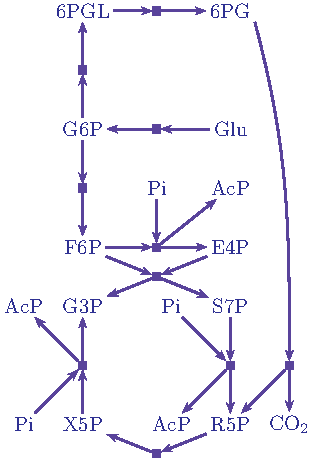
\includegraphics[width=\textwidth]{graphics/prolog/crn_metabolite.pdf}
        \caption{a reaction network showing the metabolism of carbohydrates~\cite{crn_metabolite}}
        \label{fig: crn1}
    \end{subfigure}%
    \hfill
    \begin{subfigure}{0.48\textwidth}
        \centering
        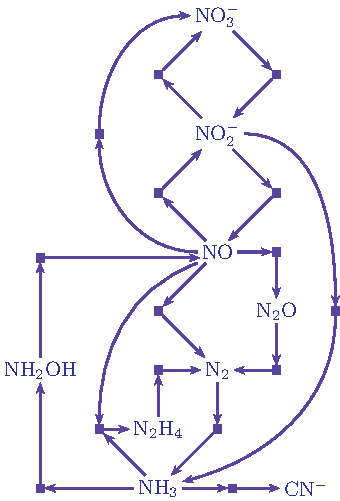
\includegraphics[width=\textwidth]{graphics/prolog/crn_atmosphere.pdf}
        \caption{a reaction network showing the reactions of atmospheric nitrogen~\cite{crn_atmosphere}}
        \label{fig: crn2}
    \end{subfigure}
    \vspace{0.5cm}
    \\
    \begin{subfigure}{\textwidth}
        \centering
        \vspace{0.5cm}
        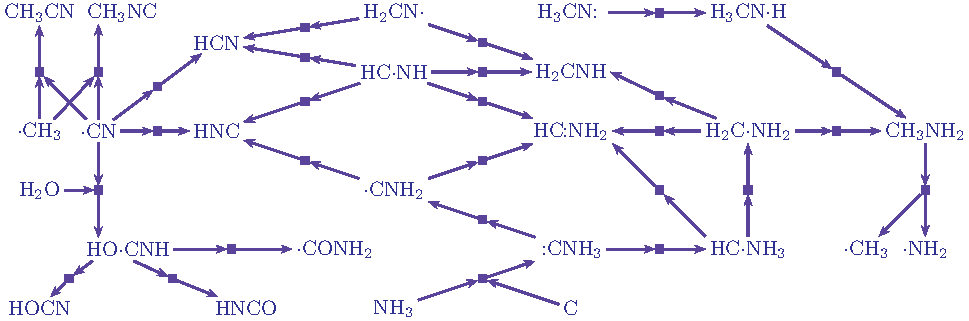
\includegraphics[width=\textwidth]{graphics/prolog/crn_astronomy.pdf}
        \caption{a reaction network showing reactions in the interstellar medium~\cite{crn_astronomy}}
        \label{fig: crn3}
    \end{subfigure}
    \vspace{0.2cm}
    \caption{Three chemical reaction networks from diverse contexts, attempting to show that reaction networks can be used to model diverse environments.}
    \label{fig: crns}
\end{figure}


The exploration of reaction networks to synthesize molecules has primarily been done experimentally in the wet laboratory. However, this process is labor intensive, costly, and limits the pace of exploration. \emph{In silico} modeling and exploration of reaction networks have the potential to speed up the process and guide manual efforts. The finer the physical details included in the modeling of the reaction networks, the more accurate the results can be expected to be. The ultimate way of doing that would be to construct the complex free energy landscape for the full reaction network, which then, in principle, would allow for the full simulation of reactions, as these are ultimately guided by the laws of thermodynamics.
However, this might be currently past any modeling and computational capacities available. 
Presently, algorithmic exploration of reaction networks by automated tools such as Reaction Mechanism Generator (RMG)~\cite{rmg2}, Chemotron~\cite{chemotron}, Yet Another Reaction Program (YARP)~\cite{yarp} and others, is limited to predicting a short sequence of reactions to a queried target molecule (often with no possible side-products). These tools have been applied to domains such as combustion chemistry~\cite{rmg2}, synthesis planning~\cite{retrosynthesis_comp,retrosynthesis_comp2,retrosynthesis_comp2}, reactions in metabolic systems~\cite{metabolic_comp,metabolic_comp2}, batteries, the atmosphere, the interstellar medium and so on. 
The diversity and varying approaches taken in characterizing reaction networks is evidence to the fact that generic methods are absent which work reasonable well across multiple and vastly differing application scenarios.

\section{Thermodynamics and Reaction Networks}

Equilibrium thermodynamics has been often used to determine the spontaneity of an isolated chemical reaction. Specifically, from the Gibbs free energy one can find the driving forces behind a reaction and determine whether its occurrence is favorable or not. Specifically in the context on reaction networks, chemical potentials can be used to determine if a given reaction is favorable in thermodynamical terms, and then only the favorable reactions are used in the exploration of the reaction networks.

However, before one can search for pathways in a reaction network, the network itself has to be constructed. This can be done in various ways. In one approach, the potential energy surface of a set of molecules is explored to elucidate trajectories with low-lying saddle points, separating the reactants from the products. Computationally intensive quantum mechanical calculations are used in most cases \cite{crn_expand_qm,crn_expand_qm3}, along with faster but less accurate semi-empirical methods in some \cite{yaks,empi1}.
Recently, generative diffusion models have also been used to perturb molecules to generate reaction networks with unknown mechanisms \cite{OA-ReactDiff,diffusion_ai}.
A different approach is to use reaction templates for iteratively expanding the network from a set of starting molecules, possibly in conjunction with filters to exclude specific reactions \cite{rmg2,molpher}.
Further approaches include the generation of the reaction network of interest in a one-shot heuristical process by an expert \cite{heuristic_expert}, or the loading of an existing network from a database \cite{reported_network}.

Once a reaction network is constructed, pathways can then be queried in the network using diverse strategies. Some general methods to search and analyze pathways in reaction networks can be found at \cite{search_crn} and ~\cite{search_crn2}. Previous work include Beam search based on suitable crafted scoring functions utilizing priority queues \cite{beam_search_pq}, as well as Monte-Carlo search trees extended with a method to sample efficient pathways \cite{mc_trees}.
Traditional path-finding algorithms such as A$^*$ algorithm~\cite{shortest_path_hypergraph2} and cutting-plan algorithm for an integer linear program~\cite{shortest_path_hypergraph1} have been used in previous work to find pathways between molecules.
Some analytical strategies have been used in the study of dynamics of pathways in reaction networks \cite{crn_dynamics,crn_dynamics2}, but they are often limited by the availability of kinetic data and the scale of the networks.

Moving on to studies specifically using thermodynamics to elucidate pathways in reaction networks, an example would be of~\cite{synthesis_planning_CRN_thermodynamics} which uses data provided by thermochemistry to suggest pathways in reaction networks through pathfinding algorithms and a linear combination of the lowest cost pathways in that network. 
In thermodynamics-based metabolic flux analysis~\cite{hatz_thermo_flow}, the mass balance constraints of metabolic flux analysis are augmented by additional thermodynamic constraints to produce flux distributions and metabolite activity profiles free from thermodynamic infeasibilities.
In \cite{seifert_thermodynamics_CRN_JCP}, nonequilibrium thermodynamics was developed to explore reaction networks, employing a stochastic trajectory-based approach to define energy, entropy, and heat dissipation along reactions.
Building upon stochastic thermodynamics, a nonequilibrium thermodynamic framework for open reaction networks has been formulated~\cite{esposito_thermodynamics_CRN_PRX}, governed by deterministic rate equations with mass action kinetics and introducing a nonequilibrium Gibbs free energy quantifying the minimal work required to induce nonequilibrium states from an equilibrium state.
This nonequilibrium Gibbs free energy is minimized as the open detailed-balanced network relaxes to an equilibrium state, aligning with the maximum entropy principle.
Circuit theory has been applied to reaction networks~\cite{esposito_circuit_theory_CRN_PRX} extending the chemical analogs of Kirchhoff’s laws to predict reaction currents within complex reaction networks.
\cite{ILP_paper2} utilizes linear programming to identify complex balanced realizations of mass action kinetics in reaction networks.
\cite{ILP_paper2, ILP_paper3, ILP_paper4} have introduced numerical procedures for determining weakly reversible reaction networks using integer linear programming (ILP), emphasizing the importance of ILPs in identifying specific network properties.
Mixed integer linear programming has been employed to prune reaction networks using experimental data and to understand complex chemical systems in~\cite{ilp_CRN_infer}.

Much of the work cited in the preceding paragraph primarily focuses on theoretical formulations, with few executable implementations.
In contrast, MØD~\cite{mod_web,jakob_software} is a software package developed to generate and analyze reaction networks.
M{\O}D models molecules using undirected graphs with attributes, hence with each atom explicitly represented, and reactions are modeled by rules for transforming molecule graphs.
Reaction networks can automatically be generated from a set of rules and a set of starting molecules using the graph transformation engine of M{\O}D.
The outcome is a directed multihypergraph representing the reaction network.
The pathways in such reaction networks can then be queried using integer hyperflows as a formal model~\cite{jakob_integer_hyperflows}
and the reaction network can be queried using computational means for the presence of the specified pathway.
This framework allows for a flexible, yet precise specification of pathways and a search for such pathways by computational means.
However, the methodology~\cite{jakob_integer_hyperflows} currently does not incorporate any dynamics in the modeling of the reaction network.

A critical assumption while using thermodynamics to search for pathways in reaction networks is that the reactions in the network are in equilibrium, and the concentration of the molecules are steady. Given enough time, a reaction network will reach a steady-state where the favourable pathways are determined by the overall free energy landscape, and corresponds to a configuration which has the minimum free energy of the molecules. However, these assumptions might (over)simplify practicalities that might hinder thermodynamically favorable reactions from occurring.

\section{Energy Barriers and Reaction Networks}

Kinetic studies of individual reactions have provided valuable insight into their mechanisms which are often not provided by thermodynamics alone, which in turn can generate ways to optimize the reaction to suit the overall synthesis goals.
Despite the `dynamics' in the name, thermodynamics does not help to elucidate the `dynamics' of the system: how fast does the pathway in question run and how quickly does the system equilibrate? For example, under atmospheric conditions, the conversion of diamond to graphite is thermodynamically favorable. However, the energy barrier for this conversion is high, so, thankfully, for all practical purposes `diamonds are forever'. 
Therefore, kinetic parameters of reactions, such as the free energy barrier or the rate constant, might provide better alternatives for characterizing pathways. Theoretical and computational modeling attempts to offer a possibility for analyzing the kinetics in reaction networks to various degrees of accuracy and computational efficiency, depending on the level of abstraction employed.

Except for approaches where the reaction network is generated by the exploration of the potential energy surface, individual reactions will need to be annotated with the kinetic parameters from a separate source, such as databases \cite{database_energy_barriers}, estimations informed by experiments \cite{reported_network}, or dedicated quantum mechanical calculations \cite{CRN_qm}.
Empirical relations, deduced via machine learning on available data on kinetics of reactions, have been used to estimate kinetic parameters for reactions \cite{ml_energy_barrier,ml_energy_barrier2,ml_energy_barrier3,ml_energy_barrier4,ml_energy_barrier5,ml_energy_barrier6,ml_reaction_barrier7}. However, these methods have limited success on `out of class' molecules \cite{scaling_limitations}. 

Although more expensive, strategies that base the search for pathways in reaction networks based on the kinetics ultimately increase the utility of the search process of pathways to the queried target molecule, with the trade-off of increased computational costs. This is because additional calculations are required to estimate the energy barriers of the reactions (than just computing the chemical potentials of the molecules in the reaction network) but it increases the realism in the resulting search. This results in an approach more faithful in modeling the physical system and which might be of more utility for potential users.

An ideal pathway enumeration algorithm would only explore a subset of reactions in the possible molecular space that are only necessary for the more realistic pathways. One way of quantifying how `realistic' a pathway is (or in other words, how probable it is for the pathway to be observed in a real reactor system) would be to score it using some metric, based on physical parameters. However, it is not generally easy to annotate each reaction with this metric and determine which reaction channels are more favoured in practice. This leads to characterization of more reactions than the minimum required. Many methods use the exploration strategy of characterizing all immediate reaction channels and prioritizing only the ones that are immediately important, for further elucidation of the pathway. This variant of a greedy algorithm considers only the most favoured channel at each steps and ignores the rest completely. A more inclusive and forward-looking algorithm would investigate multiple reaction channels at each step to determine most of the pathways with large contributions to the flow of matter in an attempt to identify the most optimal pathways. However, in reality, unlike in enumerated fixed pathways, the constituent intermediate molecules are not constrained to react only through the reaction specified by the pathway. They reaction through various side reactions resulting in reduction of performance of the pathway than the optimal calculated.

\section{Contribution of this work}

In this work, thermodynamic principles are incorporated into the existing hyperflow model in M{\O}D in Chapter~\ref{ch:thermodynamic_model}.
In particular, we develop methods based on mixed integer linear programming (MILP) that allow thermodynamic constraints to be added to the specification of pathways extending the available search for the pathways in the M{\O}D framework.
Our methods can return several alternative pathways, and these can be ranked on the basis of thermodynamic-based metrics. 
It would be helpful to the reader to point out that in this work, reaction networks are modeled on a level of abstraction where the network is represented by a hypergraph and individual reactions are represented by directed hyperedges \cite{jakob_integer_hyperflows}.
This enables us to capture the many-to-many mapping in chemical reactions which is not possible easily usinging simple directed graphs (with edges directed from one vertex to another vertex).
The nodes of the hypergraph are molecular graphs (with their nodes representing atoms and edges representing bonds) and hence the modeling is atomistically explicit.

We note that returning multiple pathways can significantly increase the practical value of the investigations.
Models of reaction networks and estimations of thermodynamic parameters are inherent simplifications of reality.
Hence, any single pathway returned may turn out to be less desirable in the face of further details of the chemical situation.
Hence, having a number of highly ranked pathways available from which the practitioner can choose is a more robust strategy.

The assignment of chemical potentials to the molecules in the reaction network to calculate the Gibbs free energies for its reactions is done using the semi-empirical method GFN2-xTB~\cite{grimme_xtb} in the current implementation, which provides a good balance between accuracy of the thermodynamic parameters and the ability to handle larger molecules.
However, it can be replaced by any other method to assign chemical potentials if the user desires so.
For generality we refer to the chosen method as a thermodynamic oracle.
We note that using a thermodynamic oracle to calculate the chemical potentials of the molecules in an automated fashion has the added benefit of being applicable in rule-based generative systems where the chemical space is expanded on the fly and the molecules generated are unknown at the start.

To the best of our knowledge, there currently does not exist a computational method for searching for pathways in reaction networks based on thermodynamic constraints that combines MILP with the wide applicability and speed of semiempirical tight-binding methods.

In Chapter~\ref{ch:refined_model}, we further extend the framework developed to incorporate an objective measure to rank pathways in a reaction network maximizing the probability of the entire pathway based on physical principles. 
Based on the notion that energy barriers of reactions are the determining factor for the kinetics of the network, we develop an automated methodology for computing such energy barriers, building on a combination of an array of existing computational tools. A key novelty is that in contrast to the standard manual intervention required to generate reaction trajectories from which the reaction barrier can be estimated, we try to automate this part of the process.
Lastly, we formulate an integer linear program which allows the user to specify queries for pathways in the network in a very flexible and generic way. Solving this integer linear program returns all pathways fulfilling the criteria, ranked by the objective measure mentioned above.
In short, this gives an automated, general, and flexible methodology for analyzing reaction networks, a methodology which offers a speed-up over manual search for pathways but with comparable quality.

To exemplify its utility in Chapter~\ref{ch:casestudy2}, we apply it to a reaction network expanded from the molecules 2-hydroxyethanenitrile, ammonia and water, where we query for pathways to glycine, an amino acid, and 2-hydroxyethanoic acid, a molecule encountered in photorespiration in plants.

\section{Contributing Papers and Overview}

Most of the text and illustrations in this document is taken from the following papers:

\begin{enumerate}
	\item \textsf{\textsl{Pal, Adittya, Rolf Fagerberg, Jakob Lykke Andersen, Christoph Flamm, Peter Dittrich, and Daniel Merkle. "Finding thermodynamically favorable pathways in chemical reaction networks using flows in hypergraphs and mixed-integer linear programming." Journal of Chemical Information and Modeling 65, no. 13 (2025): 6772-6787}}
	
	Chapters 2, 4 and 5 are taken from this peer-reviewed paper, while parts of Chapters 1 and 8 are based on the text from it. 
	
	\item \textsf{\textsl{Pal, Adittya, Rolf Fagerberg, Jakob Lykke Andersen, Peter Dittrich, and Daniel Merkle. "Finding Pathways in Reaction Networks Guided by Energy Barriers Using Integer Linear Programing." Molecular Informatics 45, no. 3 (2026): e70021}}
	
	Chapters 3, 6 and 7 are taken from this peer-reviewed paper, while parts of Chapters 1 and 8 are based on the text from it. 
\end{enumerate}

The rest of this thesis is organized as follows:
In Chapter~\ref{ch:toolbox}, we give the definitions underlying our modeling of reaction networks and pathways.
In Chapter~\ref{ch:preliminaries}, we give an overview of the network construction process by the recursive application of graph transformation rules to an input set of molecular graphs.
In Chapter~\ref{ch:thermodynamic_model}, which constitutes the core part of the work extending the integer hyperflows with thermodynamic constraints and an objective function, we give the details of the proposed framework and comparison with some existing frameworks.
In Chapter~\ref{ch:casestudy1}, we demonstrate the usability of the method proposed in Chapter~\ref{ch:thermodynamic_model} by applying them on a reaction network constructed from hydrogen cyanide, ammonia and water.
In Chapter~\ref{ch:refined_model}, we refine the framework proposed in Chapter~\ref{ch:thermodynamic_model} with energy barriers, an alternative objective function, enumeration of pathways and partial ordering of the molecules in the returned pathways.
In Chapter~\ref{ch:casestudy2}, we demonstrate the usability of the method proposed in Chapter~\ref{ch:refined_model} by applying them on a reaction network constructed from glycolonitrile, ammonia and water.
In Chapter~\ref{ch:conclusion}, we offer a conclusion to the work presented here.
Some additional work have been placed in appendices.


%************************************************
\chapter{Definitions}
\label{ch:toolbox}
%************************************************

{\sffamily\slshape The text in this chapter is identical to Section 2 of the published version of the preprint at \href{https://arxiv.org/abs/2411.15900}{arXiv:2411.15900} along with the figures.\\}

In this chapter, the mathematical models for chemical reaction networks and pathways in them are presented,
namely directed hypergraphs and integer hyperflows, respectively.
This section is based on previous work which have used these concepts \cite{jakob_reactions_hypergraph,jakob_integer_hyperflows}. 

%%%%%%%%%%%%%%%%%%%%%%%%%%%%%%%%%%%%%%%%%%%%%%%%%%%%%%%%%%%%%%%%%%%%%%%%%%
\section{Directed Hypergraphs}
\label{sec:hypergraphs}
%%%%%%%%%%%%%%%%%%%%%%%%%%%%%%%%%%%%%%%%%%%%%%%%%%%%%%%%%%%%%%%%%%%%%%%%%%

A chemical reaction network consists of set of molecules $V$ and a set of reactions $E$.
Each reaction $e\in E$ is generally a many-to-many mapping of molecules,
which can be written~\cite{christoph_reaction_network_chemical} as the formal sum
\begin{equation*}
        e \colon \sum_{v\in V} s_{ve}^{-} v \longrightarrow \sum_{v\in V} s_{ve}^{+} v 
        \label{chemical_equation}
\end{equation*}
where $s_{ve}^{-}$ and $s_{ve}^{+}$ denote the stoichiometric coefficients,\\
\begin{tabular}{ll}
$s_{ve}^{-}$ & is the number of molecules of $v$ that are used \\
$s_{ve}^{+}$ & is the number of molecules of $v$ that are produced \\
\end{tabular}

\noindent by reaction~$e$.
\footnote{Note that the use of $^+$ and $^-$ is swapped compared to the notation in the referred previous work using hyperflows~\cite{jakob_integer_hyperflows}).}
The sum is over the entire set of molecules $V$ in the chemical reaction network,
and for molecules $v$ that do not take part in a particular reaction $e$, we have $s^-_{ve} = s^+_{ve} = 0$

A chemical reaction network is formally well represented~\cite{jakob_integer_hyperflows} as a directed multi-hypergraph~$(V, E)$, where

\begin{tabular}{l}
the set~$V$ of vertices models molecules and \\
the set~$E$ of directed multi-hyperedges models reactions. \\
\end{tabular}

A directed multi-hyperedge $e\in E$ is an ordered pair $(e^-, e^+)$ of multisets of vertices, which represents a reaction in the chemical reaction network.
The elements of $e^-$ model the reactants of the reaction, with each reactant $v$ appearing $s^-_{ve}$ times,
and correspondingly $e^+$ and $s^+_{ve}$ model the products of the reaction. An example hyperedge representing a chemical reaction is shown in Figure~\ref{fig: hyperedge}.
\newpage

\begin{figure}[!t]
	\centering
	\vspace{0.5cm}
    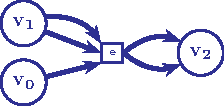
\includegraphics[scale=1.5]{graphics/chapter0/hyperedge.pdf}
    \vspace{0.5cm}
    \caption{A directed hyperedge, which represents a reaction where one copy of the molecule represented by the vertex $v_0$ reacts with two copies of $v_1$ to produce two copies of $v_2$. 
    This hyperedge can be considered to represent the reaction with the vertices representing the molecules: $v_0 \equiv$ O$_2$, $v_1 \equiv$ H$_2$ and $v_2 \equiv$ H$_2$O and the directed hyperedge representing the chemical reaction $e :$ O$_2$ + 2 H$_2$ $\longrightarrow$ 2 H$_2$O.}
    \label{fig: hyperedge}
\end{figure}

\begin{figure}[!ht]
    \centering
    \vspace{1cm}
    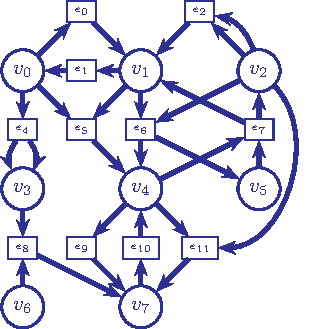
\includegraphics[scale=1.5]{graphics/chapter0/hypergraph.pdf}
    \vspace{0.4cm}
    \caption{A directed hypergraph, where circles are vertices and the squares are hyperedges.
    Hyperedges with multiple copies of a vertex as source or target are depicted with parallel arrows.
    See for instance~$e_4$, which has $v_3$ twice as a target and thus represents the reaction $e_4 : v_0 \rightarrow 2 v_3$. Hyperedges allow the many-to-many relations in chemical reaction to be captured in themodelling unlike edges in simple directed graphs.}
    \label{fig: hypergraph}
\end{figure}

\newpage

Figure~\ref{fig: hypergraph} depicts a hypergraph with eight vertices and eleven hyperedges.
As examples, \\
\begin{tabular}{ll}
	hyperedge~$e_0$ &$\equiv (\{v_0\}, \{v_1\})$ \\
	& represents the one-to-one reaction $v_0\rightarrow v_1$, \\
	hyperedge~$e_3$ &$\equiv (\{v_0, v_1\}, \{v_3\})$  \\
	& represents the many-to-one reaction \\
	& $v_0 + v_1\rightarrow v_3$, \\
	hyperedge~$e_2$ &$\equiv (\{v_2, v_2\}, \{v_1\})$ \\
	& represents the many-to-one reaction $2 v_2\rightarrow v_1$, \\
	hyperedge~$e_4$ &$\equiv (\{v_3\}, \{v_0, v_1\})$ \\
	& represent the one-to-many reaction \\
	& $v_3\rightarrow v_0 + v_1$, \\
	hyperedge~$e_7$ &$\equiv (\{v_3\}, \{v_5, v_5\})$ \\
	& represent the one-to-many reaction \\
	& $v_3\rightarrow 2 v_5$, and \\
	hyperedge~$e_9$ & $\equiv (\{v_3, v_4\}, \{v_7, v_8\})$ \\
	& represents the many-to-many reaction \\
	& $v_3 + v_4\rightarrow v_7 + v_8$.\\
\end{tabular}

On a related note, standard usage of the term `reaction' implies the breaking and forming of chemical bonds.
However, physical processes that do not alter the set of bonds in a molecule yet involve energy transformations, thereby affecting the molecule's ability to participate in a reaction.
For instance, some reactions occur only when a molecule is excited into a higher energy state, or certain molecules (such as phosphorus or sulfur) are in specific phases.
Although such transitions are not conventionally termed `reactions,' they are elementary processes accompanied by a change in free energy.
Consequently, in the rest of this paper we will use the term `reaction' to denote this broader set of relations between classes of molecules. 

%%%%%%%%%%%%%%%%%%%%%%%%%%%%%%%%%%%%%%%%%%%%%%%%%%%%%%%%%%%%%%%%%%%%%%%%%%
\section{Integer Hyperflows}
\label{sec:hyperflows}
%%%%%%%%%%%%%%%%%%%%%%%%%%%%%%%%%%%%%%%%%%%%%%%%%%%%%%%%%%%%%%%%%%%%%%%%%%
A pathway is a set of reactions that transforms some available source molecules into desired target molecules.
To model pathways formally, the concept of an \emph{integer hyperflow}~$f$ in a hypergraph~$\mathcal{H} = (V,E)$ was introduced by~\cite{jakob_integer_hyperflows}.

A pathway is viewed as a vector $f_E \in \mathbb{N}_{0}^{|E|}$,
i.e., an assignment of a non-negative integer to each edge in~$E$, denoting how many times the corresponding reaction appears in the pathway.
Additionally, two vectors $f_{\text{in}} \in \mathbb{N}_{0}^{|V|}$ and $f_{\text{out}} \in \mathbb{N}_{0}^{|V|}$ denote for each molecule in~$V$ the amount of it consumed as source molecule, respectively produced as target molecule, by the pathway.

\begin{figure}[!t]
    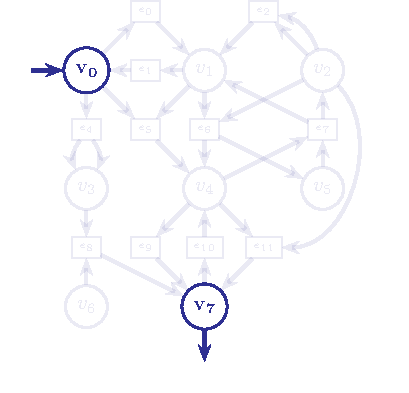
\includegraphics[scale=1.5]{graphics/chapter0/flowQuery.pdf}
    \vspace{0.5cm}
    \caption{An integer hyperflow query in the directed hypergraph from Figure~{ref: hypergraph}, where $v_0$ is specified as the source and $v_7$ is specified as the target. 
    The exact inflow and outflow on these vertices are not specified, and the hyperpaths in Figure~\ref{fig: hyperpath1}, \ref{fig: hyperpath2}, \ref{fig: hyperpath3}, \ref{fig: hyperpath4} and \ref{fig: hyperpath5} would be valid solutions of this flow query if the required additional sets of vertices is allowed as sources (which are {\O}, $\{v_2\}$, $\{v_1\}$, $\{v_2\}$, $\{v_6\}$ respectively).
    If additional vertices are not allowed as sources, only the hyperpath in Figure~\ref{fig: hyperpath1} is a valid solution.}
    \label{fig: flow_query}
\end{figure}


The pathway's net effect on the number of molecules in the system is specified entirely by $f_{\text{in}}$ and $f_{\text{out}}$.
\begin{equation}
    \mathbf{S}^+\cdot f_E  - \mathbf{S}^-\cdot f_E =  f_{\text{out}} - f_{\text{in}}
    \label{int_hyperflow_matrix}
\end{equation}
where

\begin{tabular}{ll}
$\mathbf{S}^-$ & is a $|V|\times |E|$ matrix with entries~$s_{ve}^-$ \\
$\mathbf{S}^+$ & ia a $|V|\times |E|$ matrix with entries~$s_{ve}^+$ \\
\end{tabular}

\noindent (recall from definition of hypergraphs that $s_{ve}^-$ and $s_{ve}^+$ are the numbers of molecule $v$ consumed and produced by reaction $e$).
In hypergraph terminology, $\mathbf{S}^-$ and $\mathbf{S}^+$ are the out-incidence matrix and the in-incidence matrix, respectively.% dont remove this comment, it escapes the newline
\footnote{
    In other settings, $\mathbf{S}^-$ and $\mathbf{S}^+$ are called the reactant stoichiometric matrix and the product stoichiometric matrix.
    One can also meet a single stoichiometric matrix, defined as $\mathbf{S} = \mathbf{S}^+ - \mathbf{S}^-$.
    This latter version is less expressive for chemical reaction network modeling, as the role of catalysts and autocatalytic molecules cannot be captured.
    In some contexts, $f_{\text{in}}$ and $f_{\text{out}}$ are called the external compounds.
}
The matrices $\mathbf{S}^-$ and $\mathbf{S}^+$ for the hypergraph in Figure \ref{fig: hypergraph} are shown in Figure \ref{fig: stoichoimetric_matrix}.

\begin{figure}[!t]
	\centering
	\begin{subfigure}{0.75\textwidth}
		\begin{small}
		\[       
		    \kbordermatrix{
		            &e_0&e_1&e_2&e_3&e_4&e_5&e_6&e_7&e_8&e_9&e_{10}\\
		        v_0 & 1 &   &   & 1 &   &   &   &   &   &   &   \\
		        v_1 &   & 1 &   &   &   & 1 &   &   &   &   &   \\
		        v_2 &   &   & 2 &   &   & 1 &   &   &   &   & 1 \\
		        v_3 &   &   &   &   & 1 &   &   & 1 &   &   &   \\
		        v_4 &   &   &   &   &   &   & 1 &   &   & 1 & 1 \\
		        v_5 &   &   &   &   &   &   &   &   &   &   &   \\
		        v_6 &   &   &   &   &   &   &   &   &   &   &   \\
		        v_7 &   &   &   &   &   &   &   &   &   &   &   \\
		        v_8 &   &   &   &   &   &   &   &   &   &   &  
		    }
		\]
		\end{small}
		\caption{in-incidence matrix}
		\label{in_incidence}
    \end{subfigure}
    \\
    \vspace{0.5cm}
    \begin{subfigure}{0.75\textwidth}
    	\begin{small}
		\[
		    \kbordermatrix{
		            &e_0&e_1&e_2&e_3&e_4&e_5&e_6&e_7&e_8&e_9&e_{10}\\
		        v_0 &   & 1 &   &   & 1 &   &   &   &   &   &   \\
		        v_1 & 1 &   & 1 &   &   &   & 1 &   &   &   &   \\
		        v_2 &   &   &   &   &   &   & 1 &   &   &   &   \\
		        v_3 &   &   &   & 1 &   &   &   &   &   &   &   \\
		        v_4 &   &   &   &   &   & 1 &   &   &   &   &   \\
		        v_5 &   &   &   &   &   &   &   & 2 &   &   &   \\
		        v_6 &   &   &   &   &   &   &   &   & 1 &   & 1 \\
		        v_7 &   &   &   &   &   &   &   &   &   & 1 &   \\
		        v_8 &   &   &   &   &   &   &   &   &   & 1 & 
		    }
		\]
		\end{small}		
		\caption{in\\out-incidence matrix}
		\label{out_incidence}
	\end{subfigure}
    \caption{A representation of the hypergraph from Figure \ref{fig: hypergraph} as \ref{out_incidence} an out-incidence matrix $\mathbf{S}^-$ and \ref{in_incidence} an in-incidence matrix $\mathbf{S}^+$.
    Only non-zero entries are shown.
    Since the hypergraph has $9$ vertices and $11$ hyperedges, the matrices have dimensions $9 \times 11$.}
    \label{fig: stoichoimetric_matrix}
\end{figure}

To unify the three vectors~$f_E$, $f_{\text{in}}$, and $f_{\text{out}}$ into a single flow vector on hyperedges,
\cite{jakob_integer_hyperflows} introduced for each $v \in V$ two so-called half-edges

\begin{tabular}{l}
$e_v^+ = (\emptyset, v)$ and \\
$e_v^- = (v, \emptyset)$ \\
\end{tabular}

\noindent These represent the production of~$v$ as source molecule addition to the system and the consumption of~$v$ as target molecule removal from the system, respectively.
Setting
$$
\begin{array}{lcl}
E^+ & = & \{ e_v^+ \mid  v \in V\}\\
E^- & = & \{ e_v^- \mid  v \in V\}\\
\overline{E} & = & E \cup E^+ \cup E^-,\\
\end{array}
$$
\cite{jakob_integer_hyperflows} introduced the extended hypergraph $\overline{\mathcal{H}} = (V, \overline{E})$
and defined an \emph{integer hyperflow} to be a vector $f \in \mathbb{N}_{0}^{|\overline{E}|}$ satisfying the flow conservation constraint
\footnote{A detailed discussion of how integer hyperflows relate to, and differ from, other similar concepts such as elementary modes, extreme pathways, and flux balance analysis can be found in Section 2.6 of~\cite{jakob_integer_hyperflows}.}
\begin{equation}
    \forall v\in V\colon \sum_{ e\in \overline{E} } s_{ve}^+ f_e - \sum_{ e\in \overline{E} } s_{ve}^- f_e = 0 
    \label{int_hyperflow_jakob}
\end{equation}
where,

\begin{tabular}{ll}
$s_{ve}^-$ & an entry in the $|V|\times |\overline{E}|$ out-incidence matrix of $\overline{\mathcal{H}}$ \\
$s_{ve}^+$ & an entry in the $|V|\times |\overline{E}|$ in-incidence matrix of $\overline{\mathcal{H}}$ \\
$f_e$ & an entry in $f$ \\
\end{tabular}

\newpage
\begin{figure}[!ht]
    \centering
    \begin{subfigure}{0.48\textwidth}
        \centering
        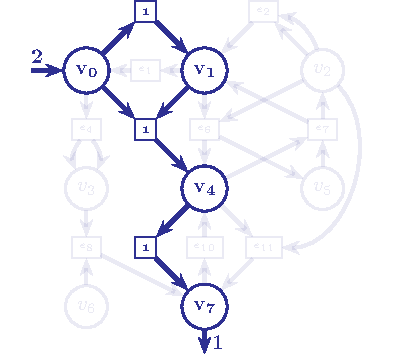
\includegraphics[width=\textwidth]{graphics/chapter0/hyperpath1.pdf}
        \caption{hyperpath 1}
        \label{fig: hyperpath1}
    \end{subfigure}%
    \hfill
    \begin{subfigure}{0.48\textwidth}
        \centering
        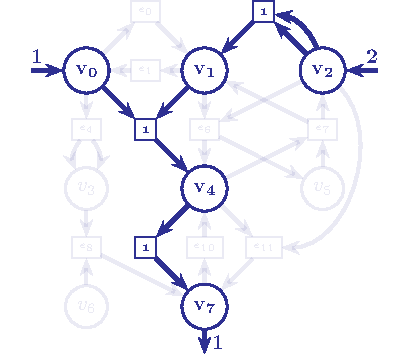
\includegraphics[width=\textwidth]{graphics/chapter0/hyperpath2.pdf}
        \caption{hyperpath 2}
        \label{fig: hyperpath2}
    \end{subfigure}
    \\
    \vspace{0.5cm}
    \begin{subfigure}{0.48\textwidth}
        \centering
        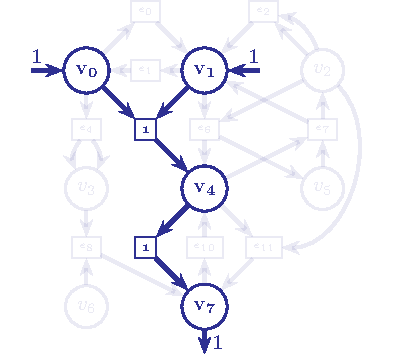
\includegraphics[width=\textwidth]{graphics/chapter0/hyperpath3.pdf}
        \caption{hyperpath 3}
        \label{fig: hyperpath3}
    \end{subfigure}%
    \hfill
    \begin{subfigure}{0.48\textwidth}
        \centering
        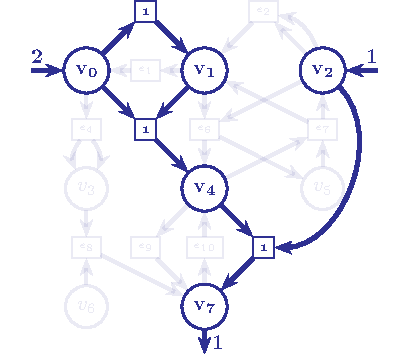
\includegraphics[width=\textwidth]{graphics/chapter0/hyperpath4.pdf}
        \caption{hyperpath 4}
        \label{fig: hyperpath4}
    \end{subfigure}
    \\
    \vspace{0.5cm}
    \begin{subfigure}{0.48\textwidth}
        \centering
        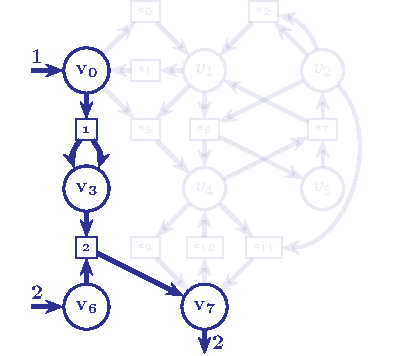
\includegraphics[width=\textwidth]{graphics/chapter0/hyperpath5.pdf}
        \caption{hyperpath 5}
        \label{fig: hyperpath5}
    \end{subfigure}%
    \hfill
    \begin{subfigure}{0.48\textwidth}
        \centering
        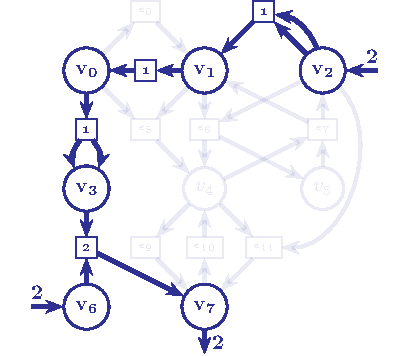
\includegraphics[width=\textwidth]{graphics/chapter0/hyperpath6.pdf}
        \caption{hyperpath 6}
        \label{fig: hyperpath6}
    \end{subfigure}
    \vspace{0.4cm}
    \caption{Six possible integer hyperflows \ref{fig: hyperpath1}, \ref{fig: hyperpath2}, \ref{fig: hyperpath3}, \ref{fig: hyperpath4}, \ref{fig: hyperpath5}, and \ref{fig: hyperpath6} in the hypergraph from Figure \ref{fig: hypergraph}, each representing a pathway,
    where hyperedges with non-zero flow are drawn in bold. The integers in the boxes represent the hyperflow assigned to the respective hyperedge in the pathway.}
    \label{fig: hyperflow}
\end{figure}

\newpage
\noindent The constraint in Equation~\eqref{int_hyperflow_jakob} is easily seen to be equivalent to the constraint in Equation~\eqref{int_hyperflow_matrix}. 

In Figure~\ref{fig: hyperflow}, six possible hyperflows in a hypergraph are depicted.
Unboxed integers are flow values on half-edges, while boxed integers are the flow values for hyperedges in $E$.
The inflow and the outflow are depicted as half-edges in and out of the source and target vertices of the pathway.
For clarity, only half-edges with non-zero flow values are shown.

One key feature of integer hyperflows is that they give a flexible and generic way to \emph{specify} pathways via constraints on the flow on half-edges.
This may be as straight-forward as specifying an overall reaction for the pathway by fixing the flow on the half-edges for the molecules in the source and target sets and setting the flow to zero for the rest of the half-edges.
Or one may specify upper and lower limits for some half-edges and free values for others,
for instance to ask if there is any way to produce at least some target molecules using any amount of source molecules,
while at the same time allowing waste products.

Then a \emph{search} for pathways fulfilling the specification amounts to finding flow vectors~$f$ obeying those constraints, in addition to the constraint in Equation~\eqref{int_hyperflow_jakob}.
Since integer hyperflows are integer valued, it is natural to model the situation via the ILP formalism and search for~$f$ using an ILP solver.
This idea has been implemented as part of the software system~MØD~\cite{mod_web}.
The result is a powerful and flexible tool for specifying and searching for pathways (integer hyperflows) in a given chemical reaction network (hypergraph).
The flexibility is further increased by the possibility of having flow values in the ILP objective function, such that e.g.\ flow solutions allowing but minimizing waste can be found.
Also the flow values on non-half-edges can enter the specification and/or optimization,
allowing e.g.\ the search for solutions minimizing the use of a given reaction deemed particularly expensive to include in the pathway.

\section{Hyperflows and Fluxes}
\label{sec: comparison}

In this section, we give a comparison of our workflow with existing methods. Constraint-based models such as flux balance analysis also use constraint programming with an objective function that is optimized. For instance, open-source tools such as COBRApy~\cite{cobrapy} perform flux analysis on a reaction network supplied to them. However, such tools do not construct the network on the fly in a generative way--- rather the reaction network has to be constructed beforehand using some other tool. Flux balance analysis generates a flux vector for the reactions in the network which is allowed to contain floating-point values, while our method accepts only integers as a valid hyperflow for a reaction, which is more aligned with the standard notion of a pathway. Formulating a flux balance analysis on the network would be equivalent to an LP relaxation of the pathway query problem using integer hyperflows for the same network. A linear program (LP) can be solved in polynomial time while an ILP is NP-hard. However, formulating the search for pathways to a queried molecule in a reaction network offers some advantages.

\begin{figure}
    \centering
    \begin{subfigure}{\textwidth}
        \centering
        \includegraphics[scale=1.0]{graphics/chapter0/example_network.pdf}
        \vspace{0.4cm}
        \caption{An example reaction network with $4$ molecules and $3$ reactions.}
        \label{fig:example_network}
    \end{subfigure}\\
    \vspace{0.8cm}
    \begin{subfigure}{\textwidth}
        \centering
        \includegraphics[scale=1.0]{graphics/chapter0/example_flux.pdf}
        \vspace{0.4cm}
        \caption{A flux distribution in the network which produces an outflow of $1.5$ for $v_3$.}
        \label{fig:example_flux}
    \end{subfigure}\\
    \vspace{0.8cm}
    \begin{subfigure}{\textwidth}
        \centering
        \includegraphics[scale=1.0]{graphics/chapter0/example_flow.pdf}
        \vspace{0.4cm}
        \caption{An assignment of integer hyperflows in the network which produces an outflow of $1$ for $v_3$.}
        \label{fig:example_flow}
    \end{subfigure}
    \vspace{1cm}
    \caption{Comparison of flux balance analysis and an integer hyperflow in an example reaction network.}
    \label{fig:comparison}
\end{figure}

There exists reaction networks where the optimal solutions from the ILP formulated by our modeling and the relaxed LP from flux balance analysis differ. Consider the reaction network shown in Figure~\ref{fig:example_network} with the following formulation of the problem:
\begin{align*}
    &\max \left( \text{outflow}(v_3) \right) \\
    \text{subject to: } &\text{inflow}(v_0) + \text{inflow}(v_1) +\text{inflow}(v_2) \leq 3
\end{align*}
The optimal flux distribution yields an objective value of $1.5$ with the assigned fluxes shown in Figure~\ref{fig:example_flux} while our method assigns the integer hyperflows shown in Figure~\ref{fig:example_flow} in one of the three optimal solutions with objective value $1$. The other two solutions assign the hyperflows $(0,1,1)$ and $(1,1,0)$ to the hyperedge set $(e_1,e_2,e_3)$ respectively.

The ILP solution space is a subset of the LP feasible reaction and therefore, the objective value for the optimal solution for the relaxed LP will always be as at least as large as the objective value of optimal solution for the corresponding ILP. This is illustrated in the example shown in Figure~\ref{fig:comparison} too. As the result, the fluxes and the structure of the solution is often different from those if they were constrained to be integers.

Restricting hyperflows to integers makes physical sense because molecules occur and react in discrete quantities.
Actually, small molecular counts in several biological settings (often involving trace amounts of enzymes and inhibitors affecting multiple iterations of the same pathway) and physical cases (as in chain reactions and cascades) do not allow arbitrary scaling of the number of molecules, as the use of real-valued fluxes by flux balance analysis assume.
When a small number of molecules are encountered in a scenario as above (or in scenarios with appearances of a rare but significant molecule in the system), the discrete nature of the molecules becomes more pronounced.

Another feature of our proposed method is the enumeration of alternative pathways with disjoint set of hyperedges ranked on the basis of a chosen objective function. While flux balance analysis offers the possibility to find alternative pathways~\cite{fba_alternative_pathways}, they have the same objective value but a different flux distribution in the network. This differs from the enumeration of solutions in the current method which offers a list of pathways ordered by the increasing value of the objective function for the user to choose from. Enumerating solutions over variables with a continuous domain is difficult using indicator variables and biimplications as in constraints \ref{biimp1}  and \ref{biimp2}. The enumeration of solutions offers diverse pathways to the queried molecules and makes the method more robust to uncertainties in the weights assigned to the hyperedges.

\begin{refsection}
%************************************************
\chapter{Preliminaries}
\label{ch:preliminaries}
%************************************************

{\sffamily\slshape This chapter is identical to Appendix A and B of the published version of the preprint at \href{https://arxiv.org/abs/2504.10609}{arXiv:2504.10609}.\\}

While one might choose to represent a reaction formally by \eqref{chemical_equation}, for more practical scenarios, it is just a collection of reactant molecules (with their multiplicities) that gets converted into a collection of product molecules (with some different multiplicities). For example,\\

\begin{center}
\begin{tiny}
\begin{tabular}{ccccccc}
     \textcolor{Blue}{$e_1$} &\textcolor{Blue}{:} &\textcolor{Blue}{\chemfig{HO-[:30]-[:-30]~[:-30]N}} &\textcolor{Blue}{+} &\textcolor{Blue}{\chemfig{H_2O}} &\textcolor{Blue}{$\longrightarrow$} &\textcolor{Blue}{\chemfig{HO-[:-30]-[:30](-[:90]OH)=[:-30]NH}} \\
     && \textcolor{Blue}{$v_0$} && \textcolor{Blue}{$v_2$} && \textcolor{Blue}{$v_3$}
\end{tabular}
\vspace{0.5cm}
\end{tiny}
\end{center}

This reaction is a two-to-one map which converts molecules $\{v_0, v_1\}$ to $\{v_3\}$. In a hypergraph, we choose to represent this map graphically as
\begin{center}
    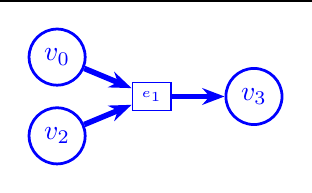
\begin{tikzpicture}[scale=1.0, color=Blue]    
        \tikzset{
        	vertex/.style = {shape=circle, line width=1pt, draw = Blue, text = Blue, align = center},
        	vertex2/.style = {shape=rectangle, line width=0.5pt, draw = Blue, text = Blue, align = center},    
            edge/.style = {->, color=Blue, line width = 2pt, -{Stealth[length=8, width=6]}}
        }        
        % vertices
        \node[vertex] (v0) at  (0,1) {$v_0$};
        \node[vertex] (v2) at  (0,0) {$v_2$};
        \node[vertex2] (e1) at  (1.2,0.5) {\tiny{$e_1$}};
        \node[vertex] (v3) at  (2.5,0.5) {$v_3$};
        \draw[edge] (v0) to (e1);
        \draw[edge] (v2) to (e1);
        \draw[edge] (e1) to (v3);
    \end{tikzpicture}
\end{center}

This object is called an hyperedge and the individual molecules $v_0$, $v_2$ and $v_3$ form the vertices. However, in a practical scenario, when the molecules $v_0$ and $v_2$ are allowed to react, reaction $e_1$ is not the only reaction that would occur and the system would not stop reacting after producing $v_3$. Successive reactions might also be possible, some of which might be:

\begin{center}
\begin{tiny}
\textcolor{Blue}{
\begin{tabular}{cccccc}
     $e_1$: &\chemfig{H_2O} + &\chemfig{HO-[:30]-[:-30]~[:-30]N} &$\rightarrow$ &\chemfig{HO-[:-30]-[:30](-[:90]OH)=[:-30]NH} \\
     & $v_2$ & $v_0$ && $v_3$ \\[4mm]
     $e_2$: &\chemfig{H_2O} + &\chemfig{HO-[:-30]-[:30](-[:90]OH)=[:-30]NH} &$\rightleftarrows$ &\chemfig{HO-[:-30]-[:30](-[:120]HO)(-[:60]OH)-[:-30]NH_2} \\
     & $v_2$ & $v_3$ && $v_4$ \\[4mm]
     $e_3$: &&\chemfig{HO-[:-30]-[:30](-[:90]OH)=[:-30]NH} &$\rightleftarrows$ &\chemfig{HO-[:-30]-[:30](=[:90]O)-[:-30]NH_2}\\
     && $v_3$ && $v_5$ \\[4mm]
     $e_4$: &\chemfig{H_2O} + &\chemfig{HO-[:-30]-[:30](=[:90]O)-[:-30]NH_2} &$\rightleftarrows$ &\chemfig{HO-[:-30]-[:30](-[:120]HO)(-[:60]OH)-[:-30]NH_2} \\
     & $v_2$ & $v_5$ && $v_4$ \\[4mm]
     $e_5$: &&\chemfig{HO-[:-30]-[:30](-[:120]HO)(-[:60]OH)-[:-30]NH_2} &$\rightarrow$ &\chemfig{HO-[:-30]-[:30](=[:90]O)-[:-30]OH} &+ \chemfig{NH_3}\\
     && $v_4$  && $v_6$ & $v_1$ \\[4mm]
     $e_6$: &&\chemfig{HO-[:-30]-[:30](-[:90]OH)=[:-30]NH} &$\rightleftarrows$ &\chemfig{HO-[:-30]=[:30](-[:90]OH)-[:-30]NH_2} \\
     && $v_3$ && $v_7$ \\[4mm]
     $e_7$: &&\chemfig{HO-[:-30]-[:30](=[:90]O)-[:-30]NH_2} &$\rightleftarrows$ &\chemfig{HO-[:-30]=[:30](-[:90]OH)-[:-30]NH_2} \\
     && $v_5$ && $v_7$ \\[4mm]
     $e_8$: &&\chemfig{HO-[:-30]=[:30](-[:90]OH)-[:-30]NH_2} &$\rightleftarrows$ &\chemfig{O=[:-30]-[:30](-[:90]OH)-[:-30]NH_2} \\
     && $v_7$ && $v_8$ \\[4mm]
     $e_9$: &&\chemfig{O=[:-30]-[:30](-[:90]OH)-[:-30]NH_2} &$\rightleftarrows$ &\chemfig{O=[:-30]-[:30]=[:-30]O} &+\chemfig{NH_3} \\
     && $v_8$ && $v_9$ & $v_1$ \\[4mm]
     $e_{10}$: &&\chemfig{O=[:-30]-[:30](-[:90]OH)-[:-30]NH_2} &$\rightleftarrows$ &\chemfig{O=[:-30]-[:30]=[:-30]NH} &+\chemfig{H_2O} \\
     && $v_8$ && $v_{10}$ & $v_2$ \\[4mm]
     $e_{11}$: &\chemfig{H_2O} + &\chemfig{O=[:-30]-[:30](-[:90]OH)-[:-30]NH_2} &$\rightleftarrows$ &\chemfig{HO-[:-30](-[:-90]OH)-[:30](-[:90]OH)-[:-30]NH_2} \\
     &$v_2$ & $v_8$ && $v_{11}$ \\[5mm]
\end{tabular}
}
\end{tiny}
\end{center}

Some of the reactions that might occur when molecules of $v_0$ and $v_2$ are allowed to react is shown. To a chemist, not all the reactions would look feasible due to reactivity constraints on the molecules, which would disallow some of the reactions. However, all these reactions might possibly occur in the system in parallel, making it an example of a concurrent system. 
\newpage

\begin{figure}[!t]
    \centering
    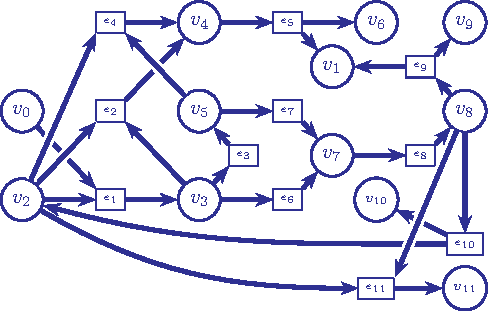
\includegraphics[scale=1.0]{graphics/chapter1/sample_network.pdf}
    \caption{A hypergraph representation of the reactions in the concurrent system.}
    \label{fig:sample_network}
\end{figure}

\begin{figure}[!h]
	\centering
	\vspace{1cm}
	\begin{subfigure}{\textwidth}
		\centering
		\begin{tiny}
		\textcolor{Blue}{
		\begin{tabular}{ccc}
			 \chemfig{HO-[:30]-[:-30]~[:-30]N} $\xrightarrow{+\chemfig{H_2O}}$ &\chemfig{HO-[:-30]-[:30](-[:90]OH)=[:-30]NH} $\xrightarrow{\text{taut.}}$ &\chemfig{HO-[:-30]=[:30](-[:90]OH)-[:-30]NH_2}\\
			 $\xrightarrow{\text{taut.}}$ \chemfig{O=[:-30]-[:30](-[:90]OH)-[:-30]NH_2} & $\xrightarrow{-\chemfig{NH_3}}$ \chemfig{O=[:-30]-[:30]=[:-30]O}
		\end{tabular}}
		\end{tiny}
		\caption{sequence of reactions forming glyoxal from glycolonitrile}
		\label{tab:sample_path1}
    \end{subfigure}
    \\
    \vspace{0.5cm}
    \begin{subfigure}{\textwidth}
    	\centering
    	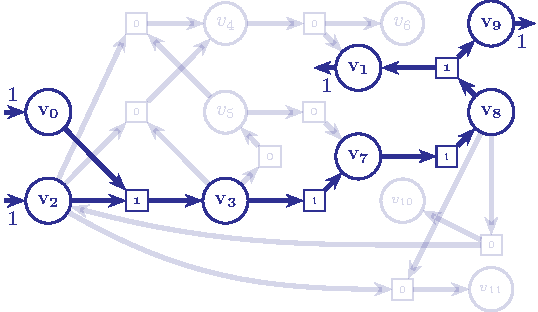
\includegraphics[scale=1.0]{graphics/chapter1/sample_path1.pdf}
    	\caption{A pathway in a hypergraph with the queried molecules $v_9$. The number in the squares denote the number of times the reaction is used to carry out the transformation or the flow assigned to the corresponding hyperedge.}
    	\label{fig:sample_path1}
	\end{subfigure}
	\vspace{0.4cm}
    \caption{The hyperflow denoting the pathway from Figure~\ref{tab:sample_path1} is shown in the hypergraph from Figure~\ref{fig:sample_network}.}
    \label{fig: samplePath1}
\end{figure}
\newpage

We would represent each reaction by a separate hyperedge and each class of molecules by a distinct vertex. This results in the structure shown in Figure~\ref{fig:sample_network}.
The reverse reactions are omitted from the hypergraph in Figure~\ref{fig:sample_network} to reduce clutter. However, in our actual modeling, we do add separate hyperedges to represent the forward and backward directions of reversible reactions.

This data structure representing the concurrent set of reactions in the system is called a multi-directed hypergraph or for simplicity, just a hypergraph. An advantage of using this data structure is that is faithfully represents the many-to-many mappings which are present in reactions which are not unimolecular. Contrast this with a simple directed graph containing edges which map one vertex to another vertex, which are often used to represent and study diverse networks in many situations. The hypergraph in Figure~\ref{fig: hypergraph} is an abstraction of another system of concurrent reactions.

One observes that glyoxal is represented as vertex $v_9$ in the hypergraph. One might query, how one inside this hypergraph can find a pathway producing glyoxal while using the input molecules $v_0$ and $v_2$. One possible transformation pathway is shown in Scheme~\ref{tab:sample_path1}.

Highlighting the hyperedges used in this transformation pathway in the hypergraph results in Figure~\ref{fig:sample_path1}. This sequence of reactions in a pathway can be found by formulating it as a flow query with molecules $v_0$ and $v_2$ as the source molecules and $v_9$ as the target molecule. The ILP assigns integers to the hyperedges which denote the number of times the hyperedge is used in the pathway. Since the flows assigned to the hyperedges are constrained to be integers, this is called an integer hyperflow. The motivation behind using allowing only non-negative integers as permissible hyperflows on a hyperedge is discussed in Section~\ref{sec: discussions}.

Often, there might exist alternative solutions to the flow query. In this case, there exists another valid integer hyperflow to the same flow query in the network with molecules $v_0$ and $v_2$ as the source molecules and $v_9$ as the target molecule which is shown in Figure~\ref{fig:sample_path2}

\begin{figure}[!t]
    \centering
    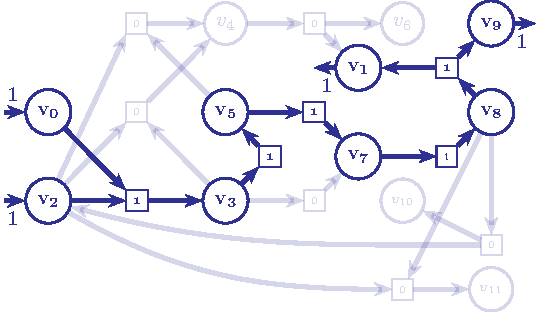
\includegraphics[scale=1.0]{graphics/chapter1/sample_path2.pdf}
    \caption{An alternative pathway to the same flow query as in Figure~\ref{fig:sample_path1}.}
    \label{fig:sample_path2}
\end{figure}

It might so happen than the reaction $v_3 \rightarrow v_7$ is slow (because it has a high energy barrier) and the two step process $v_3 \rightarrow v_5 \rightarrow v_7$ is faster. To judge which of the two pathways is better, a score is assign to them by evaluating an objective function (expression \eqref{proposed_objective} is used in this work) on the pathway, and the one with a better score is ranked higher. This automated search for pathways in a reaction system represented as a hypergraph is the motivation behind introducing the formalism of integer hyperflows in Chapter~\ref{ch:toolbox}.

\section{Generation of Reaction networks}
\label{second appendix}

There exists a diverse range of reactions. However, they are often grouped together on the basis of their mechanisms to create classes of reactions. Reactions in a class share some properties: the reactive core (type of atoms taking part in the reaction), the bonds that are broken, the movement of elections, and the new bonds that are formed. We choose to represent these classes of reactions using reaction templates. Each template defines a change in the bondset of the molecules that take part in the reaction.

For example, in the list of reaction depicted in the hypergraph~\ref{fig:sample_network}:
\begin{itemize}
    \item reactions $e_3$, $e_5$, $e_6$ $e_7$ and $e_8$ have a 1,3-shift of a hydrogen atom (often called tautomerism).
    \item reactions $e_2$, $e_4$ and $e_{11}$ are additions to an trigonal planar carbon to produce a tetrahedral carbon.
    \item reactions $e_9$ and $e_{10}$ eliminate a small molecule from a carbon with two or more adjacent electronegative atoms to form a trigonal planar carbon.
    \item reaction $e_1$ is an addition to a linear carbon to produce a trigonal carbon.
\end{itemize}
Some might prefer more fine-grained reaction templates. For instance, one might define separate templates for keto-enol tautomerism, amide-iminol tautomerism or imine-enamine tautomerism, and similarly for addition to a trigonal planar carbonyl carbon atom and addition to a trigonal planar imine carbon atom. However, that is simply a question of the level of abstraction that the user chooses to work with.

\subsection{Graph transformation rules}
We choose to represent molecules using undirected labeled graphs (hereafter called molecular graphs). The nodes in the graph represent atoms labeled by the symbol of the element, and can carry attributes such as the charge on the atom. The edges in the graph represent bonds labeled by the bond type (single, double, triple or aromatic). with this representation of molecules, the reaction templates used to abstract reactions become graph transformation rules.

A graph transformation rule consists of a subgraph on the left side which can be replaced by the subgraph on the right side when a match of the left-hand side is found in an already existing molecular graph in the network. In other words, the rule converts a part of the graph (representing a fragment of a molecule) and performs a chemical reaction. Let's consider the exchange of hydrogen atoms between oxygen atoms in a carboxylic acid.

\begin{center}
\begin{tiny}
\textcolor{Blue}{
\begin{tabular}{ccc}
     \chemfig{HO-[:30]([:90]=O)-[:-30]R} &$\rightarrow$ &\chemfig{O=[:30]([:90]-OH)-[:-30]R} 
\end{tabular}}
\end{tiny}
\end{center}

The graph transformation rule for this class of reactions would be:
\begin{center}
    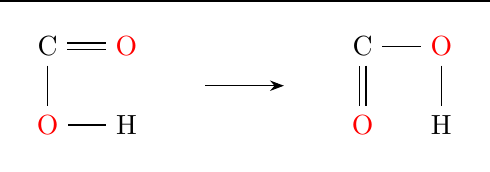
\begin{tikzpicture}[scale=1.0]    
        \tikzset{
            arrow/.style = {->, -{Stealth[length = 5pt]}},
            bond/.style={line width=0.6pt},
            dbond/.style={double, double distance=2pt}
        }
        % vertices
        \node (c0) at (0,0) {C};
        \node (o1) at (1,0) {\textcolor{red}{O}};
        \node (o2) at (0,-1) {\textcolor{red}{O}};
        \node (h3) at (1,-1) {H};
        \draw[bond] (c0) to (o2);
        \draw[bond] (o2) to (h3);
        \draw[dbond] (c0) to (o1);

        \draw[arrow] (2,-0.5) to (3,-0.5);

        \node (c0) at (4,0) {C};
        \node (o1) at (5,0) {\textcolor{red}{O}};
        \node (o2) at (4,-1) {\textcolor{red}{O}};
        \node (h3) at (5,-1) {H};
        \draw[dbond] (c0) to (o2);
        \draw[bond] (o1) to (h3);
        \draw[bond] (c0) to (o1);
    \end{tikzpicture}
\end{center}

The amide-iminol conversion is a more substantial example.
\begin{center}
\begin{tiny}
\textcolor{Blue}{
\begin{tabular}{ccc}
     \chemfig{H_2N-[:30]([:90]=O)-[:-30]R} &$\rightarrow$ &\chemfig{HN=[:30]([:90]-OH)-[:-30]R} 
\end{tabular}}
\end{tiny}
\end{center}

The graph transformation rule for this class of reactions would be:
\begin{center}
    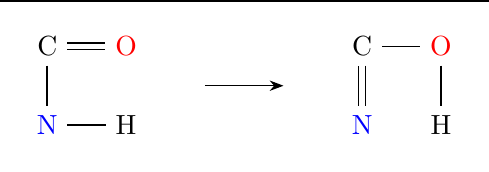
\begin{tikzpicture}[scale=1.0]    
        \tikzset{
            arrow/.style = {->, -{Stealth[length = 5pt]}},
            bond/.style={line width=0.6pt},
            dbond/.style={double, double distance=2pt}
        }
        % vertices
        \node (c0) at (0,0) {C};
        \node (o1) at (1,0) {\textcolor{red}{O}};
        \node (n2) at (0,-1) {\textcolor{blue}{N}};
        \node (h3) at (1,-1) {H};
        \draw[bond] (c0) to (n2);
        \draw[bond] (n2) to (h3);
        \draw[dbond] (c0) to (o1);

        \draw[arrow] (2,-0.5) to (3,-0.5);

        \node (c0) at (4,0) {C};
        \node (o1) at (5,0) {\textcolor{red}{O}};
        \node (n2) at (4,-1) {\textcolor{blue}{N}};
        \node (h3) at (5,-1) {H};
        \draw[dbond] (c0) to (n2);
        \draw[bond] (o1) to (h3);
        \draw[bond] (c0) to (o1);
    \end{tikzpicture}
\end{center}
This rule rewrites an amide fragment when it is found in a molecule with an iminol fragment, thus effecting the required reaction.

For a keto-enol tautomerism like
\begin{center}
\begin{tiny}
\textcolor{Blue}{
\begin{tabular}{ccc}
     \chemfig{R'-[:-30](-[:-90]H)-[:30]([:90]=O)-[:-30]R} &$\rightarrow$ &\chemfig{R'-[:-30]=[:30]([:90]-OH)-[:-30]R} 
\end{tabular}}
\end{tiny}
\end{center}

the graph transformation rule for this class of reactions would be:
\begin{center}
    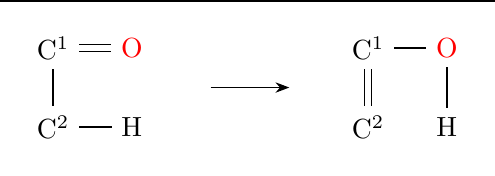
\begin{tikzpicture}[scale=1.0]    
        \tikzset{
            arrow/.style = {->, -{Stealth[length = 5pt]}},
            bond/.style={line width=0.6pt},
            dbond/.style={double, double distance=2pt}
        }
        % vertices
        \node (c0) at (0,0) {C$^1$};
        \node (o1) at (1,0) {\textcolor{red}{O}};
        \node (c2) at (0,-1) {C$^2$};
        \node (h3) at (1,-1) {H};
        \draw[bond] (c0) to (c2);
        \draw[bond] (c2) to (h3);
        \draw[dbond] (c0) to (o1);

        \draw[arrow] (2,-0.5) to (3,-0.5);

        \node (c0) at (4,0) {C$^1$};
        \node (o1) at (5,0) {\textcolor{red}{O}};
        \node (c2) at (4,-1) {C$^2$};
        \node (h3) at (5,-1) {H};
        \draw[dbond] (c0) to (c2);
        \draw[bond] (o1) to (h3);
        \draw[bond] (c0) to (o1);
    \end{tikzpicture}
\end{center}
Note that the graph transformation rule indicates the bare minimum that is required to be present as a subgraph in the molecule for the reaction to occur. For example, the carbon at the 2-position, might have two adjacent hydrogen atoms, but the rule specifies that at least one hydrogen atom is required for the keto isomer to convert into the enol isomer. Without any hydrogen at the 2-position, the fragment on the left is not a subgraph of the molecule and this transformation rule cannot be applied to the graph.

Also, note that the objective here is not to capture the exact mechanism of the reaction, but rather specify what the molecular fragment is before and after the reaction. In all the three reactions mentioned above, the 1,3-hydrogen transfer involves a solvent molecule. In most cases, it is not the exact same hydrogen atom that would be in the molecule before and after the reaction.

The similarity in the graph transformation rule for the three reactions mentioned above above look similar. For a more elegant formulation, we define the following graph transformation rule to account for all the three cases above:
\begin{center}
    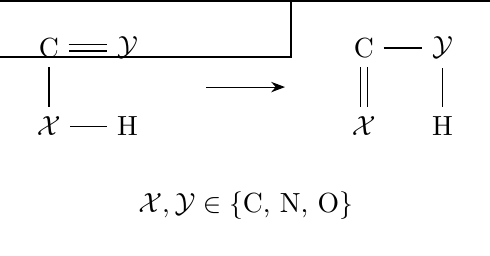
\begin{tikzpicture}[scale=1.0]    
        \tikzset{
            arrow/.style = {->, -{Stealth[length = 5pt]}},
            bond/.style={line width=0.6pt},
            dbond/.style={double, double distance=2pt}
        }
        % vertices
        \node (c0) at (0,0) {C};
        \node (o1) at (1,0) {$\mathcal{Y}$};
        \node (c2) at (0,-1) {$\mathcal{X}$};
        \node (h3) at (1,-1) {H};
        \draw[bond] (c0) to (c2);
        \draw[bond] (c2) to (h3);
        \draw[dbond] (c0) to (o1);

        \draw[arrow] (2,-0.5) to (3,-0.5);

        \node (c0) at (4,0) {C};
        \node (o1) at (5,0) {$\mathcal{Y}$};
        \node (c2) at (4,-1) {$\mathcal{X}$};
        \node (h3) at (5,-1) {H};
        \draw[dbond] (c0) to (c2);
        \draw[bond] (o1) to (h3);
        \draw[bond] (c0) to (o1);

        \node at (2.5,-2) {$\mathcal{X}, \mathcal{Y} \in \{\text{C, N, O}\}$};
    \end{tikzpicture}
\end{center}

This graph transformation rule also encodes an allyl hydrogen shift, an imine-enamine tautomerism, or the hydrogen exchange in amidine.
\begin{center}
\begin{tiny}
\textcolor{Blue}{
\begin{tabular}{ccc}
    \chemfig{R_4-[:-30](-[:120]R_5)(-[:-90]H)-[:30]([:90]-R_3)=[:-30](-[:-90]R_2)-[:30]R_1} &$\rightarrow$ &\chemfig{R_4-[:-30](-[:-90]R_5)=[:30]([:90]-R_3)-[:-30](-[:-90]R_2)(-[:60]H)-[:30]R_1} \\\\
    \chemfig{R'-[:-30](-[:-90]H)-[:30]([:90]=NH)-[:-30]R} &$\rightarrow$ &\chemfig{R'-[:-30]=[:30]([:90]-NH_2)-[:-30]R} \\\\
    \chemfig{H_2N-[:30]([:90]=NH)-[:-30]R} &$\rightarrow$ &\chemfig{HN=[:30]([:90]-NH_2)-[:-30]R} 
\end{tabular}}
\end{tiny}
\end{center}

However, all these six different reactions are expected to have differing mechanisms. This graph transformation rule introduces two variables $\mathcal{X}, \mathcal{Y}$ which can be matched with the label C, N or O, or in other words the atoms in the place of  $\mathcal{X}, \mathcal{Y}$ in the molecular fragment can be a carbon, nitrogen or oxygen atom.

Similarly the graph transformation rule
\begin{center}
    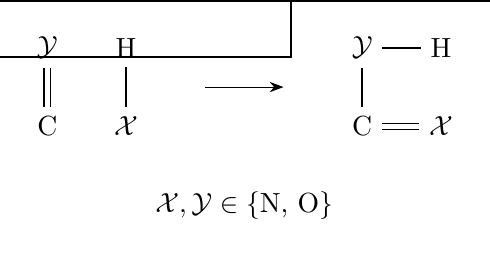
\begin{tikzpicture}[scale=1.0]    
        \tikzset{
            arrow/.style = {->, -{Stealth[length = 5pt]}},
            bond/.style={line width=0.6pt},
            dbond/.style={double, double distance=2pt}
        }
        % vertices
        \node (c0) at (0,-1) {C};
        \node (o1) at (0,0) {$\mathcal{Y}$};
        \node (c2) at (1,-1) {$\mathcal{X}$};
        \node (h3) at (1,0) {H};
        \draw[bond] (c2) to (h3);
        \draw[dbond] (c0) to (o1);

        \draw[arrow] (2,-0.5) to (3,-0.5);

        \node (c0) at (4,-1) {C};
        \node (o1) at (4,0) {$\mathcal{Y}$};
        \node (c2) at (5,-1) {$\mathcal{X}$};
        \node (h3) at (5,0) {H};
        \draw[dbond] (c0) to (c2);
        \draw[bond] (o1) to (h3);
        \draw[bond] (c0) to (o1);

        \node at (2.5,-2) {$\mathcal{X}, \mathcal{Y} \in \{\text{N, O}\}$};
    \end{tikzpicture}
\end{center}

encodes the addition of a water or ammonia molecule to a carbonyl or imine group.
\begin{center}
\begin{tiny}
\textcolor{Blue}{
\begin{tabular}{ccc}
    \chemfig{R'-[:30]([:90]=NH)-[:-30]R} &$\xrightarrow{+\chemfig{NH_3}}$ &\chemfig{R'-[:30]([:90]-NH_2)(-[:-60]NH_2)-[:-30]R} \\\\
    \chemfig{R'-[:30]([:90]=NH)-[:-30]R} &$\xrightarrow{+\chemfig{H_2O}}$ &\chemfig{R'-[:30]([:90]-NH_2)(-[:-60]OH)-[:-30]R} \\\\
    \chemfig{R'-[:30]([:90]=O)-[:-30]R} &$\xrightarrow{+\chemfig{NH_3}}$ &\chemfig{R'-[:30]([:90]-OH)(-[:-60]NH_2)-[:-30]R} \\\\
     \chemfig{R'-[:30]([:90]=O)-[:-30]R} &$\xrightarrow{+\chemfig{H_2O}}$ &\chemfig{R'-[:30]([:90]-OH)(-[:-60]OH)-[:-30]R} 
\end{tabular}}
\end{tiny}
\end{center}
We admit that these reactions are not a simple one step process as the transformation rule make them appear to be and not all of these possible reactions is always feasible for all reactant molecules.

In all the graph transformation rules in this section, the context graph $K$, which comes between the left and right-hand sides, is omitted. The context graph must be added to the graph transformation rules for mathematical correctness. It ensures that logically the bonds are first removed, and then added, making the graph rewriting a two-step process.

\subsection{Rule application to a graph}

When a graph transformation rule is applied to a set of reactant molecules, a reaction might occur. First, it is checked if the left-hand side of the rule, $L$, is present as a subgraph in the set of reactant molecules $G$. If so, then that subgraph is rewritten according to the rule to R, to generate a new set of molecules $H$, the product molecules. This process is illustrated in Figure~\ref{fig:rule_application1}.

\begin{figure}[!t]
    \centering
    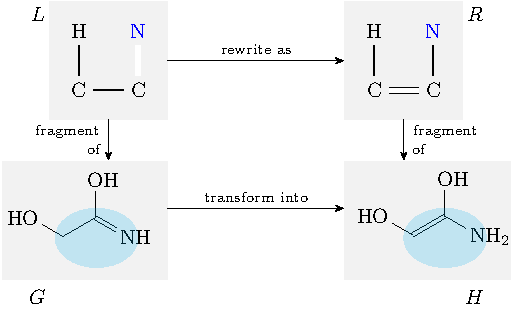
\includegraphics[width=\linewidth]{graphics/chapter1/rule_app1.pdf}
    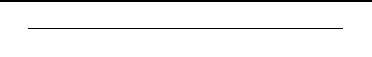
\begin{tikzpicture}
        \draw (0, 0) -- (4, 0);
    \end{tikzpicture}
    \vspace{1.0cm}\\
    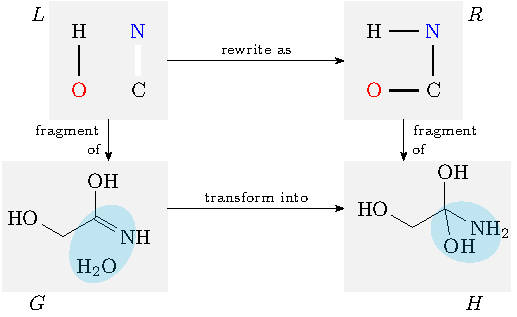
\includegraphics[width=\linewidth]{graphics/chapter1/rule_app2.pdf}
    \caption{Two examples of the application of a graph transformation rule to a collection of molecules.}
    \label{fig:rule_application1}
\end{figure}

If the left-hand side of the rule, $L$, is not present in the set of molecules $G$, then that reaction template cannot be applied to the given set of molecules.

\begin{figure}[h]
    \centering
    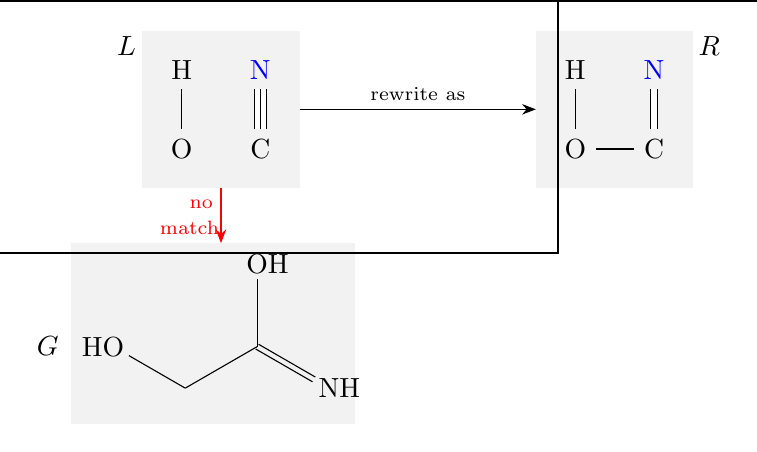
\begin{tikzpicture}[scale=1.0]    
        \tikzset{
            arrow/.style = {->, -{Stealth[length = 5pt]}},
            bond/.style={line width=0.6pt},
            dbond/.style={double, double distance=2pt},
            tbond/.style={double, double distance=4pt}
        }
        % vertices
        \draw[fill=gray, fill opacity=0.1, draw=none] (-0.5,-0.5) rectangle (1.5,1.5);
        \node at (-0.7, 1.3) {$L$};
        \node (c0) at (1,0) {C};
        \node (n1) at (1,1) {\textcolor{blue}{N}};
        \node (c2) at (0,0) {O};
        \node (h3) at (0,1) {H};
        \draw[bond] (c2) to (h3);
        \draw[tbond] (c0) to (n1);
        \draw[bond] (c0) to (n1);
        
        \draw[arrow] (1.5,0.5) to (4.5,0.5);
        \node at (3,0.7) {\scriptsize{rewrite as}};

        \draw[fill=gray, fill opacity=0.1, draw=none] (4.5,-0.5) rectangle (6.5,1.5);
        \node at (6.7, 1.3) {$R$};
        \node (c0) at (6,0) {C};
        \node (n1) at (6,1) {\textcolor{blue}{N}};
        \node (c2) at (5,0) {O};
        \node (h3) at (5,1) {H};
        \draw[bond] (c2) to (h3);
        \draw[bond] (c0) to (c2);
        \draw[dbond] (c0) to (n1);

        \draw[fill=gray, fill opacity=0.1, draw=none] (-1.4,-3.5) rectangle (2.2,-1.2);
        \node (lhs) at (0.5, -2.25) {\chemfig{HO-[:-30]-[:30](-[:90]OH)=[:-30]NH}};
        \node at (-1.7,-2.5) {$G$};
        
        \draw[arrow, color=red] (0.5,-0.5) to (0.5,-1.2);
        \node at (0.25,-0.7) {\scriptsize{\textcolor{red}{no}}};
        \node at (0.1,-1) {\scriptsize{\textcolor{red}{match}}};
    \end{tikzpicture}
    \caption{A case where the graph transformation rule cannot be applied to a molecule}
    \label{fig:rule_application2}
\end{figure}
Therefore, the application of a rule to an existing set of molecules might produce new molecules, which in turn expands the molecular space. Repeated application of these rules constructs a network, which is detailed in the next section.

\subsection{Construction of the reaction network}

The construction of the reaction network requires a set of input molecules and some graph transformation rules. A match between a collection of molecules and the subgraph on the left-hand side of one of the transformation rules means that this reaction template can be applied to that collection of molecules created from the input set of molecules. Thus, when a rule is applied to a collection of molecules from the current set of molecules, new molecules are created. In a generative process, these new molecules are then added to the set of available molecules (i.e., this set is updated). Graph transformation rules can be recursively applied to this new set of molecules, effecting more reactions to be made and thus the molecular space expands. The hypergraph representation of the network keeps track of all the reactions performed and of the molecules current present in the network.

\begin{figure}
    \centering
    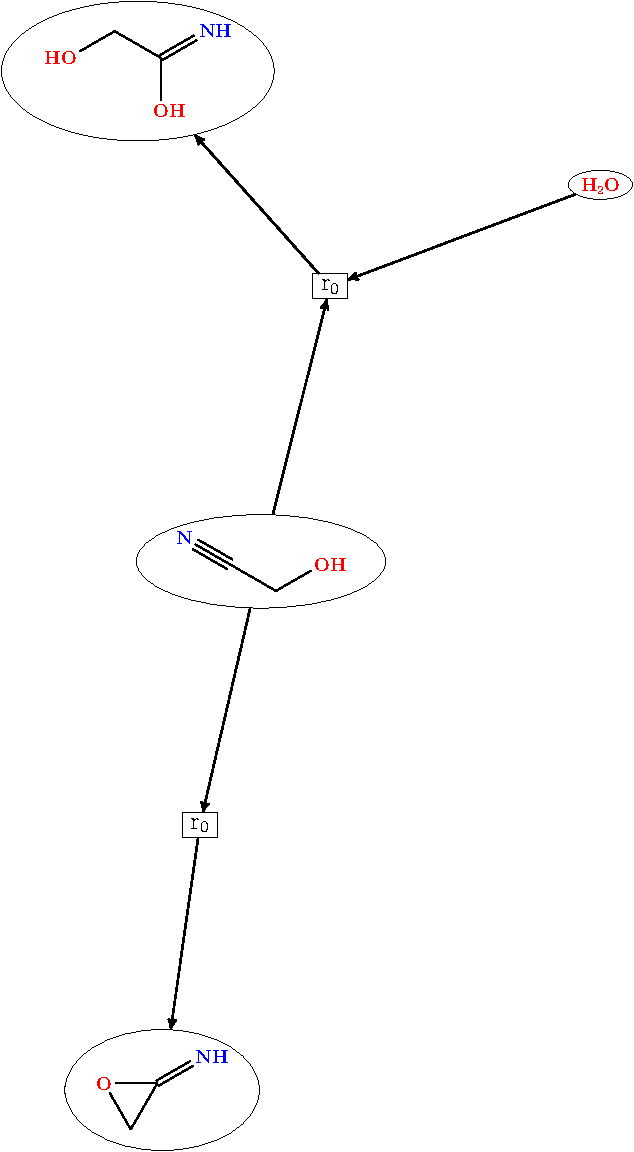
\includegraphics[scale=0.3]{graphics/chapter1/recurse1.pdf}\\
    \vspace{0.4cm}
    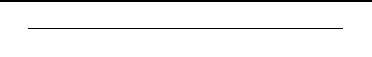
\begin{tikzpicture}
        \draw (0, 0) -- (4, 0);
    \end{tikzpicture}\\
    \vspace{1.0cm}
    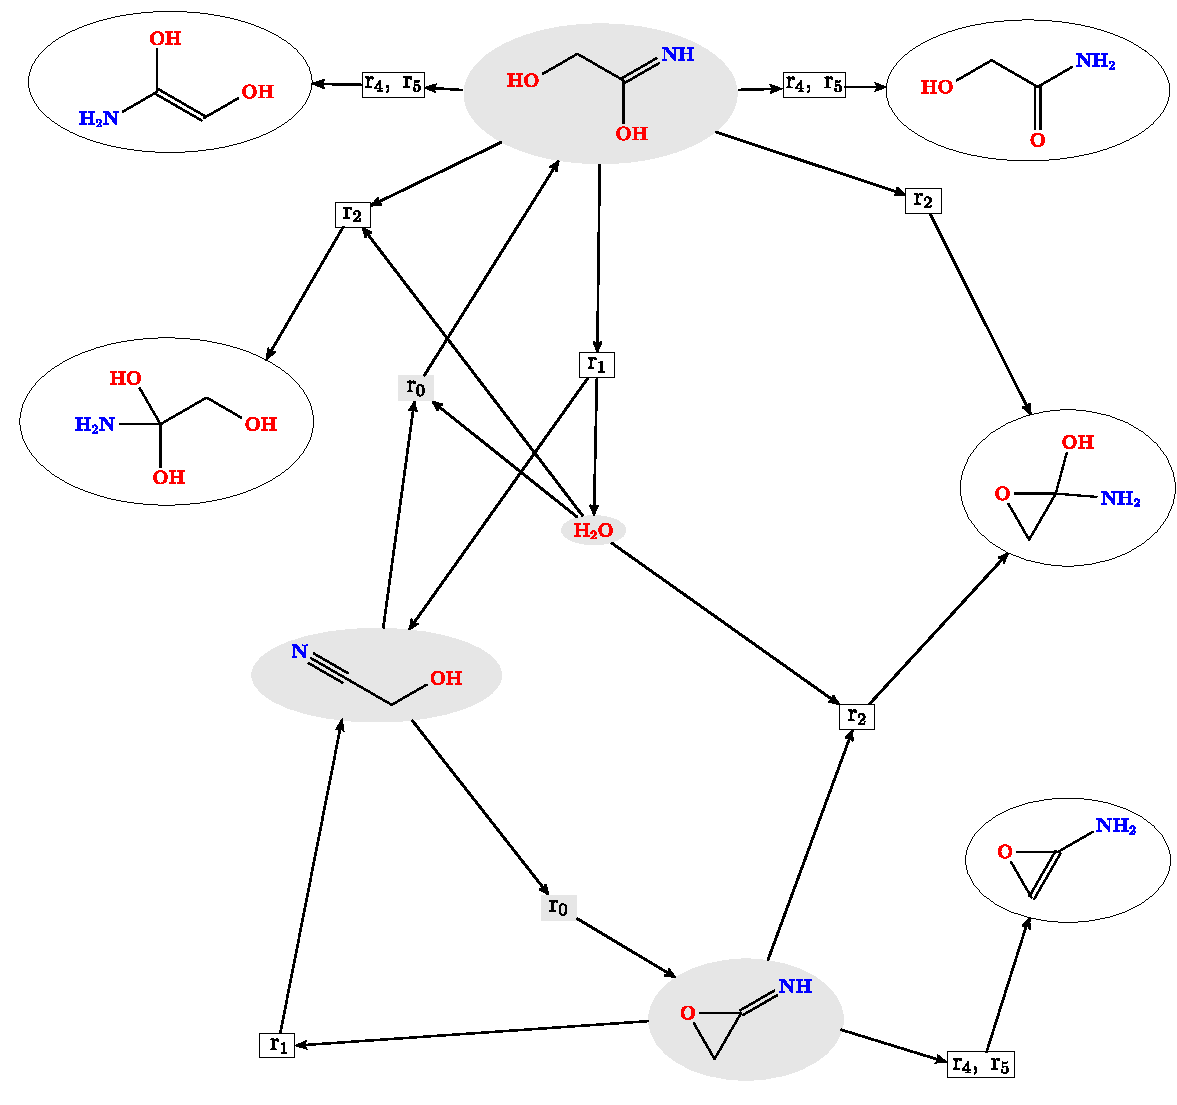
\includegraphics[scale=0.4]{graphics/chapter1/recurse2.pdf}
    \vspace{0.5cm}
    \caption{(top) The reaction network (with $4$ molecules and $2$ reactions) after one recursive application of the graph transformation rules, and (bottom) the reaction network (with $9$ molecules and $10$ reactions) after two recursive applications of the graph transformation rules. The part of the network already generated previously has been shaded.}
    \label{fig: grow_network}
\end{figure}

\begin{figure}
    \centering
    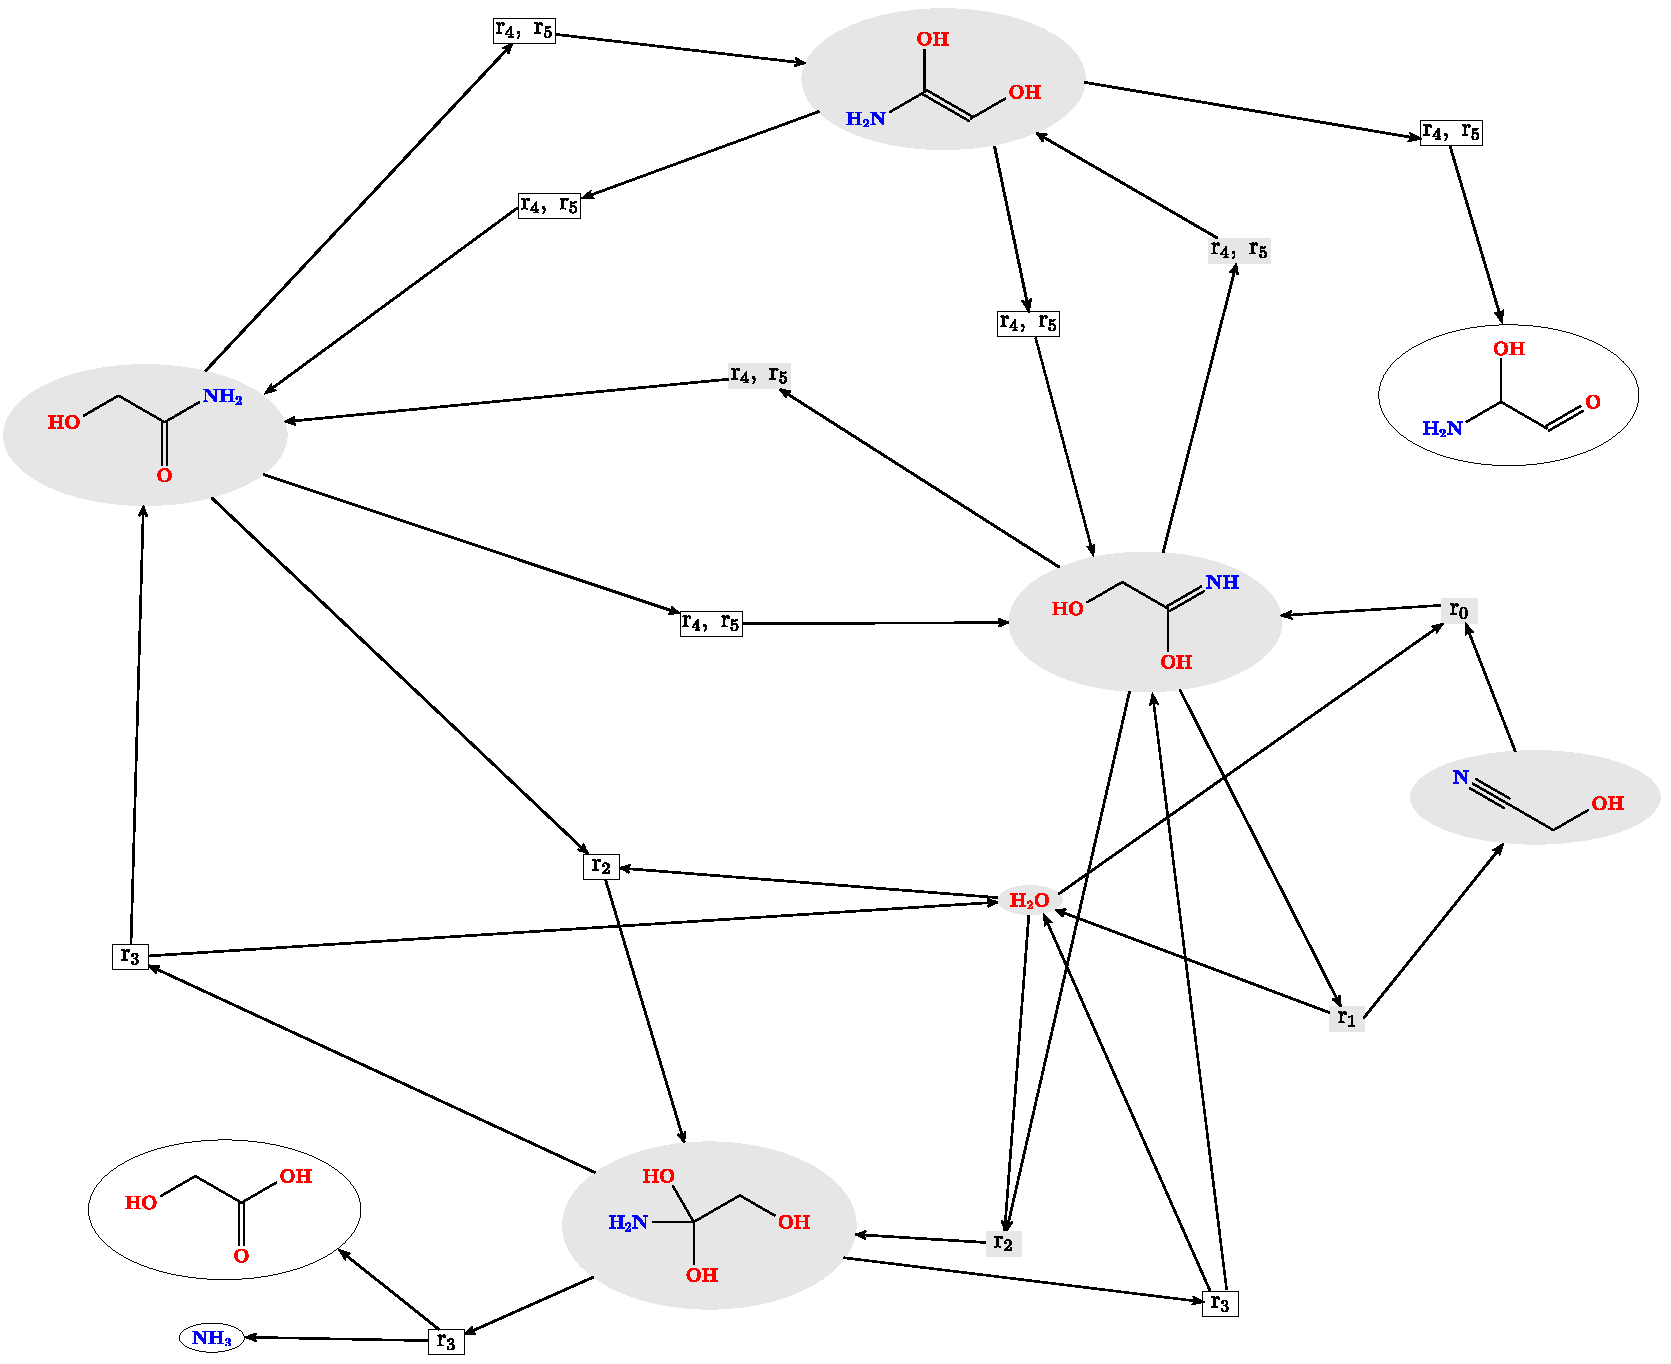
\includegraphics[width=\linewidth]{graphics/chapter1/recurse3.pdf}
    \vspace{0.5cm}
    \caption{The reaction network (with $9$ molecules and $14$ reactions) after three recursive applications of the graph transformation rules with the 3-cycles filtered out. The part of the network already generated previously has been shaded.}
    \label{fig: recurse3}
\end{figure}

To illustrate the construction of a reaction network by the recursive application of graph transformation rules to an input set of molecules, the graph transformation rules from Figure~\ref{fig:graphTransformationRules} in Chpater~\ref{ch:casestudy2} is applied to the input molecules water and 2-hydroxyethanenitrile is shown in Figures~\ref{fig: grow_network}, \ref{fig: recurse3} and \ref{fig: recurse4}.

Notice that some molecules in Figure~\ref{fig: grow_network}, such as the 3-cycles, are not realistic. One can disallow their addition to the generated reaction network by using so-called right predicates. Right predicates filter out certain reactions from the network based on the properties of the molecular graphs that appear on the right-hand side of a derivation. This, it prunes the generated network and makes its growth more manageable and potentially more realistic. The effect of using the right predicate can be seen in the hypergraph in Figure~\ref{fig: recurse3}, which has $9$ molecules after three recursive expansion steps, while the hypergraph in Figure~\ref{fig: grow_network} already had $9$ molecules after two recursive steps when the right predicate was not used.

\begin{figure}
    \centering
    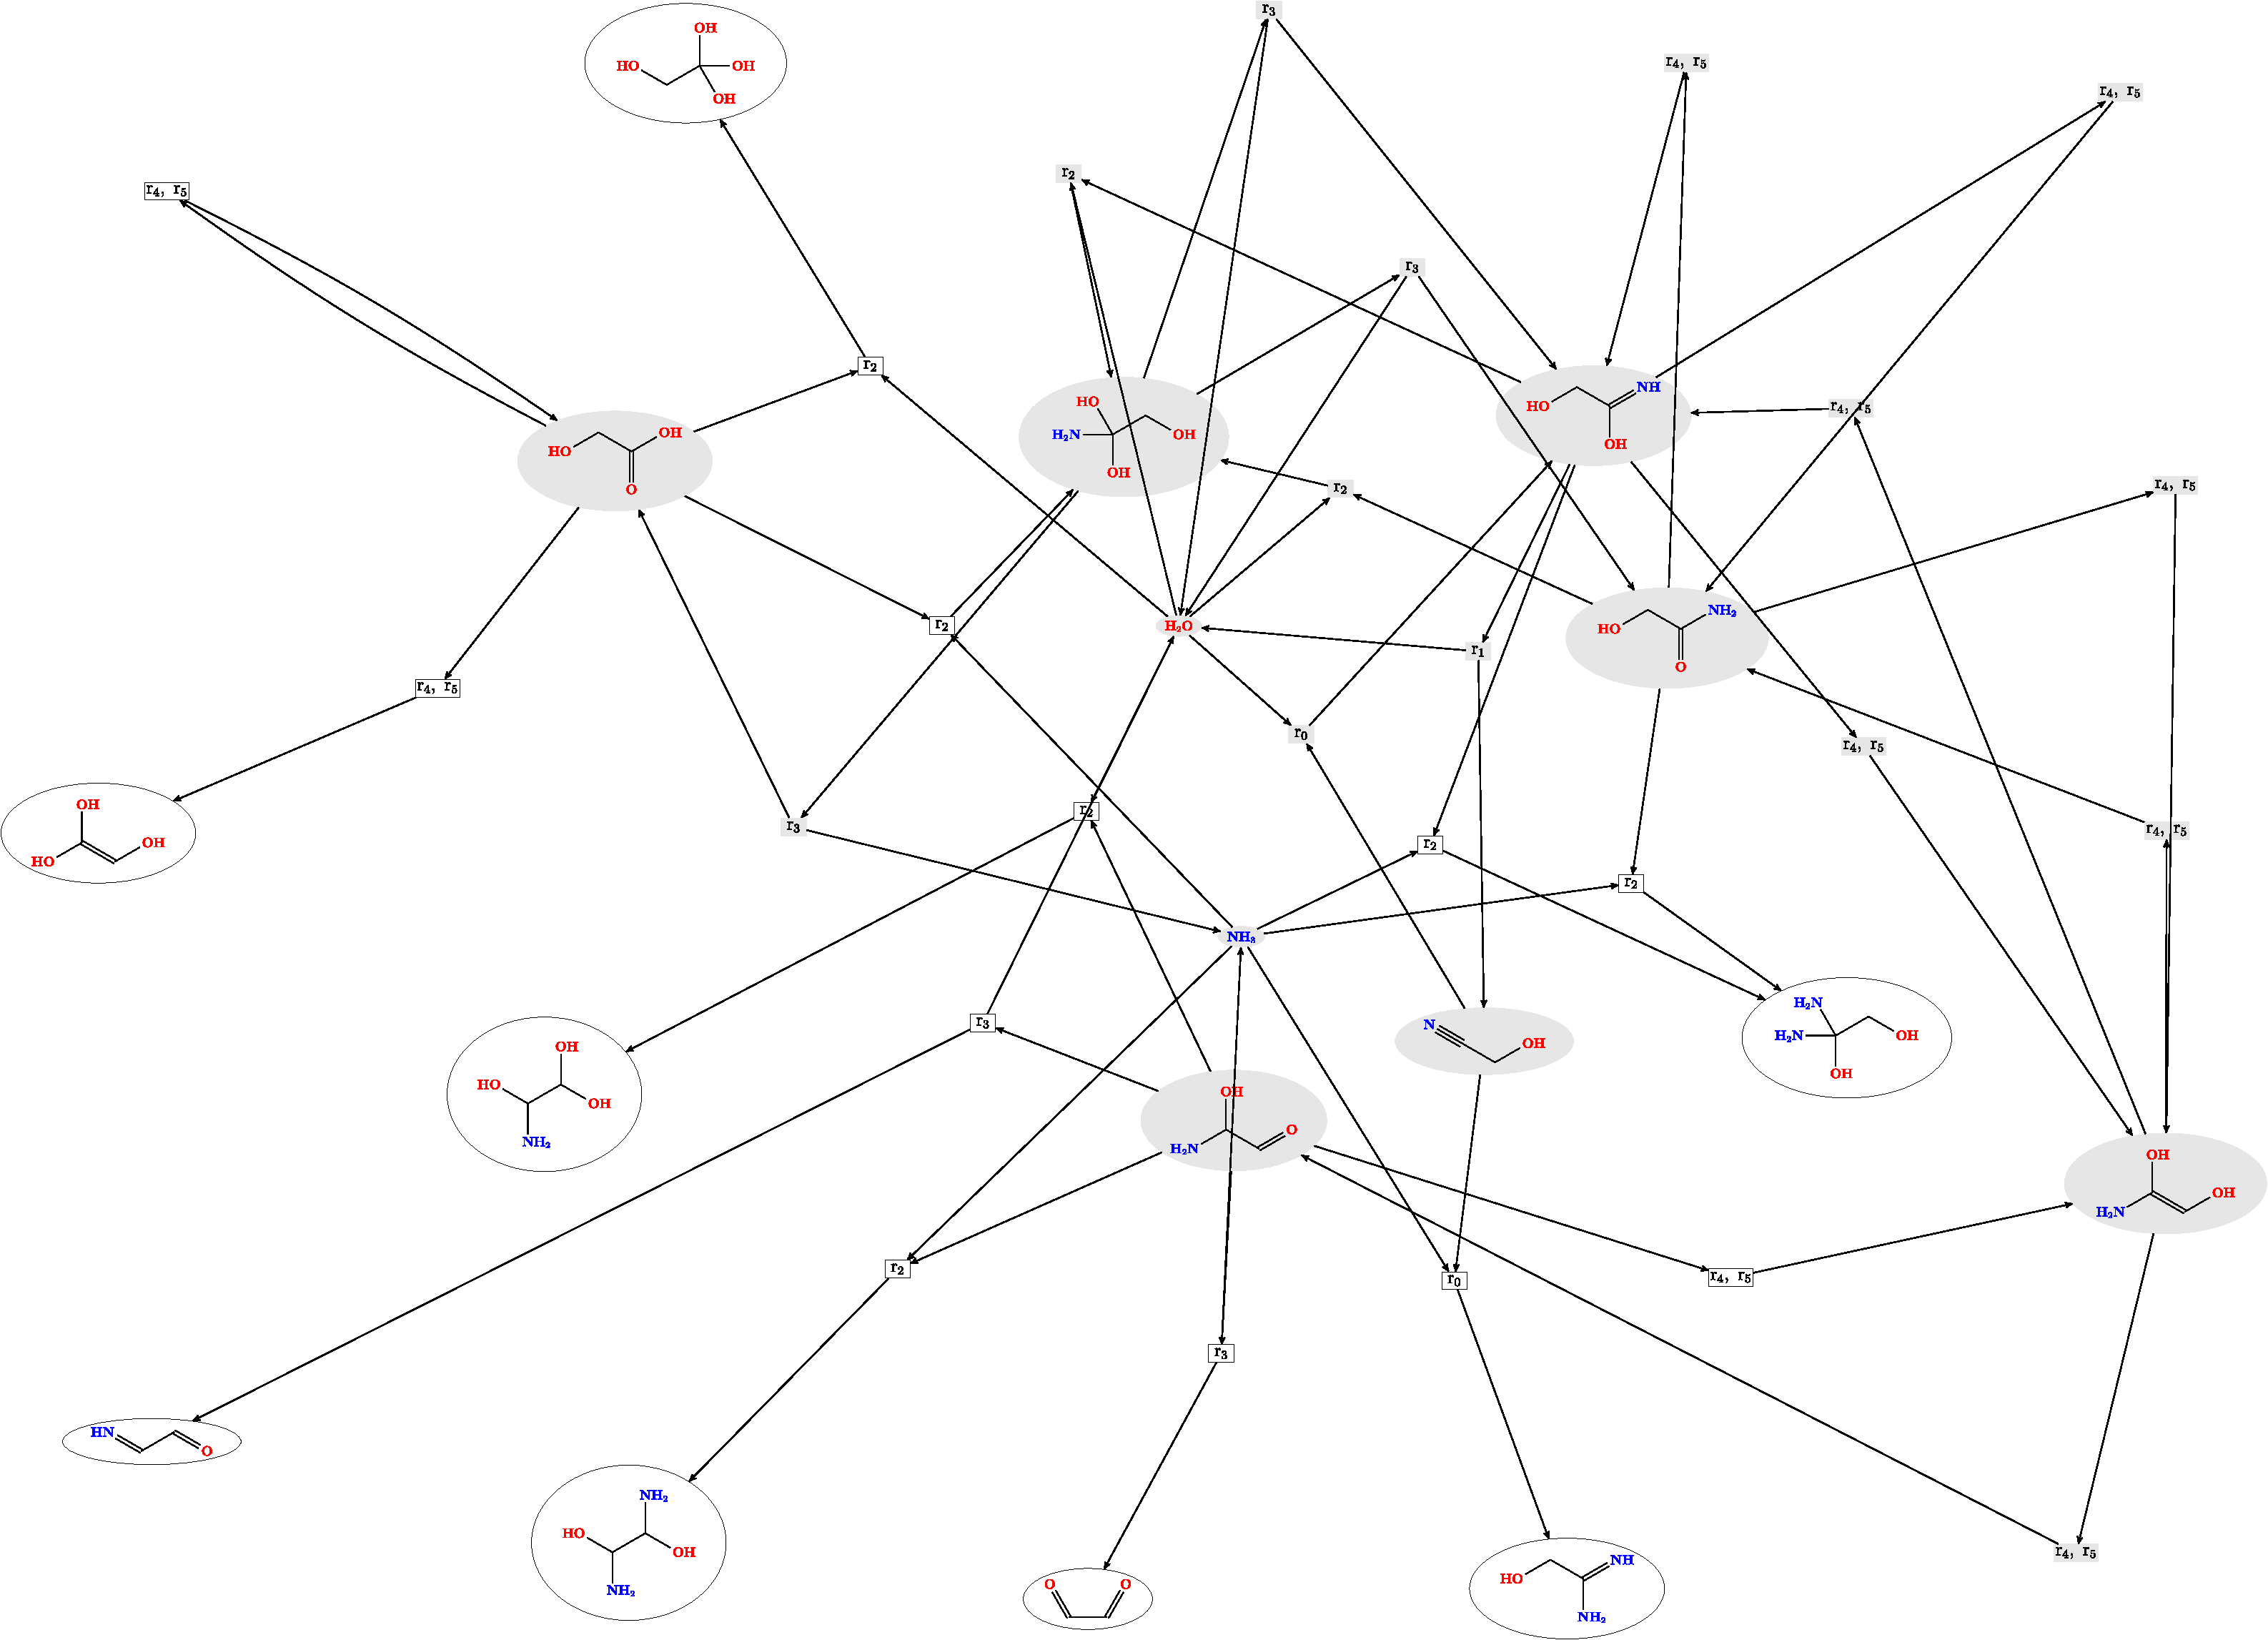
\includegraphics[width=\linewidth]{graphics/chapter1/recurse4.pdf}
    \vspace{0.5cm}
    \caption{The reaction network (with $17$ molecules and $26$ reactions) after four recursive applications of the graph transformation rules with the 3-cycles filtered out. The part of the network that was already generated aftre three recersive steps has been shaded.}
    \label{fig: recurse4}
\end{figure}

Often, one direction of a reaction is added to the hypergraph (adding new molecules to the existing set of molecules) and the reverse direction is added in the next recursion. This adds a new reaction between reactants and products both of which are already present in the set of existing molecules.
The graph transformation rules can be applied for a specified number of iterations, or until a specified limit on the size of the different molecules generated is reached which terminated the network generation process. This makes the derived hypergraph finite.

\section{Hyperflows and Fluxes}
\label{sec: comparison}

In this section, we give a comparison of our workflow with existing methods. Constraint-based models such as flux balance analysis also use constraint programming with an objective function that is optimized. For instance, open-source tools such as COBRApy~\cite{cobrapy} perform flux analysis on a reaction network supplied to them. However, such tools do not construct the network on the fly in a generative way--- rather the reaction network has to be constructed beforehand using some other tool. Flux balance analysis generates a flux vector for the reactions in the network which is allowed to contain floating-point values, while our method accepts only integers as a valid hyperflow for a reaction, which is more aligned with the standard notion of a pathway. Formulating a flux balance analysis on the network would be equivalent to an LP relaxation of the pathway query problem using integer hyperflows for the same network. A linear program (LP) can be solved in polynomial time while an ILP is NP-hard. However, formulating the search for pathways to a queried molecule in a reaction network offers some advantages.

\begin{figure}
    \centering
    \begin{subfigure}{\textwidth}
        \centering
        \includegraphics[scale=1.0]{graphics/chapter1/example_network.pdf}
        \vspace{0.4cm}
        \caption{An example reaction network with $4$ molecules and $3$ reactions.}
        \label{fig:example_network}
    \end{subfigure}\\
    \vspace{0.8cm}
    \begin{subfigure}{\textwidth}
        \centering
        \includegraphics[scale=1.0]{graphics/chapter1/example_flux.pdf}
        \vspace{0.4cm}
        \caption{A flux distribution in the network which produces an outflow of $1.5$ for $v_3$.}
        \label{fig:example_flux}
    \end{subfigure}\\
    \vspace{0.8cm}
    \begin{subfigure}{\textwidth}
        \centering
        \includegraphics[scale=1.0]{graphics/chapter1/example_flow.pdf}
        \vspace{0.4cm}
        \caption{An assignment of integer hyperflows in the network which produces an outflow of $1$ for $v_3$.}
        \label{fig:example_flow}
    \end{subfigure}
    \vspace{1cm}
    \caption{Comparison of flux balance analysis and an integer hyperflow in an example reaction network.}
    \label{fig:comparison}
\end{figure}

There exists reaction networks where the optimal solutions from the ILP formulated by our modeling and the relaxed LP from flux balance analysis differ. Consider the reaction network shown in Figure~\ref{fig:example_network} with the following formulation of the problem:
\begin{align*}
    &\max \left( \text{outflow}(v_3) \right) \\
    \text{subject to: } &\text{inflow}(v_0) + \text{inflow}(v_1) +\text{inflow}(v_2) \leq 3
\end{align*}
The optimal flux distribution yields an objective value of $1.5$ with the assigned fluxes shown in Figure~\ref{fig:example_flux} while our method assigns the integer hyperflows shown in Figure~\ref{fig:example_flow} in one of the three optimal solutions with objective value $1$. The other two solutions assign the hyperflows $(0,1,1)$ and $(1,1,0)$ to the hyperedge set $(e_1,e_2,e_3)$ respectively.

The ILP solution space is a subset of the LP feasible reaction and therefore, the objective value for the optimal solution for the relaxed LP will always be as at least as large as the objective value of optimal solution for the corresponding ILP. This is illustrated in the example shown in Figure~\ref{fig:comparison} too. As the result, the fluxes and the structure of the solution is often different from those if they were constrained to be integers.

Restricting hyperflows to integers makes physical sense because molecules occur and react in discrete quantities.
Actually, small molecular counts in several biological settings (often involving trace amounts of enzymes and inhibitors affecting multiple iterations of the same pathway) and physical cases (as in chain reactions and cascades) do not allow arbitrary scaling of the number of molecules, as the use of real-valued fluxes by flux balance analysis assume.
When a small number of molecules are encountered in a scenario as above (or in scenarios with appearances of a rare but significant molecule in the system), the discrete nature of the molecules becomes more pronounced.

Another feature of our proposed method is the enumeration of alternative pathways with disjoint set of hyperedges ranked on the basis of a chosen objective function. While flux balance analysis offers the possibility to find alternative pathways~\cite{fba_alternative_pathways}, they have the same objective value but a different flux distribution in the network. This differs from the enumeration of solutions in the current method which offers a list of pathways ordered by the increasing value of the objective function for the user to choose from. Enumerating solutions over variables with a continuous domain is difficult using indicator variables and biimplications as in constraints \ref{biimp1}  and \ref{biimp2}. The enumeration of solutions offers diverse pathways to the queried molecules and makes the method more robust to uncertainties in the weights assigned to the hyperedges.

\printbibliography[
  heading=subbibliography,
  title={References}
]

\end{refsection}

%************************************************
\chapter[A Constraint-based Model]{Pathways using Thermodynamic Constraints}
\label{ch:thermodynamic_model}
%************************************************

{\sffamily\slshape The text in this chapter is identical to Section 3 of the published version of the preprint at \href{https://arxiv.org/abs/2411.15900}{arXiv:2411.15900} while a number of additional figures were added.\\}

Analogous to typical thermodynamics problems where pathways maximizing the work done by the flow of heat between the system and the reservoir are sought (such as the cycle of a heat engine as shown in Figure~\ref{fig: heatCycles}),
we seek pathways in our system to maximize the chemical work done (interpreted as maximizing the production of the target molecules) by directing the flow of molecules along specific reactions on the free energy landscape.

Classical thermodynamics---contrary to the `dynamics' in the name---is used to study systems at equilibrium,
or near equilibrium, when the thermodynamic driving forces are in exact balance.
In a closed system, the concentrations of the molecules in the system would be such that the chemical potentials of all the molecules in the reaction network is the same.
To achieve the required flow along the pathway returned by our method,
one has to perturb the system from the equilibrium by tweaking the molecular concentrations in a direction returned by the solution.
In practical scenarios, this is done supplying a steady inflow of the source molecules and removing the target molecules from the system to maintain a non-zero thermodynamic driving force along the pathway.  
For perturbations that are small enough, the equations from classical thermodynamics describing the equilibrium situation can still be used as a first-order approximation.
The gradients of the chemical potentials in general, or in our case, the differences in the chemical potentials of the target molecules and the source molecules in a elementary reaction serve as the thermodynamic force driving a reaction.
In the linear regime, the flow for each reaction would be directly proportional to the thermodynamic forces driving the flow.
The forces driving the flows in a reaction network might not remain linear functions of the difference in the chemical potentials farther from the equilibrium, resulting in non-linear dynamics.
Therefore, in this work we would restrict ourselves to analyzing the system perturbed, within acceptable limits,
from the equilibrium, so that using equations from equilibrium thermodynamics does not introduce large errors into the calculations.
\newpage

\begin{figure}[!t]
    \centering
    \begin{subfigure}{0.9\textwidth}
        \centering
        \vspace{0.4cm}
        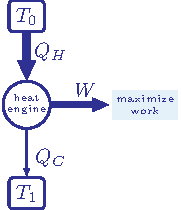
\includegraphics[width=0.4\textwidth]{graphics/chapter2/heatEngine.pdf}
        \vspace{0.5cm}
        \caption{A heat engine attempts to maximize the work done $W = Q_H - Q_C$, while transferring energy in the form of heat between two reservoirs at temperatures $T_0$ and $T_1$, respectively.}
        \label{fig: heatEngine}
    \end{subfigure}
    \\
    \vspace{2cm}
    \begin{subfigure}{0.9\textwidth}
        \centering
        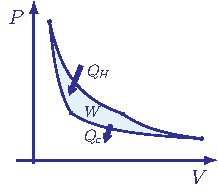
\includegraphics[width=0.5\textwidth]{graphics/chapter2/heatPathway.pdf}
        \vspace{0.5cm}
        \caption{The pathway followed by the heat engine while performing work $W$ is illustrated in the physical $P-V$ space of the system.}
        \label{fig: heatPathway}
    \end{subfigure}
    \vspace{0.5cm}
    \caption{Thermodynamics studied the pathways traversed by heat engines in the $P-V$ space which maximized the work done by it. The efficiency of such heat engines was calculated as $\eta = \frac{W}{Q_H} = \frac{Q_H - Q_C}{Q_H} = 1 - \frac{Q_C}{Q_H}$ which can be shown t be equivalent to $\eta = 1 - \frac{T_1}{T_0}$. therefore, increasing the temperature gradient in the system increased the work done by the heat engine under ideal conditions.}
    \label{fig: heatCycles}
\end{figure}
\newpage

\section{Mathematical Formulation}\label{math_form}

The first step to make the search more realistic is to assign the chemical potentials to the vertices and add constraints which allow only thermodynamically favorable reactions in the returned pathway. 
Chemical potentials are real-valued numbers. 
Hence, the inclusion of customized linear constraints and objective functions involving floating-point variables for the chemical potentials and concentrations of molecules requires us to extend the existing ILP model in M{\O}D to one using MILP incorporating these variables. This is the key focus of the current work.

MILP attempts to model the system with linear inequalities involving some variables (both integer-values and floats, hence mixed) describing the system. An infeasible system of inequalities indicates that there is no solution to the problem under those specific constraints. When a feasible solution space exists, one often attempts to optimize the solution, by maximizing (or minimizing) the value of some objective function. Tn this section, we develop the structure of the MILP model, first with using logical constraints using implications in the next section on the constraint-based model, and later, in in the discussion on implementing them, we linearize it into an MILP that can be solved using a solver.

\begin{figure}[!t]
    \centering
    \vspace{1cm}
    \begin{subfigure}{0.9\textwidth}
        \centering
        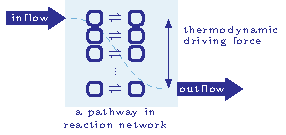
\includegraphics[width=0.75\textwidth]{graphics/chapter2/thermPathway.pdf}
        \vspace{0.5cm}
        \caption{A pathway in a chemical reaction network is a sequence of reactions that convert the source molecules (with supplied inflow) to the target molecules (with required inflow). In a thermodynamically consistent modeling, the pathway would aim to maximize the thermodynamic driving force along the pathway producing the target molecules.}
        \label{fig: thermPathway}
    \end{subfigure}
    \\
    \vspace{2cm}
    \begin{subfigure}{0.9\textwidth}
        \centering
        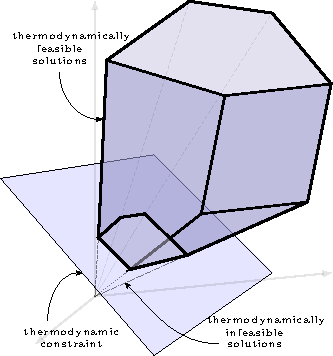
\includegraphics[width=0.55\textwidth]{graphics/chapter2/thermConstraints.pdf}
        \vspace{0.5cm}
        \caption{The addition of constraints describing the thermodynamics of the system prunes the solution space of the system, leading to hyperflow solutions that were valid earlier being thermodynamically infeasible.}
        \label{fig: thermConstraints}
    \end{subfigure}
    \vspace{0.5cm}
    \caption{A thermodynamically informed modeling of pathways in reaction networks requires the addition of constraints based on thermodynamics to capture the energetics in the system. This leads to the modification of the solution space.}
    \label{fig: thermModeling}
\end{figure}

\subsection{Constraint-Based Model}
\label{milp_implication}

\begin{figure}[!t]
    \centering
    \begin{subfigure}{0.4\textwidth}
        \centering
        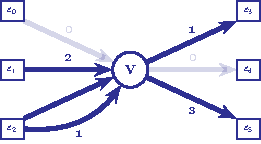
\includegraphics[width=\textwidth]{graphics/chapter2/flowConv1.pdf}
        \caption{}
        \label{fig: flowConv1}
    \end{subfigure}%
    \hfill
    \begin{subfigure}{0.4\textwidth}
        \centering
        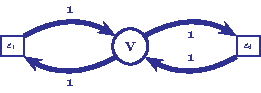
\includegraphics[width=\textwidth]{graphics/chapter2/flowConv4.pdf}
        \caption{}
        \label{fig: flowConv2}
    \end{subfigure}
    \\
    \vspace{1cm}
    \begin{subfigure}{0.4\textwidth}
        \centering
        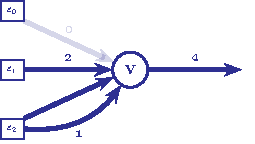
\includegraphics[width=\textwidth]{graphics/chapter2/flowConv2.pdf}
        \caption{}
        \label{fig: flowConv3}
    \end{subfigure}%
    \hfill
    \begin{subfigure}{0.4\textwidth}
        \centering
        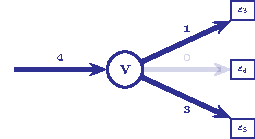
\includegraphics[width=\textwidth]{graphics/chapter2/flowConv3.pdf}
        \caption{}
        \label{fig: flowConv4}
    \end{subfigure}
    \vspace{0.2cm}
    \caption{The flow conservation constraint \ref{int_hyperflow_jakob} ensures steady-state mass conservation in the pathway. The induced hyperflow enforces that the number of copies of each vertex produced by the hyperedges equals the number of copies of the vertices used by the hyperedges. Case~\ref{fig: flowConv1} has no inflows or outflows ($v$ is neither a source vertex nor a target vertex), case~\ref{fig: flowConv2} satisfies Constraint \ref{int_hyperflow_jakob} but does not add anything physical to the pathway, case~\ref{fig: flowConv3} involves an outflow (which balances the number of copies of target vertex $v$ produced by the incident hyperedges), while case~\ref{fig: flowConv4} involves an inflow (where the number of copies of source vertex $v$ supplied is used by the out-going hyperedges).}
    \label{fig: flowConv}
\end{figure}

Since we are extending the existing integer hyperflow formulation defined earlier, the base ILP formulation for modeling flow conservation in pathways in reaction networks stated by Equation~\eqref{int_hyperflow_jakob} 
\[
\forall v\in V\colon \sum_{ e\in \overline{E} } s_{ve}^+ f_e - \sum_{ e\in \overline{E} } s_{ve}^- f_e = 0
\]

is inherited from that work. The working of Constraint~\eqref{int_hyperflow_jakob} is illustrated in the four example cases in Figure~\ref{fig: flowConv}. 

Any set of integer flow values on $E$ induces some overall reaction, which corresponds to flow values on $E^+ \cup E^-$ that make Equation~\eqref{int_hyperflow_jakob} hold.
However, the set of available source molecules is often constrained by practical considerations such as cost, ease of availability and purity.
Similarly, for the flow to be of practical utility, we could be interested in flows which maximize the outflow of a particular molecule, produce minimum side-products, and perhaps limit the use of particularly expensive reactions.
As explained while defining hyperflows, such conditions are modeled as constraints on the flow values $f_e$, in particular for $e$ in $E^+$ and $E^-$, but potentially also in $E$.
These constraints constitute a structural specification of the pathway searched for:
\begin{align}
    \text{Structural specification constraints on $f_e$ for } e \in \overline{E} \label{inflow_outflow_constraints}
\end{align}

To also incorporate thermodynamics into the modeling, we propose assigning a chemical potentials for each vertex $v$, $x^{G^0}_v$, under standard physical conditions,
which are calculated using a thermodynamic oracle described later in Chapter~\ref{ch:casestudy1}.
The differences in the chemical potentials of the target set and the source set in a reaction $e$, $x^{\Delta G}_e$, serve as the thermodynamic force driving the reaction, dictating the direction of flow of matter along that hyperedge.
In the linear regime, not far away from the equilibrium, the thermodynamic flows on a particular hyperedge is directly proportional to the thermodynamic force driving it.
The difference in chemical potential for a reaction can be manipulated by altering the concentrations of the molecules involved. 
We choose to represent the log concentration of a molecule $v$ by the variable $x_v^K$.
The nudged difference in chemical potentials for a reaction $e$ is represented as the variable, $x^{\Delta G}_e$ after taking into account the effect of the log concentration, $x_v^K$, of the molecules involved in the reaction $e$.
We would like to have an assignment of variables $x_v^K$ (within practical limits) such that the pathway consists of reactions with only negative differences in chemical potentials, of in other words, thermodynamically favorable reactions. The variables in the MILP formulation are listed in Table \ref{tab: MILPvariables}. 

\begin{table}[!t]
    \centering
    \begin{footnotesize}
    \begin{tabular}{clll}
        \\\toprule
        MILP variable & datatype & & description \\
        \midrule
        $f_e$ & integer & & flow variable for a hyperedge $e$ \\
        &&&  non-negative \\
        $x^{\Delta G}_e$ & float & & differences in chemical potential \\
        & & &  of in-vertices and out-vertices of a hyperedge $e$ \\
        & & & after accounting for their concentrations \\ 
        $x_v^K$ & float & & log concentration of a vertex $v$\\
        $t_v$ & integer & & topological ordering number \\
        &&& for vertex $v$, non-negative\\
        \midrule
        $x^{G^0}_v$ & float & & chemical potential of a vertex $v$ \\
        &&& under standard physical conditions \\
        & & & as assigned by the thermodynamic oracle \\
        $x^{\Delta G^0}_e$ & float & & differences in chemical potential \\
        &&& of in-vertices and out-vertices of a hyperedge $e$ \\
        & & & under standard physical conditions \\
        \bottomrule\\
    \end{tabular}
    \end{footnotesize}
    \caption{Variables used in the proposed constraint based formulation of pathways in a reaction network. These variables are used to formulate implication constraints in Section~\ref{milp_implication} which would be later linearized using additional auxiliary variables.}
    \label{tab: MILPvariables}
\end{table}

\begin{figure}[!h]
	\centering
	\vspace{1.5cm}
    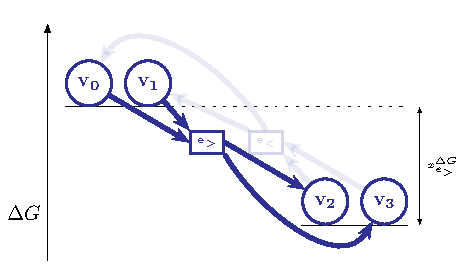
\includegraphics[width=0.75\textwidth]{graphics/chapter2/thermoConstraint.pdf}
    \vspace{0.5cm}
    \caption{Separate hyperedges have been added for the reaction $e_> : v_0 + v_1 \rightarrow v_2 + v_2$ and its reverse $e_< : v_2 + v_2 \rightarrow v_0 + v_1$. The difference in chemical potential for the hyperedge is calculated as $x_{e_>}^{\Delta G} = \Delta G(\text{RHS}) - \Delta G(\text{LHS}) = \left[\Delta G(v_2) + \Delta G(v_3)\right] - \left[\Delta G(v_0) + \Delta G(v_-)\right] = -x_{e_<}^{\Delta G}$. As a result of constraints~\ref{proposed_constraint2} and \ref{proposed_constraint3}, it is allowed to have a positive hyperflow only on the hyperedge corresponding to $e_>$. The hyperedge corresponding to $e_<$ might be assigned a hyperflow only when $x_{e_<}^{\Delta G} \leq 0$, by some possible assignment of the concentration variables $x_v^K$ of the vertices involved. Therefore, thermodynamic free energy differences dicatate the direction of mass flows in the network.}
    \label{fig: thermoConstraint}
\end{figure}

The flow $f_e$ through a hyperedge $e$ must be positive. 
\begin{equation}
    \forall e \in \overline{E}\colon  0 \leq f_e
    \label{proposed_constraint2}
\end{equation}
Since the reactions are reversible, separate hyperedges are added for the forward and backward directions.
Under specific physical conditions, thermodynamic forces dictates that either the forward or the backward direction of a reversible reaction is more likely. This is illustrated in Figure~\ref{fig: thermoConstraint}.
The direction of the flow is in the direction in which the difference in chemical potential for a hyperedge $e$, $x^{\Delta G}_e$, is negative.
The following implication-based constraint ensures that the pathway returned by the MILP solver consists of thermodynamically favorable reactions only.
\begin{equation}
    \forall e \in E\colon  f_e > 0 \implies x^{\Delta G}_e \leq 0 \label{proposed_constraint3}
\end{equation}
The difference in chemical potential, $x^{\Delta G}_e$ under arbitrary log concentration values, $x^K_v$ of the molecules participating in the reaction $e$ is calculated from the difference in chemical potential under standard conditions, $x^{G^0}_v$, by the following equations.
\begin{align}
    \forall e&\equiv (e^-, e^+) \in E\colon  \nonumber\\
    x^{\Delta G}_e &= \left(\sum_{v\in e^+} x^{G^0}_v - \sum_{v\in e^-} x^{G^0}_v\right) \nonumber\\
    &+ RT\cdot \left(\sum_{v\in e^+} x^K_v - \sum_{v\in e^-} x^K_v\right) \label{proposed_constraint4}
\end{align}
The molecules on the left side and right side of an elementary reaction belong to $e^-$ and $e^+$ respectively.
$R$ is the universal gas constant (in appropriate units) while $T$ is the absolute temperate of the system.
In a well-stirred system, $RT$ is a constant for the system.  
The log concentration of the molecules, $x_v^K$, is allowed to vary within a range $\left[x^K_v\right]_{\text{min}} \leq x_v^K \leq  \left[x^K_v\right]_{\text{max}}$,
set by practical and physical constraints detailed in Chapter \ref{ch:casestudy1}, to mimic the conditions inside a reactor.
\begin{equation}
    \left[x^K_v\right]_{\text{min}} \leq x^K_v \leq \left[x^K_v\right]_{\text{max}} \label{proposed_constraint8}
\end{equation}

\begin{figure}[!t]
    \centering
    \begin{subfigure}{\textwidth}
        \centering
        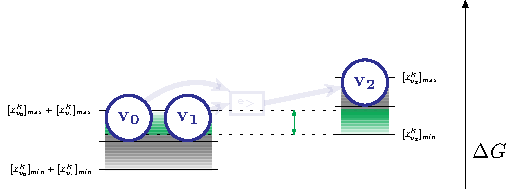
\includegraphics[width=0.75\textwidth]{graphics/chapter2/concTweak1.pdf}
        \vspace{0.4cm}
        \caption{with default values of $x_v^K$.}
        \label{fig: concTweak1}
    \end{subfigure}
    \\
    \vspace{0.8cm}
    \begin{subfigure}{\textwidth}
        \centering
        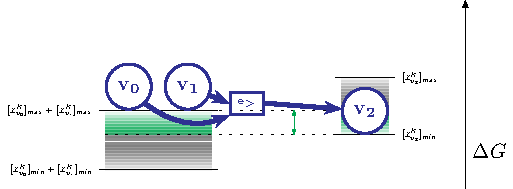
\includegraphics[width=0.75\textwidth]{graphics/chapter2/concTweak2.pdf}
        \vspace{0.4cm}
        \caption{after tweaking values of $x_v^K$}
        \label{fig: concTweak2}
    \end{subfigure}
    \vspace{0.5cm}
    \caption{Often hyperedges with assigned $x^{\Delta G^0}_e > 0$ (which are thermodynamically not feasible under standard physical conditions) can be made thermodynamically feasible by tweaking the concentration variables $x_v^K$ of the vertices involved. The hyperedge from Figure~\ref{fig: concTweak1} by raising the concentrations of vertices $v_0$ and $v_1$ and lowering the concentration of the vertex $v_2$ as shown in Figure~\ref{fig: concTweak2}.}
    \label{fig: concTweak}
\end{figure}

The control over the concentration of the molecules in the system is used in several practical scenarios to influence the equilibrium in the system.
Often, the concentration of certain molecules in the system are monitored and actively allowed to vary only within certain controlled ranges to facilitate (or inhibit) the formation of certain molecules in the system. 
The variation in the concentration of the molecules allows the model to be closer to reality, because stable molecules would have a higher concentration, while reactive intermediate molecules would be expected to have lower concentrations.
The variation in the concentration of the molecules can also make a reaction, that was thermodynamically infeasible under standard physical conditions, thermodynamically feasible under certain ranges of the concentration of the molecules involved as shown in Figure~\ref{fig: concTweak}. This then allows the corresponding hyperedge to have a non-negative flow, and be included in a pathway.

Note that the dependence of difference in the chemical potentials for a reaction $e$ on the concentrations of the molecules involved is not linear.
\begin{align*}
    x^{\Delta G}_e &= x^{\Delta G^0}_e + RT \ln\left(\frac{\prod_{v\in e^+} \text{conc}(v)}{\prod_{v\in e^-} \text{conc}(v)}\right) \\
    &= x^{\Delta G^0}_e + \frac{RT}{\ln 10}\left(\log\left(\prod_{v\in e^+} \text{conc}(v)\right)\right.\\
    & \text{\hspace{3cm}}- \left.\log\left(\prod_{v\in e^-} \text{conc}(v)\right)\right) \\
    &= x^{\Delta G^0}_e + \frac{RT}{\ln 10}\left(\sum_{v\in e^+} \log \text{conc}(v)\right.\\
    & \text{\hspace{3cm}}- \left.\sum_{v\in e^-} \log \text{conc}(v)\right)
\end{align*}
\begin{align*}
    & \text{ where, }\\
    x^{\Delta G^0}_e &= \sum_{v\in e^+} x^{G^0}_v - \sum_{v\in e^-} x^{G^0}_v
\end{align*}
However, it can be represented as a linear expression, if one chooses to represent the log concentrations of the corresponding molecule $v$, $\log_{10} \text{conc}(v)$, as a variable $x_v^K$, in the linear program. 


\subsection{Objective Function}

Formulating the search for pathways in reaction networks as an MILP problem,
allows us to add an implication constraint to rule out pathways containing one or more individual reactions not favored by thermodynamics.
However, it also enables us to exploit another feature of MILPs,
namely the objective function to quantify how likely is the entire pathway to occur.

We would like to formulate the search for pathways as an optimization problem aimed at maximizing the outflow of the target molecule(s).
To maximize the intended objective, we attempt to maximize the net thermodynamic force driving the flow.
Considering the net thermodynamic forces driving the flow to be the sum of the thermodynamic driving force for each individual reaction in the pathway,
we choose as objective function the minimization of the cumulative sum of the difference in chemical potentials for each constituent reaction with a non-zero flow. 
\begin{equation}
    \max \left(- \sum_{e\colon f_e > 0} x^{\Delta G}_e \right)
    \label{objective function}
\end{equation}
This choice of the objective function~\eqref{objective function} is a heuristic which fits  well with the cost of perturbing the system so that queried flow is effected with all reactions being thermodynamically driven in the required direction. 
Objective function~\eqref{objective function} can be related to optimal control principles and considered as the minimum work required to be done to enforce the hyperflow $f: \{e | f_e > 0\}$. Once the system is in equilibrium, it has to be slightly perturbed out of that equilibrium to sustain the hyperflow $f$.
The minimal work required to be performed to achieve the required perturbation should satisfy
\begin{equation*}
	\langle W_{\text{min}} \rangle \geq \sum_{e\colon f_e > 0} x^{\Delta G}_e
\end{equation*}
This is similar to the Crooks fluctuation theorem~\cite{crooks,crooks2} and its implication, the Jarzynski inequality~\cite{jarzynski,jarzynski2,jarzynski3}.\footnote{Equation (2) in~\cite{jarzynski} and equations (3.2) and (3.4a) in~\cite{jarzynski2} have a similar form involving the free energy on the right-hand side.}
All in all, ranking pathways by the objective function~\eqref{objective function} corresponds closely to selecting the pathway that requires the least thermodynamic work to sustain the outflow of the queried target molecule. Maximizing objective function~\eqref{objective function} becomes equivalent to minimizing the work done to perturb the system from equilibrium to achieve the desired hyperflow. 

The motivation behind choosing this particular objective function can also be argued for from the perspective of maximizing the probability of the pathway.
We interpret the free energy difference to be the measure of the probability of the reaction as
\begin{equation}
    p(e) \sim \exp\left(-x^{\Delta G}_e\right)
    \label{prob_transition}
\end{equation}
This probability for a reaction $e$ can also be argued for using the principle of local detailed balance between the rates of the reaction and its reverse where \footnote{Markovian trajectories might be coarse-grained into pathways (sets of reactions with positive hyperflow) under dilute limit, Markovian kinetics, and weak coupling between reactions.}
\begin{equation*}
    \frac{k_+(e)}{k_-(e)} = \exp\left(-\frac{x^{\Delta G}_e}{k_B T}\right)
\end{equation*}
For a Markovian process describing the sequence of reaction events along the pathway, the probability of observing the specific trajectory over time satisfies
\begin{align*}
    p\left(\bigwedge_{e\colon f_e > 0} e\right) &= \prod_{e: f_e > 0} p(e) \\
    &\sim \prod_{e\colon f_e > 0} \exp\left(-x^{\Delta G}_e\right) \\
    &= \exp\left(- \sum_{e: f_e > 0} x^{\Delta G}_e\right)
\end{align*}
Thus, for paths biased in the direction of the pathway (compared to the reverse direction), $-x^{\Delta G}_e$ accumulates additively in the exponent for the probablity.
Since, $\forall (x, y)\colon  x\leq y \iff \exp(x) \leq \exp(y)$,
maximizing the probability of the pathway is equivalent to maximizing the objective function~\eqref{objective function}.
\begin{equation*}
    \text{max} \log \left[p\left(\bigwedge_{e\colon f_e > 0} e\right)\right] \equiv \text{max} - \sum_{e: f_e > 0} x^{\Delta G}_e
    \label{log_prob}
\end{equation*}
Therefore, in the low-noise, steady-state, weak-coupling limit, maximizing the log-probability of sustaining a pathway with the hyperedges with assigned positive hyperflows decomposes approximately as maximizing a sum of negative of reaction-wise free-energy differences. The RHS of this expression~\eqref{log_prob} is the negation of the action associated with producing the desired hyperflow which is correspondingly minimized. The additivity of the objective function can be justified by the convexity of the rate function for perturbations in chemical reaction networks given by the Wentzell-Freidlin theory.~\cite{convex_rate_law}

A third way to motivate objective function~\eqref{objective function} is to use the driving force for reactions. For a reaction $e$, the thermodynamic driving force is the negative of the Gibbs free energy difference~\cite{driving_force} or $-x^{\Delta G}_e$ (which is closely related to the affinity of reactions~\cite{affinity} and positive for spontaneous reactions). The net driving force along a hyperflow would be $- \sum_{e\colon f_e > 0} x^{\Delta G}_e$ (as all hyperflows are positive, the net force adds up). Therefore, the objective corresponds to selecting pathways that are most strongly thermodynamically driven, hence most robust to perturbations.  

All in all, the objective is defensible as a heuristic, and can be motivated by a physical interpretation—but only under fairly explicit assumptions, rather than a strict consequence of the laws of thermodynamics. It should be seen more as a ranking functional, rather than a dynamical law.

\section{Implementation}
\label{milp_implement}

The objective function is a conditional sum for a set of MILP variables.
The value of the variable $x^{\Delta G}_e$ contributes to the objective function only if the corresponding hyperedge is used in the pathway.
It needs to be converted into a simple linear sum of a set of MILP variables before the MILP solver can evaluate it.  
Additionally, some constraints such as \eqref{proposed_constraint3} and \eqref{prevent_back_edges} in the mathematical formulation of the problem have been specified as implications. 
Also they need to be linearized before fed into the MILP solver.
This section describes these implementation details for the formulated MILP model in the previous section.

\subsection{Implementing the Objective function}

The objective function minimizes the cumulative sum of the differences in chemical potentials along the pathway,
$\min\left(\sum_{e\colon f_e > 0} x^{\Delta G}_e \right)$,
rather than the simple sum of differences in chemical potentials.
For all reactions $e$, $\min\left(\sum_{e \in E} x^{\Delta G}_e \right)$, in the reaction network. 
For each hyperedge $e$, a binary variable $z_e \in \{0, 1\}$ is introduced,
indicating whether that hyperedge is used in the pathway, by the following constraints
\begin{align}
    z_e = 0 &\iff f_e = 0 \label{biimp3} \\
    z_e = 1 &\iff f_e > 0 \label{biimp4}
\end{align}
We define an additional variable $\overline{x}^{\Delta G}_e$ for each hyperedge.

The assignment of the variables $\overline{x}^{\Delta G}_e$ is done by the following constraints
\begin{align}
    \overline{x}^{\Delta G}_e = 0 &\iff z_e = 0 \label{biimp1} \\
    \overline{x}^{\Delta G}_e = x^{\Delta G}_e &\iff z_e = 1 \label{biimp2}
\end{align}
The objective function is defined as the sum of these $|E|$ variables for all hyperedges in the hypergraph;
$\min\left(\sum_{e \in E} \overline{x}^{\Delta G}_e \right)$.
Hyperedges that are not utilized by the pathway have $\overline{x}^{\Delta G}_e = 0$ and would not contribute to the value of the objective function, implementing the objective function as a linear expression.


\subsection{Linearizing the Constraints}

The bi-implication constraints, Equations~\eqref{biimp3} and \eqref{biimp4}, associating the boolean variable $z_e$ to the edges $e$ is implemented using the big-M method ~\cite{bigM},
where $M > 0$ is a large positive integer constant% dont remove comment, escapes newline
\footnote{The constant $M$ has to be larger than the possible values of the variables in the MILP formulation which include the flows $f_e$ for the hyperedges and the chemical potentials $x^{G^0}_v$ for the vertices (in atomic units). In our present implementation $M = 100$ suffices.}
\begin{align}
    \forall e \in E\colon & \nonumber \\
    z_e &\leq f_e \label{linear_constraint6}\\
    M\cdot z_e &\geq f_e \label{linear_constraint7}
\end{align}
The expansion of how the added linear constraints in Equations~\eqref{linear_constraint6} and \eqref{linear_constraint7}
lead to assignment of $z_e$ satisfying the implication constraints in Equations~\eqref{biimp3} and \eqref{biimp4}
is shown in Table~\ref{tab: truth_table_constraint1}.
\begin{table}[!t]
    \centering
    \begin{footnotesize}
    \begin{tabular}{cccc}
        \\\toprule
        case of $f_e$ & \eqref{linear_constraint6} & \eqref{linear_constraint7} & implication for $z_e$ \\
        \midrule
        $f_e = 0$ & $z_e \leq 0$ & $M\cdot z_e \geq 0$ & $z_e = 0$ \\
        $f_e = k > 0$ & $z_e \leq k$ & $M\cdot z_e \geq k$ & $z_e = 1$ \\
        \bottomrule\\
    \end{tabular}
    \end{footnotesize}
    \caption{The linear constraints in Equations \eqref{linear_constraint6} and \eqref{linear_constraint7}
    are equivalent to the bi-implication constraints in Equations \eqref{biimp3} and \eqref{biimp4}.}
    \label{tab: truth_table_constraint1}
\end{table}

The implication constraint in Equation~\eqref{proposed_constraint3} determines if an hyperedge can be used in the flow depending on the differences in the chemical potentials for the hyperedges $x^{\Delta G}_e$.
This is linearized as
\begin{align}
    \forall e \in E\colon & \nonumber \\
    x^{\Delta G}_e + M\cdot (z_e - 1) &\leq 0 \label{linear_constraint1}
\end{align}
The equivalence of the added linear constraints in Equation~\eqref{linear_constraint1} to the implication constraint in Equation~\eqref{proposed_constraint3} is shown in Table~\ref{tab: truth_table_constraint2}.
\begin{table*}[!t]
    \centering
    \begin{footnotesize}
    \begin{tabular}{ccccc}
        \\\toprule
        case of $f_{e}$ & implication for $z_{e}$ & case of $x^{\Delta G}_e$ & \eqref{proposed_constraint3} satisfied? & \eqref{linear_constraint1} satisfied? \\
        \midrule
        $f_{e} = 0$ & $z_{e} = 0$ & $x^{\Delta G}_e > 0$ & True & True \\
        $f_{e} = 0$ & $z_{e} = 0$ & $x^{\Delta G}_e \leq 0$ & True & True \\
        $f_{e} > 0$ & $z_{e} = 1$ & $x^{\Delta G}_e > 0$ & False & False \\
        $f_{e} > 0$ & $z_{e} = 1$ & $x^{\Delta G}_e \leq 0$ & True & True \\
        \bottomrule\\
    \end{tabular}
    \end{footnotesize}
    \caption{The linear constraint in Equation~\eqref{linear_constraint1} is equivalent to the implication constraint in Equation~\eqref{proposed_constraint3}.}
    \label{tab: truth_table_constraint2}
\end{table*}

The bi-implication constraints in Equations~\eqref{biimp1} and \eqref{biimp2} assigns the variable $\overline{x}^{\Delta G}_e$ with the differences in the chemical potentials for the hyperedges for the evaluation of the objective function.
By utilizing the variables $z_e$, we implement the constraints as
\begin{align}
    \forall e \in E\colon & \nonumber \\
    x^{\Delta G}_e - \overline{x}^{\Delta G}_e &\leq M(1 - z_e) \label{linear_constraint2} \\
    x^{\Delta G}_e - \overline{x}^{\Delta G}_e &\geq -M(1 - z_e) \label{linear_constraint3} \\
    \overline{x}^{\Delta G}_e &\leq M\cdot z_e \label{linear_constraint4} \\
    \overline{x}^{\Delta G}_e &\geq -M\cdot z_e \label{linear_constraint5}
\end{align}
The expansion of how the added linear constraints in Equations~\eqref{linear_constraint2}, \eqref{linear_constraint3}, \eqref{linear_constraint4}, and \eqref{linear_constraint5} lead to desired assignment of $\overline{x}^{\Delta G}_e$ satisfying the implication constraints in Equations~\eqref{biimp1} and \eqref{biimp2} is shown in Table~\ref{tab: truth_table_constraint3}.

\begin{table*}[!t]
    \centering
    \begin{footnotesize}
    \begin{tabular}{@{}c@{\qquad}c*{4}{@{\qquad}c}l@{\qquad}c@{}}
        \toprule
        &&\multicolumn{4}{c}{Constraint on $\overline{x}^{\Delta G}_e$ by}\\
        \cmidrule{3-6}
        Case of $z_{e}$ & Case of $x^{\Delta G}_e$ &
            \eqref{linear_constraint2} & \eqref{linear_constraint3} & \eqref{linear_constraint4} & \eqref{linear_constraint5} &
        & Implication for $\overline{x}^{\Delta G}_e$ \\
        \midrule
        $z_{e} = 0$ & $x^{\Delta G}_e > 0$ & & & $\leq 0$ & $\geq 0$ && $=0$ \\
        $z_{e} = 0$ & $x^{\Delta G}_e \leq 0$ & & & $\leq 0$ & $\geq 0$ && $=0$ \\
        $z_{e} = 1$ & $x^{\Delta G}_e > 0$ &
            \multicolumn{6}{c}{
                \raisebox{0.5ex}{\rule{8.5em}{0.4pt}}
                \enspace Cannot happen \enspace
                \raisebox{0.5ex}{\rule{8.5em}{0.4pt}}
                } \\
        $z_{e} = 1$ & $x^{\Delta G}_e \leq 0$ & $\geq x^{\Delta G}_e$ & $\leq x^{\Delta G}_e$ & & && $= x^{\Delta G}_e$ \\
        \bottomrule
    \end{tabular}
    \end{footnotesize}
    \caption{The linear constraints of Equation~\eqref{linear_constraint2}, \eqref{linear_constraint3}, \eqref{linear_constraint4}, and \eqref{linear_constraint5}
    assign $\overline{x}^{\Delta G}_e$ according to the bi-implication constraints in Equations~\eqref{biimp1} and \eqref{biimp2}.
    Note that the third case cannot happen due to Equation~\eqref{proposed_constraint3},
    because $x^{\Delta G}_e > 0 \implies f_e = 0 \implies z_e = 0$.}
    \label{tab: truth_table_constraint3}
\end{table*}


\subsection{Implemented Model}\label{implemented model}

\begin{table*}[!b]
    \centering
    \begin{footnotesize}
    \begin{tabular}{clll}
        \toprule
        Constant & datatype & & description \\
        \midrule
        $M$ & integer & & a big integer used for \\
        &&& linearizing the constraints \\
        & & & (type promoted to float, if required) \\
        $x^{G^0}_v$ & float & & chemical potential of a vertex $v$ \\
        &&& under standard physical conditions \\
        & & & as assigned by the thermodynamic oracle \\
        $x^{\Delta G^0}_e$ & float & & differences in chemical potential \\
        &&& of in-vertices and out-vertices of a hyperedge $e$ \\
        & & & under standard physical conditions \\
        \bottomrule
    \end{tabular}
    \end{footnotesize}
    \caption{Constants in the proposed MILP formulation.
    The constants $M$ and $x^{G^0}_v$ are provided as input,
    while the constants $x^{\Delta G^0}_e$ are calculated based on the given $x^{G^0}_v$.
    }
    \label{tab: MILP constants}
\end{table*}%


For an overview, we here list the entire set of variables of the model in Table~\ref{tab: MILP variables} and the constants used in the model in Table~\ref{tab: MILP constants}. We also summarize the mixed integer linear program developed in the earlier sections.
This model is what is given to the MILP solver.

\begin{table*}[!t]
    \centering
    \begin{footnotesize}
    \begin{tabular}{clll}
        \toprule
        MILP variable & datatype & & description \\
        \midrule
        $f_e$ & integer & & flow variable for a hyperedge $e$ \\
        &&& non-negative \\
        $z_e$ & boolean & & indicator variable for a hyperedge $e$ \\
        & & & denoting if it is used in the flow \\
        $x^{\Delta G}_e$ & float & & differences in chemical potential \\
        & & &  of in-vertices and out-vertices of a hyperedge $e$ \\
        & & & after accounting for their concentrations \\ 
        $\overline{x}^{\Delta G}_e$ & float & & copy of $x^{\Delta G}_e$ used in the (linearized) objective function \\
        $x_v^K$ & float & & log concentration of a vertex $v$\\
        $t_v$ & integer & & topological ordering number \\
        &&& for vertex $v$, non-negative\\
        \bottomrule
    \end{tabular}
    \end{footnotesize}
    \caption{Variables in the proposed MILP formulation.}
    \label{tab: MILP variables}
\end{table*}%

The formulated MILP is:
\begin{align}
    & \min\left(\sum_{e \in E} \overline{x}^{\Delta G}_e \right) \label{obj_func_impl} \\    
    \forall v\in V\colon  & \sum_{ e\in \overline{E} } s_{ve}^+ f_e - \sum_{ e\in \overline{E} } s_{ve}^- f_e = 0 \tag{\ref{int_hyperflow_jakob}}
\end{align}
\begin{align}
    \text{Structural speci}&\text{fication constraints on $f_e$ for } e \in \overline{E} \tag{\ref{inflow_outflow_constraints}}\\
    \forall e&\equiv (e^-, e^+) \in E\colon \nonumber\\
    0 &\leq f_e  \tag{\ref{proposed_constraint2}} \\
    x^{\Delta G}_e &= \left(\sum_{v\in e^+} x^{G^0}_v - \sum_{v\in e^-} x^{G^0}_v\right) \nonumber\\
    & \hspace{0.5cm}+ RT\cdot \left(\sum_{v\in e^+} x^K_v - \sum_{v\in e^-} x^K_v\right) \tag{\ref{proposed_constraint4}} \\    
    0 &\geq x^{\Delta G}_e + M\cdot (z_e - 1) \tag{\ref{linear_constraint1}} \\
    M(1 - z_e) &\geq x^{\Delta G}_e - \overline{x}^{\Delta G}_e  \tag{\ref{linear_constraint2}} \\
    -M(1 - z_e) &\leq x^{\Delta G}_e - \overline{x}^{\Delta G}_e \tag{\ref{linear_constraint3}} \\
    M\cdot z_e &\geq \overline{x}^{\Delta G}_e \tag{\ref{linear_constraint4}} \\
    -M\cdot z_e &\leq \overline{x}^{\Delta G}_e \tag{\ref{linear_constraint5}} \\
    \forall v \in V\colon  & \nonumber\\
    0 &\leq t_v \leq |V| \tag{\ref{linear_constraint7}} \\
    \left[x^K_v\right]_{\text{min}} &\leq x^K_v \leq \left[x^K_v\right]_{\text{max}} \tag{\ref{proposed_constraint8}}\\\nonumber
\end{align}

The computational complexity of finding MILP solutions is in general NP-hard~\cite{Karp:72},
and even the restricted case of finding chemical pathways remains so~\cite{integer_hyperflow_np_hard}.
Despite this worst case complexity, modern MILP solvers efficiently handle most practically relevant instances in reasonable time.
From a thermodynamic perspective, it is often valuable to explore \emph{multiple} optimal or near-optimal solutions---however, MILP solvers generally only provide a single optimal solution.
Some solvers, e.g., IBM ILOG CPLEX, do provide a so-called solution pool facility for enumerating multiple solutions,
but there is little user-control for how it is populated, and in particular how solutions are compared for equality.

The thermodynamics module described in this contribution is implemented as an extension of the larger software package M{\O}D~\cite{jakob_software}, available at \url{http://mod.imada.sdu.dk/}.
The package offers the option of using multiple MILP solvers, currently IBM ILOG CPLEX, Gurobi, and Coin-OR CBC.
For the results presented here we have used Coin-OR CBC~\cite{cbc,cbc2}.
M{\O}D implements a MILP enumeration algorithm on top of the solver in use,
where one can specify a set of integer or binary variables to enumerate over.
This enumeration in M{\O}D proceeds as tree search algorithm over the domains of this set of variables,
with calls to the MILP solver for evaluating feasibility obtaining optimal solutions of subproblems~\cite{jakob_integer_hyperflows}.

In the MILP model presented here, there are variables with a continuous domain representing the concentrations and chemical potentials of the molecules.
We do not consider minor changes in these variables to represent a new solution, as long as the underlying flow is unchanged.
Hence, we carry out the enumeration over the variables $f_e,\forall e\in E$.
The resulting output is a list of different integral flows,
listed in the order of increasing value of the objective function \eqref{obj_func_impl}.

%************************************************
\section{Contextualizing this Method}
\label{discussions_method} %
%************************************************

In this section, we give a detailed comparison of our methods with some existing frameworks.
One of the closest is \emph{thermodynamics-based metabolic flux analysis} (TMFA) \cite{hatz_thermo_flow} which also utilizes mixed integer linear constraints.
Despite similarities in parts of the thermodynamic modeling, the problem solved is different, with some of the key differences being:
\begin{itemize}
    \item TMFA generates \emph{flux distributions} not containing thermodynamically infeasible reactions, while our method searches for \emph{explicitly specified pathways} mot containing thermodynamically unfavorable reactions. The flux vector generated by TMFA is real-valued as opposed to integer values for the flows in the pathways determined by our method. In many settings, the concept of a pathway involves an integer number of molecules participating in each reaction of the pathway, which aligns well with integer flows.
    \item TMFA uses a curated dataset of metabolites with chemical potentials determined by group contribution methods. In our case a semi-empirical method (GFN2-xTB) is used to assign chemical potentials to the molecules in the reaction network. However, it can be substituted by any suitable `oracle' that maps a molecule to its Gibbs free energy of the user choice. This provides flexibility and a wider applicability to this method.
    \item  We allow for a ranking of the enumerated results based on thermodynamics-based metrics. In terms of the linear program modeling, restricting the flow variables to integers allows us to enumerate solutions over the integral variables (i.e., to generate not just a single solution, but many).
    Additionally, we can enforce a partial ordering of the vertices in the returned integer hyperflow solutions, in order to guarantee their realizability as synthesis plans.
\end{itemize}

We now turn to a comparison with some of the other existing frameworks.
Formulating the problem as an MILP allows us to leverage the many algorithmic advances made in the field of MILP solvers.
This may be one reason why we are able to analyze larger reaction networks than those analyzed in \cite{miangolarra_non_ideal_CRN, seifert_thermodynamics_CRN_JCP, nicolis_thermodynamics_CRN} involving a smaller number of distinct molecules.
A further difference to these works is that they utilize kinetic rate equations derived from the law of mass action (reactions under kinetic control),
while our focus is on the differences in chemical potentials of the molecules in the reaction network near equilibrium (reactions under thermodynamics control).

Weighted directed graphs are utilized in \cite{synthesis_planning_CRN_thermodynamics} to model the thermodynamic phase space of a reaction network.
However, instead of a constant positive edge weight derived from the Gibbs free energy of the reaction,
we utilize the free energies themselves to allow for an analysis more directly based on thermodynamics.
Several other cheminformatics tools and automated protocols for computationally exploring reaction networks utilize reactive molecular dynamics simulations \cite{CRN_MD_tool1, CRN_MD_tool2, CRN_MD_tool3} or chemical heuristics \cite{CRN_kin_tool1, CRN_kin_tool2, CRN_kin_tool3, pickaxe_CRN_analyzer}.
However, to the best of our knowledge, there does not exist any computational framework for explicitly specifying and searching for pathways in reaction networks while simultaneously incorporating thermodynamic constraints in the present form. 


%************************************************
\chapter{A Case Study: Foramide Chemistry}
\label{ch:casestudy1} %
%************************************************

{\sffamily\slshape The text in this chapter is identical to Section 4 of the published version of the preprint at \href{https://arxiv.org/abs/2411.15900}{arXiv:2411.15900}.\\}

In this chapter, we demonstrate the methods from Chapter~\ref{ch:thermodynamic_model} on a reaction network involving hydrogen cyanide, formamidic acid, and formamide in aqueous solution which has been studied in \cite{implemented_CRN}.

\section{Network Generation}

The reaction network was generated using M{\O}D by the expansion of the molecular space with the input molecules HCN, NH$_3$, and H$_2$O, by the recursive application of the graph transformation rules listed in Figure~\ref{fig: graphTransformationRules}.
The individual molecules in the generated network, such as HCN, NH$_3$, H$_2$O, formamide and so on, are represented as undirected labeled graphs.
\footnote{The atoms represented as vertices, labeled by the symbol of the element it represents, such as $C$ for a carbon atom, $H$ for a hydrogen atom, $N$ for a nitrogen atom, $O$ for an oxygen atom and so on. The bonds are represented as edges, labeled by bond types such as a single, double, triple or aromatic bond. The default bondtype is single.}
Stereo-information is not represented. Therefore, both the stereoisomers of the molecule shown in Figure~\ref{fig: molGraphs} are represented by the same graph. Hence, they cannot be distinguished in our modeling despite them being two different chemical entities.
Molecular graphs also constitute the vertices of the hypergraph representing the reaction network. 

\begin{figure}[b]
	\centering
    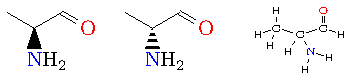
\includegraphics[scale=1.5]{graphics/chapter3/molGraphs.pdf}
    \vspace{0.2cm}
    \caption{Two stereoisomers of a molecule (left) and the corresponding molecular graph (right).}
    \label{fig: molGraphs}
\end{figure}

\begin{figure}[!t]
    \centering
    \begin{subfigure}{\textwidth}
        \centering
        \includegraphics[scale=1.5]{graphics/chapter3/rule0.pdf}
        \vspace{0.2cm}
        \caption{Addition to a cyanide: in this rule \texttt{x} $\in$ \{N, O\}, representing the addition of an amide nitrogen or hydroxyl oxygen to the nitrile bond respectively.}
        \label{fig:rule0}
    \end{subfigure}
    \\
    \vspace{0.5cm}
    \begin{subfigure}{\textwidth}
        \centering
        \includegraphics[scale=1.5]{graphics/chapter3/rule1.pdf}
        \vspace{0.2cm}
        \caption{Addition to an imine or carbonyl: in this rule \texttt{x}, \texttt{y} $\in$ \{N, O\}, representing the addition of an amide nitrogen or hydroxyl oxygen to an amide or hydroxyl bond respectively. This single rule encapsulates $2^2 = 4$ individual rules depending on the instantiation of \texttt{x} and \texttt{y}.}
        \label{fig:rule1}
    \end{subfigure}
    \\
    \vspace{0.5cm}
    \begin{subfigure}{\textwidth}
        \centering
        \includegraphics[scale=1.5]{graphics/chapter3/rule2.pdf}
        \vspace{0.2cm}
        \caption{1,3 hydrogen shift: in this rule \texttt{x}, \texttt{y} $\in$ \{C, N, O\}, representing the shift of a double bond as in tautomerism. When \texttt{x}$\equiv$O and \texttt{y}$\equiv$O it is keto-enol tautomerism, \texttt{x}$\equiv$N and \texttt{y}$\equiv$N is imine-enamine tautomerism, \texttt{x}$\equiv$N and \texttt{y}$\equiv$O is amine-iminol tautomerism and \texttt{x}$\equiv$C and \texttt{y}$\equiv$C is an allylic shift of the double bond. This single rule encapsulates $3\times 3 = 9$ individual rules depending on the instantiation of \texttt{x} and \texttt{y}.}
        \label{fig:rule2}
    \end{subfigure}%
    \\
    \vspace{0.5cm}
    \begin{subfigure}{\textwidth}
        \centering
        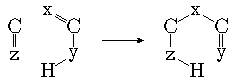
\includegraphics[scale=1.5]{graphics/chapter3/rule3.pdf}
        \vspace{0.2cm}
        \caption{Condensation: in this rule \texttt{x} $\in$ \{C, N, O\}, \texttt{y},\texttt{z} $\in$ \{N, O\} representation of the addition of a double bond (of an enol, enamine) to a imine or a carbonyl group. This single rule encapsulates $3\times 2\times 2 = 12$ individual rules depending on the instantiation of \texttt{x}, \texttt{y} and \texttt{z}.}
        \label{fig:rule3}
    \end{subfigure}%
    \vspace{0.5cm}
    \caption{The graph transformation rules used to expand the molecular space and generate the network.}
    \label{fig: graphTransformationRules}
\end{figure}

\begin{figure}[!h]
	\centering
	\vspace{0.5cm}
    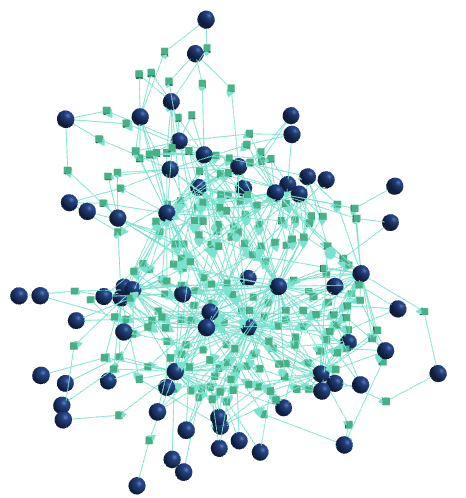
\includegraphics[width=0.8\textwidth]{graphics/chapter3/reactionNetworkChapter3.png}
    \vspace{0.5cm}
    \caption{An abstract representation of the generated reaction network with $67$ vertices (blue circles) and $202$ hyperedges (green squares), on which the working of the method proposed in Chapter~\ref{ch:thermodynamic_model} was demonstrated.}
    \label{fig: hypergraphRNChapter3}
\end{figure}

The graph transformation rules in Figure~\ref{fig: graphTransformationRules} represent classes of reactions, i.e. reaction templates. The left hand side of the rules is a subgraph, which may be substituted by the subgraph on the right hand side, when a match has been found in a molecular graphs present in the reaction network. This executes a reaction, thereby expanding the molecular space. Following the previous study of the network \cite{implemented_CRN}, the expansion was constrained to only generate molecules with a maximum of three carbon, three nitrogen, and three oxygen atoms. Moreover, only stable molecules ($x_v^{G^0} \leq 0$) were kept. 
The generated reaction network consists of $67$ vertices and $202$ hyperedges, and is shown in Figure~\ref{fig: hypergraphRNChapter3} for completeness.
A list of all molecules and transitions in the reaction network can be found in the associated GitHub repository \cite{data_repository}.

\section{Thermodynamic Oracle}
\label{sec:oracle} %

\begin{figure}[!t]
	\centering
    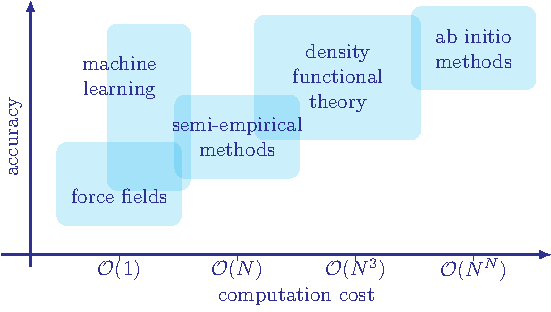
\includegraphics[width=0.8\textwidth]{graphics/chapter3/compCostCC.pdf}
    \vspace{0.5cm}
    \caption{A comparison of the computational costs of the available methods often used to assign free energies to molecules along with their accuracy. The rough ranges for the data used to draw the figure was collated from~\cite{ccCost}.}
    \label{fig: compChemCost}
\end{figure}

Given a reaction network, we assign chemical potentials to the molecules using what we had earlier referred to as a `thermodynamic oracle' in Chapter~\ref{ch:thermodynamic_model}. Utilizing quantum mechanical methods based on density functional theory (DFT) as this `thermodynamic oracle' quickly becomes impractical as the number of electrons in the molecule (denoted by $N$) increases, as indicated by the comparative computational costs of the different available methods as shown in Figure~\ref{fig: compChemCost}.
Calculating the electron density in a molecule using DFT is an iterative process. Each step invokes gradient descent, which scales beyond $\mathcal{O}(N^3)$ for classical DFT based methods for a single-point calculation because it involves matrix inversions. After the electron density for the molecule has been optimized, it can then be used to calculate the electronic contribution to the energy of a molecule.
Machine learnt relations for potential assignment exist, some require optimized atomic coordinates to determine potentials~\cite{NN_molecule_energies}, while others just utilize the connectivity of the molecular graph~\cite{ml_energy,ml_energy1,ml_energy2,ml_energy3} or even a string representation of it~\cite{ml-energy4}. However, these machine learnt relations from a dataset might not be well generalizable; they could perform poorly when a molecule sufficiently different, from those in the dataset trained on, is encountered~\cite{ml_energy5,ml_energy6,ml_energy7}. Ideally, kinetic rate parameters would have to be incorporated into the search for pathways in a reaction network as integer flows, because they dictate which reactions actually occur in the system and how fast. However, calculating activation free energies using DFT-based quantum mechanical methods to determine these kinetic parameters would demand even further time and computational resources.

\begin{figure}[!t]
	\centering
	\vspace{0.5cm}
    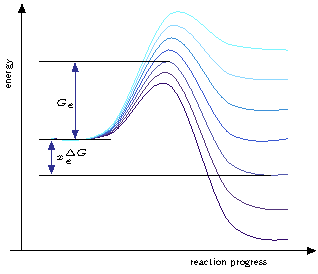
\includegraphics[width=0.8\textwidth]{graphics/chapter3/epsPrinciple.pdf}
    \vspace{0.5cm}
    \caption{In a group of not too diverse reactions, the energy barrier of a reaction can be considered to be dependent on the free energy change of the reaction by some function: $G_e = f\left(x_e^{\Delta G}\right)$. This holds because the reaction trajectories do not tend to cross each other when plotted normalized by the energy of the reactants.}
    \label{fig: epsPrinciple}
\end{figure}

As an alternative, we in this work adopt a compromise oracle based on equilibrium thermodynamics. This approximation has some theoretical basis behind it with the Evans– Polanyi–Semenov principle~\cite{epsPrinciple}, which states that within a class of reactions, the thermodynamics of the reaction acts as a proxy for the kinetics of the reaction, as shown in Figure~\ref{fig: epsPrinciple}. It allows us to substitute the energy barrier for a reaction with the free energy difference for a reaction resulting in the relation in Equation~\eqref{prob_transition}. Specifically, to balance accuracy, efficiency, generalizability, and running time, we employ a semi-empirical method, GFN2-xTB~\cite{grimme_xtb}, for potential assignment. While this method compromises on accuracy compared to DFT, the errors are acceptable for demonstrating the utility of the mathematical model on an example reaction network.
We detail the thermodynamic oracle we use to assign the chemical potentials to the molecules, $x_v^{G^0}$, in the reaction network in the following section.
An advantage of this modular approach is that it provides the reader the freedom to substitute the proposed thermodynamic oracle with another tool, for example pre-trained neural networks, mapping a molecule to its chemical potential (or even the reactions to their kinetics parameters) depending on the desired accuracies and available computational resources.

\section{On assigning the Chemical Potentials}\label{first appendix}

One of the main enhancements to the thermodynamic modeling of reaction networks in this work is a more robust, transparent and generic method of assigning the chemical potentials under standard physical conditions for molecules, $x^{G^0}_v$,
compared to relying on thermodynamic databases such as (\url{https://pytfa.readthedocs.io/en/latest/thermoDB.html})
 using the group contribution method, to infer the free energy change for reactions, $x^{G^0}_e$, 
as done in~\cite{hatz_therm_python}.
Using quantum chemical methods to assign these chemical potentials quickly becomes computationally resource-intensive because the time complexity scales as $\mathcal{O}(N^3)$. The density-functional theory (DFT) calculations involve diagonalization of the $N\times N$ Hamiltonian matrix. 
The memory requirement scales as $\mathcal{O}(N^2)$ because of the number of two-electron integrals contributing to the energy of the system. Moreover, it is an iterative process which is repeated until an acceptable convergence criteria is reached.

\begin{figure}[!t]
    \centering
    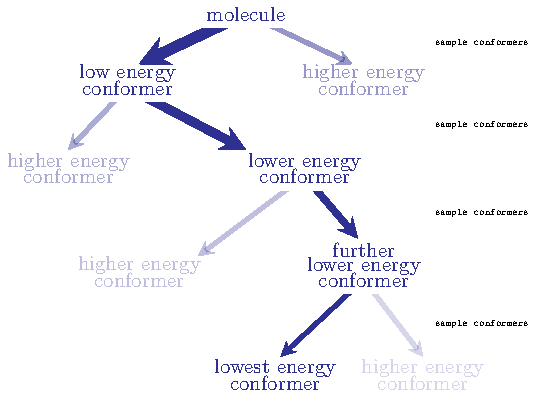
\includegraphics[width=0.9\textwidth]{graphics/chapter3/sampleConformer.pdf}
    \vspace{0.5cm}
    \caption{OpenBabel's \texttt{WeightetedRotorSearch()} iteratively samples conformers to reach towards the lowest energy conformer of the molecule. It randomly chooses from the allowed torsion angles, and reweights the choice based on the energy of the last generated lowest energy conformer. Progressively, the generated conformer has increasingly lower energy.}
    \label{fig: sampleConformer}
\end{figure}

Efficient software design necessitates striking a balance among the components in this work: expanding the molecular space, assigning chemical potentials to the molecules in the space and solving the formulated MILP for queried pathways in the network.   
If DFT calculations are employed, the calculation of chemical potentials required a significantly longer time compared to the remaining two components.
Alternative semi-empirical methods offered a faster yet reasonable accurate way to assign chemical potentials to molecules.
Therefore, we utilized xTB~\cite{grimme_xtb} to estimate the chemical potentials for the molecules in the expanded reaction network.
In the rest of this Section, we describe how we estimate the chemical potentials for the molecules from their representations as graphs which is aso illustrated in Scheme~\ref{fig: thermOracle}.

The molecules in the expanded reaction network were modeled as graphs where individual vertices represented atoms (labeled by the symbol of the corresponding element), while edges represented bonds. The adjacency matrix of this graph was utilized to determine the connectivity for that molecule. Given a connectivity matrix that satisfies the valences of each atom in the molecule, a three-dimensional embedding for the molecule was generated using the VSEPR theory. The \href{https://github.com/openbabel/openbabel/blob/32cf131444c1555c749b356dab44fb9fe275271f/include/openbabel/builder.h#L42}{\texttt{OBBuilder}} class from the Open Babel~\cite{open_babel, openbabel_web} library was employed to generate the three dimensional coordinates for the atoms utilizing a combination of VSEPR rules and commonly encountered fragments.

The generated geometry of the molecule was refined using 1000 iterations of conjugate gradient descent or until the change in energy (in atomic units, calculated using the universal force field~\cite{uff}) between successive iterations is less than $10^{-4}$. Next, to identify a low energy conformer, \href{https://github.com/openbabel/openbabel/blob/32cf131444c1555c749b356dab44fb9fe275271f/src/forcefield.cpp#L1595}{\texttt{OBForceField::WeightedRotorSearch()}} was utilized to systematically perform a tree-search for a conformer of the molecule with a low energy, by biasing the expansion of the search tree towards the current low energy conformer as shown in Figure~\ref{fig: sampleConformer}. At each iterative expansion step, 25 conformers were generated, and 100 steps of conjugate descent are executed on each. This lead to the generation of conformers with successively lower energies over subsequent iterations. The conformer with the lowest energy identified at the end of this search process was further subjected to 250 iterations of conjugate descent or until the energy tolerance of $10^{-5}$ is reached. The energy for a conformer at each step was estimated using the universal force field~\cite{uff}. The result of this search process, the configuration of the low-energy conformer, containing the three dimensional Cartesian coordinate of each atom in the molecule was written into an \texttt{.xyz} file. 

\begin{figure}[!t]
    \centering
    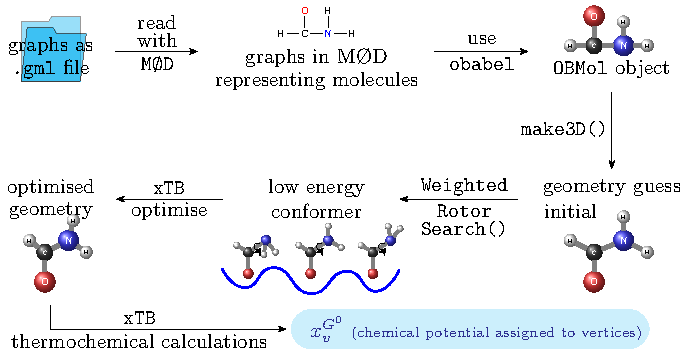
\includegraphics[width=1.1\textwidth]{graphics/chapter3/thermOracle.pdf}
    \vspace{0.5cm}
    \caption{The sequence of operations that was used to assign chemical potentials to the molecules, represented by vertices, in the reaction network, which is referred to thermodynamic oracle in the text.}
    \label{fig: thermOracle}
\end{figure}

The \texttt{.xyz} coordinate file generated by OpenBabel serves as an input file for xTB.
A geometry optimization of the structure is performed with xTB, employing an energy tolerance of $5\times 10^{-8}$ Eh and a gradient tolerance of $5\times 10^{-5}$ Eh bohr$^{-1}$. This is followed by the calculation of the Hessian matrix for the optimized structure, and the chemical potentials at $298.15$ K using standard translational, rotational, vibrational, and electronic partition functions from statistical mechanics under the coupled rigid-rotor and harmonic-oscillator approximations.

\section{On the range of the concentration variable}\label{second appendix}

Apart from the free energies for the molecules, $x^{G^0}_v$, assigned by the thermodynamic oracle the limits on the log concentration values of the molecules, $\left[x^K_v\right]_{\text{min}}$ and $\left[x^K_v\right]_{\text{max}}$ have to be assigned by the user. We provide some comments on the choice of these limits in this work. 
The upper limit for the concentrations is a physical limit bounded by the concentration of the pure substance. Concentration is expressed in the units of moles per liter (mol L$^{-1}$) for liquids and solutions while in terms of partial pressures (in Pa) for gases. For liquids, the maximum possible concentration value of the reactant would be that of the pure liquid, which is physically constrained by
\begin{align*}
    1 \text{ mol of pure liquid} &\equiv M \text{ kg of pure liquid} \\
    1 \text{ mol of pure liquid} &\equiv \frac{M}{\rho} \text{ L of pure liquid} \\
    \text{Maximum concentration} &\equiv \frac{\rho}{M} \text{mol L$^{-1}$}
\end{align*}
For gases, the maximum concentration is imposed by the physical constraint that it has to remain (an ideal) gas following the equation of state $PV = nRT$ so that the equations from the kinetic theory of gases might still be applied to it. The concentration of a gas under some given physical condition of pressure $P$ and temperature $T$ is
\begin{equation*}
    \frac{n}{V} = \frac{P}{RT}
\end{equation*}
As the pressure is increased, or the temperature is deceased to increase the concentration, the gas ceases to behave as an ideal gas and starts exhibiting properties of the vapor phase. A change in the physical state of the substance would have a free energy of phase reaction involved, and it can no longer be modeled only using the equations considered here. 

The lower limit of the reactants is imposed by practical constraints because there are limits to the dilution that can be achieved under laboratory conditions. For a solution, infinite dilution would lead to no solute (reactant) being present, and hence the reaction would not occur. For gases, there are lower limits to pressures that can be achieved in laboratory vacuum settings. Reactions occurring in the solid phase (or on surfaces) are governed by different physical equations and cannot be expressed by this framework. For all practical purposes, we can assume out reactants to be solutions or gases satisfying the condition of a well-stirred reactor.

For this work, we have chosen the limits in the concentration variables as $\left[x^K_v\right]_{\text{min}} = -3$ and $\left[x^K_v\right]_{\text{max}} = 1$. These correspond to physical values of the concentrations between $10^{-3}$ mol lit$^{-1}$ and $10^{1}$ mol lit$^{-1}$. While minimolar concentrations can be achieved under laboratory conditions using standard fludics procedures, a concentration of tens of molars is often encountered for pure liquids (the concentration of pure water is $55.56$ mol lit$^{-1}$). While we use the same range for the log concentration values for all the molecules in the reaction network, the user might choose to assign different ranges for different molecules to make the model more realistic.

\section{Formamide Chemistry}

The primary objective was to study the energetics of condensation pathways of the smaller seed molecules (HCN, NH$_3$, and H$_2$O) into larger oligomers, which might have implication for the prebiotic synthesis of amino acids and compare it with the pathways reported in \cite{implemented_CRN}. 
Therefore, the formulated MILP model was set up to query the pathways with HCN, NH$_3$, and H$_2$O as the input molecules and the trimer of formamide (numbered $17$ in \cite{implemented_CRN}) as the target molecule as shown in Figure~\ref{fig: pathwayQuery}.
The formulated MILP to search for pathways with the given input and output vertices had $336$ variables.

\begin{figure}[!t]
    \centering
    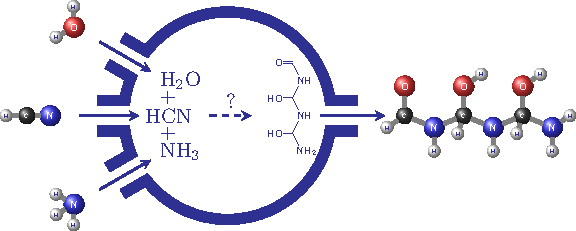
\includegraphics[width=\textwidth]{graphics/chapter3/queryPathway.pdf}
    \vspace{1.0cm}
    \caption{In the generated network, pathways to the target molecule, a trimer of formamide, were queries to with hydrogen cyanide, water and ammonia and source molecules using the method elaborated in Chapter~\ref{ch:thermodynamic_model}.}
    \label{fig: pathwayQuery}
\end{figure}

As a sanity check, the enumerated list of flow solutions returned by the solver included the pathway suggested in \cite{implemented_CRN}, thought not as the optimal solution when scored according to Equation~\eqref{obj_func_impl}.
The sum of free energies of the transitions in this pathway is $-178.412$ kJ mol$^{-1}$, while the sum of free energies weighted by the number of times it is used in the pathway yields $-405.332$ kJ mol$^{-1}$.
This pathway uses four unique transitions (hyperedges) as depicted in Figure~\ref{fig: conventional_path}.
Two of them are used multiple times, which makes seven transitions in total (sum of flows assigned to the hyperedges).
The pathway requires an inflow of three molecules of $v_0$ (hydrogen cyanide) and three molecules of $v_1$ (water) to produce the target molecule $v_5$. The chemical potential $x_v^{\Delta G}$ and the log concentration $x_v^K$ values assigned to each molecule by the MILP solver is listed in Table~\ref{tab:convSoln_molecules}, along with their molecular graphs. The free energy difference of the hyperedges used in the pathway along with the set of vertices which is the inset of the hyperedge (or the reactants in the corresponding transition) is listed under in($v$), while the set of vertices which is the outset of the hyperedge (or the products in the corresponding transition) is listed under out($v$) in Table~\ref{tab:convSoln_reactions}.
\clearpage

\begin{figure}[!t]
    \begin{subfigure}{\textwidth}
        \centering
        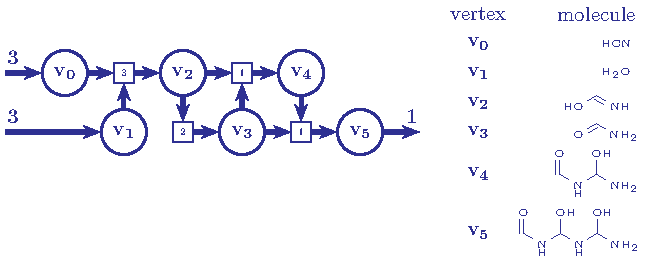
\includegraphics[scale=1.0]{graphics/chapter3/pathway1.pdf}
        \vspace{0.2cm}
        \caption{The pathway reported in \cite{implemented_CRN} with four hyperedges (with the assigned hyperflow the integer in the square) and the molecular graphs for the respective vertices.}
    \label{fig: conventional_path}
    \end{subfigure}
    \vspace{0.5cm}\\
    \begin{subfigure}{\textwidth}
        \centering
        \begin{footnotesize}
		\begin{tabular}{cccrr}
		    \\\toprule
		    vertex & inFlow & outFlow & $x_v^{\Delta G}$ & $x_v^K$ \\
		    \midrule
		    $v_0$ & $3$ & $0$ & $-5.507$ &  $1.000$ \\
		    $v_1$ & $3$ & $0$ & $-5.068$ & $-6.000$ \\
		    $v_2$ & $0$ & $0$ & $-10.610$ & $-6.000$ \\
		    $v_3$ & $0$ & $0$ & $-10.625$ & $0.195$ \\
		    $v_4$ & $0$ & $0$ & $-21.249$ & $-1.190$ \\   
		    $v_5$ & $0$ & $1$ & $-31.869$ & $-6.000$ \\
		    \bottomrule\\
		\end{tabular}
		\end{footnotesize}
		\caption{The inflow for the source molecules and the outflow of the target molecule, along with assignment of the chemical potentials, $x_v^{\Delta G}$, and log concentration, $x_v^K$, of the molecules in the pathway in Figure~\ref{fig: conventional_path}.}
		\label{tab:convSoln_molecules}
    \end{subfigure}
    \vspace{0.5cm}\\
    \begin{subfigure}{\textwidth}
        \centering
        \begin{footnotesize}
		\begin{tabular}{ccccr}
		    \\\toprule
		    hyperedge & $f_e$ & in($v$) & out($v$) & $\overline{x}^{\Delta G}_e$ \\
		    \midrule
		    $e_1$ & $3$ & $v_0, v_1$ & $v_2$ & $-94.141$ \\
		    $e_2$ & $2$ & $v_2$ & $v_3$ & $-38.629$ \\
		    $e_3$ & $1$ & $v_2, v_3$ & $v_4$ & $-0.006$ \\
		    $e_4$ & $1$ & $v_3, v_4$ & $v_5$ & $-45.645$ \\
		    \midrule
		    & & $\sum_e \overline{x}^{\Delta G}_e$ & $=$ & $-178.412$ \\
		    & & $\sum_e f_e\cdot \overline{x}^{\Delta G}_e$ & $=$ & $-405.332$ \\
		    \bottomrule\\
		\end{tabular}
		\end{footnotesize}
		\caption{The MILP solution assigns hyperflows $f_e$ to the hyperedges in the pathway from Figure~\ref{fig: conventional_path}.}
		\label{tab:convSoln_reactions}
    \end{subfigure}\\
    \vspace{0.5cm}
    \caption{Details of the pathway reported in \cite{implemented_CRN}. The $x_v^{\Delta G}$ values are in atomic units (Hartrees), the $x_v^K$ values are the dimensionless equivalent of $\log_{10} \frac{[\text{conc.}]}{1 \text{ mol lit}^{-1}}$, where conc. is the concentration of the molecule in mol lit$^{-1}$ while $\overline{x}^{\Delta G}_e$ are in kJ mol$^{-1}$.}
\end{figure}


\begin{figure}[!t]
    \begin{subfigure}{\textwidth}
        \centering
        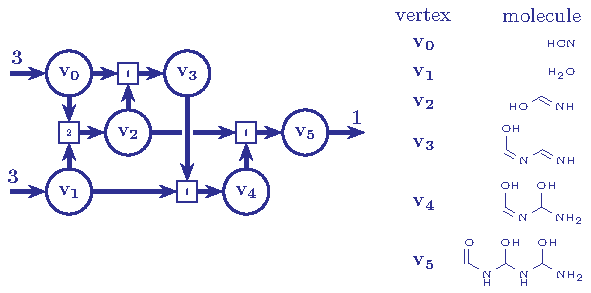
\includegraphics[scale=1.0]{graphics/chapter3/pathway2.pdf}
        \vspace{0.2cm}
        \caption{The best scoring pathway with four hyperedges and the molecular graphs for the respective vertices.}
    \label{fig: shortest_path}
    \end{subfigure}
    \vspace{0.5cm}\\
    \begin{subfigure}{\textwidth}
        \centering
        \begin{footnotesize}
		\begin{tabular}{cccrr}
		    \\\toprule
		    vertex & inFlow & outFlow & $x_v^{\Delta G}$ & $x_v^K$ \\
		    \midrule
		    $v_0$ & $3$ & $0$ & $-5.507$ &  $1.000$ \\
		    $v_1$ & $3$ & $0$ & $-5.068$ & $-6.000$ \\
		    $v_2$ & $0$ & $0$ & $-10.610$ & $1.000$ \\
		    $v_3$ & $0$ & $0$ & $-16.159$ & $-6.000$ \\
		    $v_4$ & $0$ & $0$ & $-21.240$ & $1.000$ \\        
		    $v_5$ & $0$ & $1$ & $-31.869$ & $-6.000$ \\
		    \bottomrule\\
		\end{tabular}
		\end{footnotesize}
    	\caption{The inflow for the source molecules and the outflow of the target molecule, along with assignment of the chemical potentials, $x_v^{\Delta G}$, and log concentration, $x_v^K$, of the molecules in the pathway in Figure~\ref{fig: shortest_path}.}
		\label{tab:shortestSoln_molecules}
    \end{subfigure}
    \vspace{0.5cm}\\
    \begin{subfigure}{\textwidth}
        \centering
        \begin{footnotesize}
		\begin{tabular}{ccccr}
		    \\\toprule
		    hyperedge & $f_e$ & in($v$) & out($v$) & $\overline{x}^{\Delta G}_e$ \\
		    \midrule
		    $e_1$ & $2$ & $v_0, v_1$ & $v_2$ & $-94.141$ \\
		    $e_2$ & $1$ & $v_0, v_2$ & $v_3$ & $-129.554$ \\
		    $e_3$ & $1$ & $v_1, v_3$ & $v_4$ & $-38.298$ \\
		    $e_4$ & $1$ & $v_2, v_4$ & $v_5$ & $-51.185$ \\
		    \midrule
		    & & $\sum_e \overline{x}^{\Delta G}_e$ & $=$ & $-313.178$ \\
		    & & $\sum_e f_e\cdot \overline{x}^{\Delta G}_e$ & $=$ & $-407.319$ \\
		    \bottomrule\\
		\end{tabular}
		\end{footnotesize}
		\caption{The MILP solution assigns hyperflows $f_e$ to the hyperedges in the pathway from Figure~\ref{fig: shortest_path}.}
		\label{tab:shortestSoln_reactions}
    \end{subfigure}\\
    \vspace{0.5cm}
    \caption{Details of the best scoring pathway on applying the model proposed in Chapter~\ref{ch:thermodynamic_model} along with the objective function (8). The units are the same as in Table~\ref{tab:convSoln_reactions}.}
\end{figure}

While thermodynamics might provide an insight to the equilibrium flows in the reaction network,
it does not describe the path to that equilibrium.
Each transition has an associated barrier energy that must be overcome for the transition to occur.
Enumerating pathways using our implementation of the MILP formulation of the problem provides the pathway in Figure~\ref{fig: shortest_path} as one with the minimum value of the objective function.
This pathway utilizes four unique transitions and five transitions in all to realize the pathway,
which is fewer than the previously reported pathway.
Since the difference in the chemical potential between the source and target molecules is fixed,
choosing hyperedges with larger free energy differences would increase the value of the objective function.
Using transition with larger free energy differences to `cover' the net difference in the chemical potential,
lead to fewer transitions being used in the pathway. 

The main source of difference in the objective function value in the two pathways is the chemical potential of the molecule $v_3$ from Figure~\ref{fig: shortest_path} that is not present in the conventional pathway.
While the conventional pathway in~\cite{implemented_CRN} is more symmetric and appealing because of the stepwise nucleophilic attack on the carbonyl $C$ atom by the amine $N$ atom of an adjacent $v_3$ molecule, which is repeated twice to generate $v_5$ as illutrated in Figure~\ref{fig: symAdd}, \cite{implemented_CRN} also notes that these condensation reactions have a positive Gibbs free energy.

\begin{figure}[!t]
	\begin{subfigure}{\textwidth}
        \centering
        \vspace{0.2cm}
        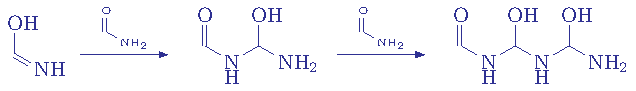
\includegraphics[scale=1.0]{graphics/chapter3/symAdd.pdf}
        \vspace{0.2cm}
    	\caption{Stepwise trimerization of formamide by iterative addition of the monomer as hypothesised in the conventional pathway shown in Figure~\ref{fig: conventional_path}.}
    	\label{fig: symAdd}
    \end{subfigure}\\
    \vspace{0.5cm}
    \begin{subfigure}{\textwidth}
        \centering
        \vspace{0.2cm}
        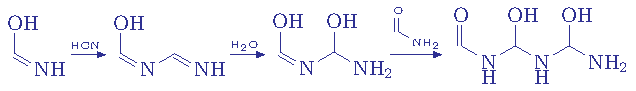
\includegraphics[scale=1.0]{graphics/chapter3/stepAdd.pdf}
        \vspace{0.2cm}
        \caption{The trimerization of formamide which uses $v_3$ in the pathway that is returned as the best scoring pathway as shown in Figure~\ref{fig: shortest_path}.}
        \label{fig: stepAdd}
    \end{subfigure}
    \caption{The difference between the best-scoring pathway returned by the proposed method and the pathway hypothesised in~\cite{implemented_CRN}.}
\end{figure}

To quote the authors, 
\begin{quote}
`\emph{each step is endergonic although decreasingly so.
Dimerization of formamide is uphill 19.8 kcal/mol, owing to the thermodynamic stability of the monomers in solution.
Addition of another monomer to form the trimer, via similar nucleophilic attack, is uphill 19.0 kcal/mol}'.
\end{quote}
This can also be observed in the ILP solution in Table~\ref{tab:convSoln_reactions} for the conventional pathway where the hyperedges $e_3 \equiv (\{v_2, v_3\}, \{v_4\})$ have a $\overline{x}_e^{\Delta G}$ value close to zero.
The constraint in Equation~\eqref{proposed_constraint3} forces the hyperedge to have $\overline{x}_e^{\Delta G} \leq 0$ for it to be included in the pathway.
The MILP solver chooses the log concentration variables $x_v^K$ for the molecules $v_3$ and $v_4$ in such a way so that $\overline{x}_e^{\Delta G}$ variables for $e_3$ is just below zero to realize the pathway.
This might be the reason for $x_v^K$ for these two vertices not having the extremal value as is often the case, as discussed below.
Our proposed model also returns an alternative pathway involving $v_3$ from Figure~\ref{fig: stepAdd}, where none of the $\overline{x}_e^{\Delta G}$ weights for the hyperedges is close to zero as listed in Table~\ref{tab:shortestSoln_reactions}.

We observe that the log concentration variables are always assigned extremal values decided by the constraint in Equation~\eqref{proposed_constraint8}.
This is likely an artifact of using an MILP solver with an objective function for the problem.
An MILP is a convex optimization problem where minimizing the objective function (involving a subset of the MILP variables) results in a solution located at a vertex of the convex space defined by the constraints.
The bounds for the variables are hand-crafted by the user and it might be more realistic to assign different bounds for the log concentration variable for each vertex.
Alternatively, a better interpretation of the assigned values for the variables, $x_v^K$ might be the direction in which the equilibrium concentrations have to be perturbed to achieve the desired flow.
For example, the concentration values in Table~\ref{tab:convSoln_molecules} can be interpreted as the concentrations of $v_1$, $v_3$ and $v_5$ have to be lowered and the concentrations of $v_0$, $v_2$ and $v_4$ have to be raised to achieve a larger difference in the potentials while effecting a net outflow of molecule $v_5$ given input molecules $v_0$ and $v_1$. 

\begin{table}[!t]
    \centering
    \begin{footnotesize}
    \begin{tabular}{ccccrrr}
        \\\toprule
        \# & $\sum_{e} f_e$ & $\sum_{e} z_e$ & $|v|$ & \hspace{0.1cm}obj \eqref{obj_func_impl} & $\sum_{e} f_e \cdot x_e^{\Delta G}$ & rxn sequence \\
        \midrule
        0 & $5$ & $4$ & $6$ & $-305.697$ & $-399.837$ & $1,3,4,10$ \\
        1 & $6$ & $5$ & $7$ & $-306.697$ & $-399.837$ & $1,3,4,5,9$ \\
        2 & $6$ & $5$ & $7$ & $-305.696$ & $-399.836$ & $1,2,3,4,11$ \\

		3 & $5$ & $3$ & $5$ & $-211.555$ & $-399.836$ & $1,6,9$ \\   
		4 & $5$ & $3$ & $5$ & $-211.554$ & $-399.836$ & $1,8,10$ \\
		5 & $6$ & $4$ & $6$ & $-211.556$ & $-399.836$ & $1,8,5,9$ \\
        6 & $6$ & $4$ & $6$ & $-211.556$ & $-399.836$ & $1,2,7,9$ \\     
        7 & $6$ & $4$ & $6$ & $-211.554$ & $-399.836$ & $1,2,8,11$ \\
        \bottomrule\\
    \end{tabular}
    \end{footnotesize}
    \caption{All enumerated pathways to the target molecule in the network, with the sequence of pathways leading to the target molecules. The specific reactions corresponding to the index listed in the sequence of reactions for each pathway listed in the last column can be read from Figure~\ref{fig: rxnList}. }
    \label{tab: thermo_flow}
\end{table}

An exhaustive search of the reaction space led to the identification of $13$ distinct reaction pathways \cite{solutions_data}, listed in Table~\ref{tab: thermo_flow} in the order of increasing value of objective \ref{obj_func_impl}. The column list the rank, the total number of reactions used, the number of unique reactions used, the number of molecules involved, the value of the objective \eqref{obj_func_impl} and the sum of the free energy differences of the reactions weighted by the flows in the columns respectively. Note, that the second column from the right gives the net free energy difference, which is path independent and therefore, the same for all the listed pathways. These pathways were enumerated in $866$ seconds on an AMD$^{\circledR}$ Ryzen 5 PRO 4650U CPU (2.1 GHz) utilizing $8$ threads. One may consult the list of reactions in Figure~\ref{fig: rxnList} for the molecules and the exact set of reactions involved in these pathways.

\begin{figure}[!t]
    \centering
    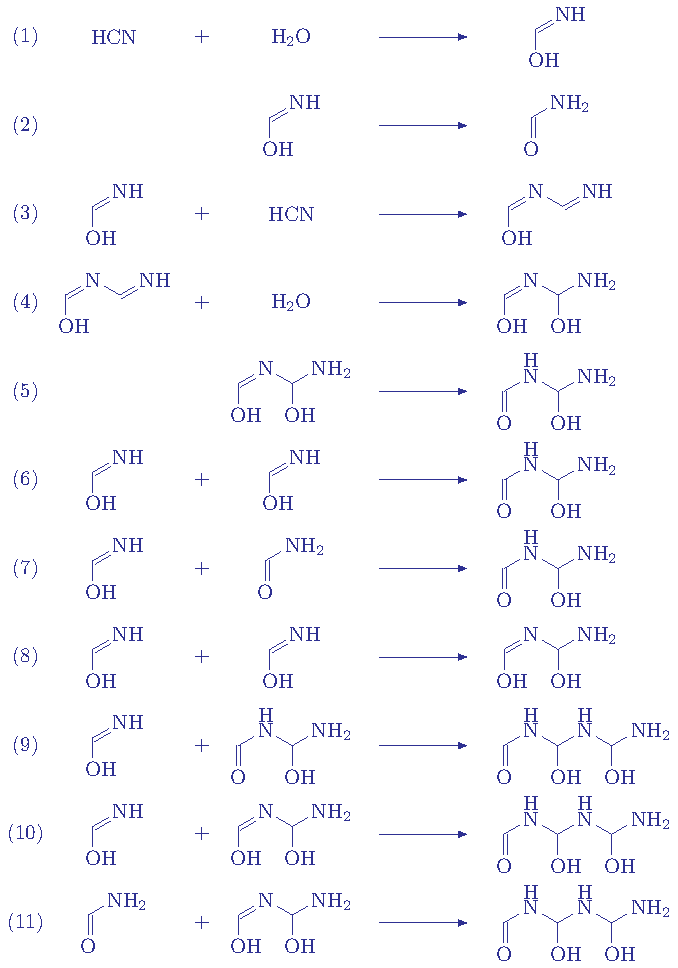
\includegraphics[scale=1.0]{graphics/chapter3/rxnList.pdf}
    \vspace{0.5cm}
    \caption{The list of the reactions used in the pathways to the target molecules, with the sequence of specific reactions in each pathway listed in Table~\ref{tab: thermo_flow}.}
    \label{fig: rxnList}
\end{figure}

\begin{refsection}

%************************************************
\chapter{Refinements to the model}
\label{ch:refined_model} %
%************************************************

{\sffamily\slshape The text in this chapter is identical to Section 3 of the published version of the preprint at \href{https://arxiv.org/abs/2504.10609}{arXiv:2504.10609} along with some additional figures.\\}

In this chapter, we develop an objective measure to rank pathways in a reaction network maximizing the probability of the entire pathway based on physical principles. 
Additionally, based on the notion that energy barriers of reactions are the determining factor for the kinetics of the network, we develop an automated methodology for computing such energy barriers, building on a combination of an array of existing computational tools. A key novelty is that in contrast to the standard manual intervention required to generate reaction trajectories from which the reaction barrier can be estimated, we try to automate this part of the process.
Lastly, we formulate an integer linear program which allows the user to specify queries for pathways in the network in a very flexible and generic way. Solving this integer linear program returns all pathways fulfilling the criteria, ranked by the objective measure mentioned above.
In short, this gives an automated, general, and flexible methodology for analyzing reaction networks, a methodology which offers a speed-up over manual search for pathways but with comparable quality.

In this chapter, we detail our proposed methodology for automating the search for kinetically informed pathways in reaction networks. As shown in Figure~\ref{fig: thermoEnergyBarrierCases}, the kinetics of the reaction can often lead to different results than those obtained from the reaction thermodynamics as done in Chapter~\ref{ch:thermodynamic_model}. In Sections~\ref{reaction_prob} and \ref{obj_func}, we first propose an objective function for ranking pathways in a reaction network annotated with kinetic data in the form of energy barriers for each reaction. In Section~\ref{implemented_model}, we then formulate an integer linear program (ILP) representing such networks and allowing the specification and execution of pathway searches. This part builds on the modeling described in Chapter~\ref{ch:thermodynamic_model}. We also describe how to search for not only one, but multiple solutions to a given pathway query, ordered by an objective function such as the one presented in Section~\ref{obj_func}. 

\newpage
\begin{figure}[!htb]
    \centering
    \begin{subfigure}{0.8\textwidth}
        \centering
        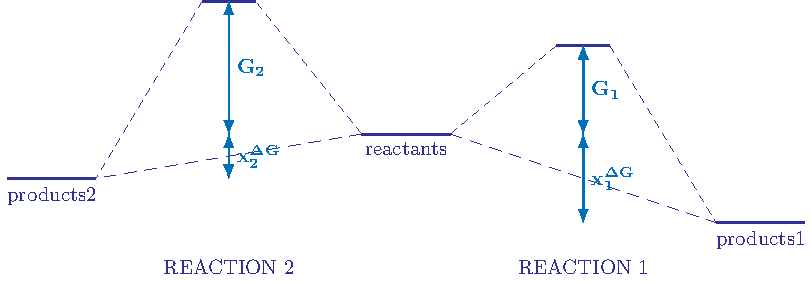
\includegraphics[width=\textwidth]{graphics/chapter4/case1.pdf}
        \caption{the thermodynamically more favored reaction are generally also kinetically preferred.}
        \label{fig: case1}
    \end{subfigure}
    \\
    \begin{subfigure}{0.8\textwidth}
        \centering
        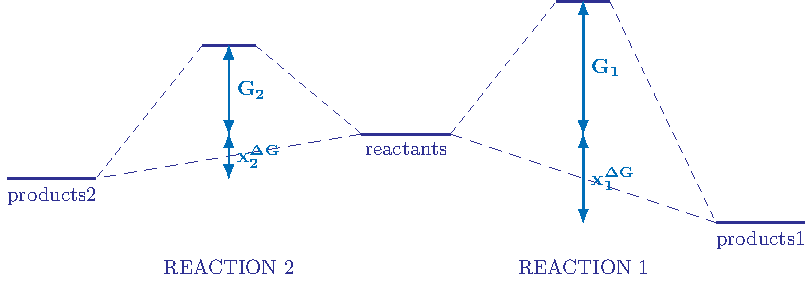
\includegraphics[width=\textwidth]{graphics/chapter4/case2.pdf}
        \caption{the thermodynamically less favored reaction with a smaller negative Gibbs free energy difference is also kinetically preferred because it has a lower energy barrier.}
        \label{fig: case2}
    \end{subfigure}
    \\
    \begin{subfigure}{0.8\textwidth}
        \centering
        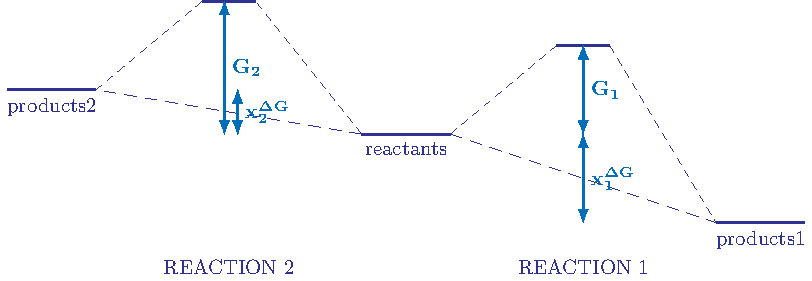
\includegraphics[width=\textwidth]{graphics/chapter4/case3.pdf}
        \caption{the thermodynamically unfavored reactions (with a positive Gibbs free energy difference) generally have higher energy barriers and are kinetically not preferred.}
        \label{fig: case3}
    \end{subfigure}
    \\
    \begin{subfigure}{0.8\textwidth}
        \centering
        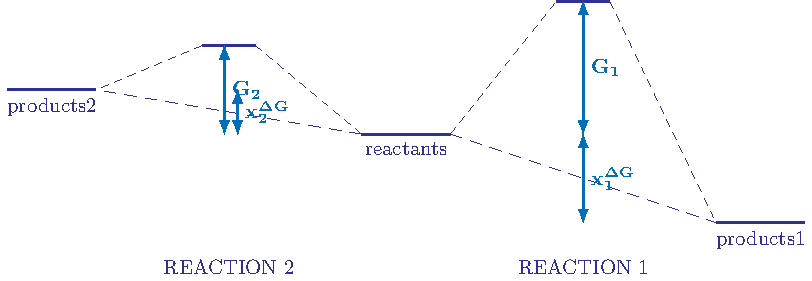
\includegraphics[width=\textwidth]{graphics/chapter4/case4.pdf}
        \caption{however, in fringe cases a thermodynamically unfavored reaction might have a lower energy barrier than a thermodynamically favored reaction.}
        \label{fig: case4}
    \end{subfigure}
    \vspace{0.2cm}
    \caption{Four of the many possible cases where the thermodynamics and kinetics of reactions might lead to different results. In cases \ref{fig: case2} and \ref{fig: case4}, the results based on thermodynamics are expected to be different from those obtained from kinetics.}
    \label{fig: thermoEnergyBarrierCases}
\end{figure}
\newpage


\section{From Rate Constants to Edge Weights}
\label{reaction_prob}

Irrespective of whether one uses Arrhenius' theory \cite{arrhenius1,arrhenius2}, collision theory or transition state theory \cite{eyring_equation}, the dependence of the rate constant~$k_e$ of a reaction~$e$ on the free energy barrier $G_e$ follows that of a negative exponential. The expression for the rate constant by Eyring's equation from transition state theory is
\begin{equation}
    k_e = \frac{k_b T}{h} \exp\left(-\frac{G_e}{RT}\right) \label{energy_barrier}
\end{equation}
where $R$ is the universal gas constant, $k_b$ is the Boltzmann constant, and $h$ is the Planck constant, each in their appropriate units.
In a well-stirred system where all the reactions in the reaction network are assumed to be concurrently taking place, the temperature can be considered to be the same for all reactions. Hence, it is not a factor affecting the relative rates of the reactions in the system.

Since our modeling is not aimed at capturing temporal changes in the concentrations of molecules, we make the simplifying assumption that all molecules in the reaction network are present with unit concentrations. 
This avoids the time propagation of the changes in the concentration of the molecules, as some of then a used up as reactants to produce other molecules.  
Under this assumption, the rate constant $k_e$ can be interpreted as being proportional to the probability of reaction~$e$ happening in a fixed small volume and time interval. 
A reaction with a higher rate constant (and lower energy barrier) is expected is occur more frequently, hence the probability of that reaction occurring in a fixed interval of time when a limited number of reactant molecules are present would be higher.
To interpret the rate constant as probabilities of the reaction in a given reaction network, we normalize these values to sum to one:
\begin{align}
    p(e) &= \frac{k_e}{\sum_{i\in E} k_i} \nonumber \\ 
    &= \frac{\frac{k_b T}{h} \exp\left(-\frac{G_e}{RT}\right)}{\sum_{i\in E} \frac{k_b T}{h} \exp\left(-\frac{G_i}{RT}\right)}\tag{\text{using }\ref{energy_barrier}} \\
    &= \frac{\frac{k_b T}{h} \exp\left(-\frac{G_e}{RT}\right)}{\frac{k_b T}{h} \sum_{i\in E} \exp\left(-\frac{G_i}{RT}\right)} \nonumber \\
    &= \frac{\exp\left(-\frac{G_e}{RT}\right)}{\sum_{i\in E} \exp\left(-\frac{G_i}{RT}\right)} \nonumber \\
    &= \frac{\exp\left(-\frac{G_e}{RT}\right)}{D} \label{prob_reaction}
\end{align}

Here, the denominator $\sum_{i\in E} \exp(-\frac{G_i}{RT})$ is the same for all reactions~$e$ and has been shortened to~$D$. In the current work, we assign the measure~$p(e)$ as the weight of the hyperedge representing~$e$ in an attempt to score reactions with lower energy barriers favourably.
However, the user is free to assign any other measures of weight to the hyperedges in the reaction network, if deemed better suited for a particular pathway search objective.

Figure~\ref{fig:twoReactions} tries to illustrate the reasoning behind assigning the weight measure to the respective reactions. There are two reactions with energy barriers $G_1$ and $G_2$ with $G_2 > G_1$ as shown in Figure~\ref{fig:two_reactions}. The energy distribution of the reactant molecules for both the reactions is given by the Maxwell-Boltzmann energy distribution in Figure~\ref{fig:boltzmannProfile}, and the fraction of molecules with the available energy to overcome the energy barrier of the respective reaction and form the products is given by
\begin{align*}
	f(N) &= \int_{G_i}^\infty P(E)\, dE \\
	&\sim \int_{G_i}^\infty \exp\left(-\frac{E}{RT}\right)\, dE \\
	&= \exp\left(-\frac{G_i}{RT}\right)
\end{align*}

\begin{figure}[!t]
    \centering
    \begin{subfigure}{0.9\textwidth}
        \centering
        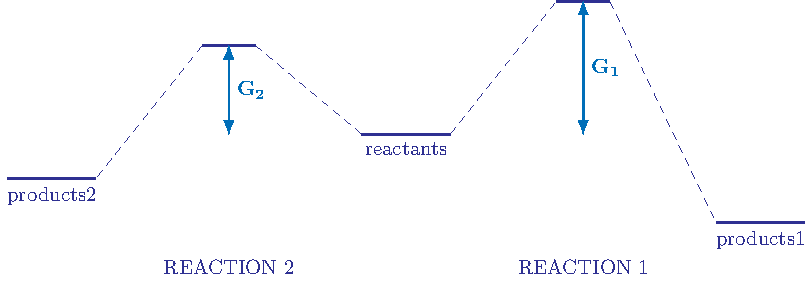
\includegraphics[width=\textwidth]{graphics/chapter4/twoReactions.pdf}
        \caption{Reactions with different energy barriers compete for the limited reactant molecules to form the respective products.}
        \label{fig:two_reactions}
    \end{subfigure}
    \vspace{0.5cm}
    \\
    \begin{subfigure}{0.9\textwidth}
        \centering
        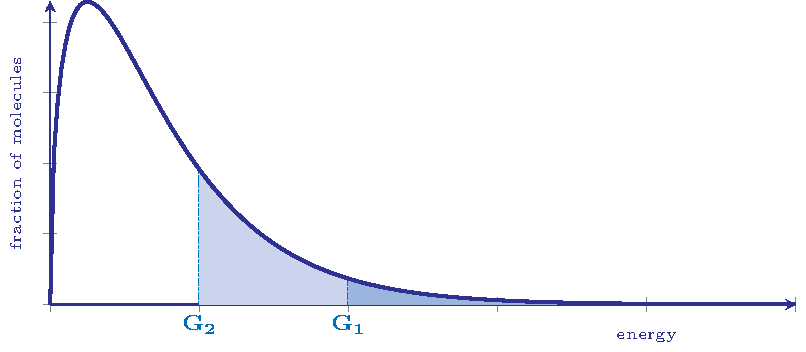
\includegraphics[width=\textwidth]{graphics/chapter4/twoReactionsNumberDensity.pdf}
        \caption{The reaction with the lower energy barrier is accessible to a larger fraction of the reactant molecules as more molecules have the energy required to form the products (denoted the shaded area under the curve).}
        \label{fig:boltzmannProfile}
    \end{subfigure}
    \caption{Of the two reactions competing for the same reactant molecules, the one with a lower energy barrier is favored as more reactant molecules can form the products. Therefore, it has a higher rate (given by Equation~\eqref{energy_barrier}) and assigned a higher probability of occurring by Equation~\eqref{prob_reaction} in a finite time with limited number of reactant molecules.}
    \label{fig:twoReactions}
\end{figure}

The rate of the reaction would be expected to be proportional to this fraction of molecules with enough energy to form the respective products, and might therefore, be used as a weight on a reaction to score its inclusion in the pathway. A pathway consisting of reactions with lower energy barriers would be scored higher as a larger fraction of molecules would overcome each reaction in the pathway. 

\section{Formulating an Objective Function}
\label{obj_func}

\begin{figure}[t]
    \centering
    \begin{subfigure}{\textwidth}
        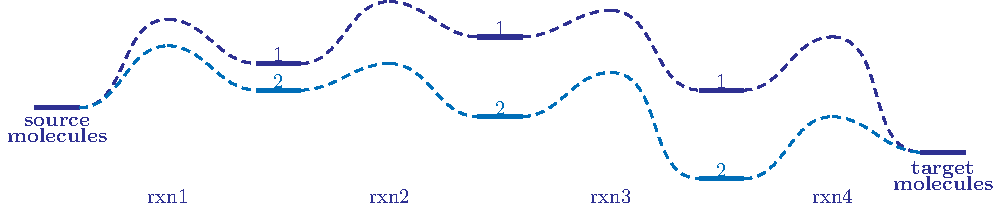
\includegraphics[scale=0.6]{graphics/chapter4/objFunc1.pdf}
        \caption{such a pathway 2 would be clearly more favored than pathway 1.}
        \label{fig: objFunc1}
    \end{subfigure}
    \vspace{0.2cm}
    \\
    \begin{subfigure}{\textwidth}
        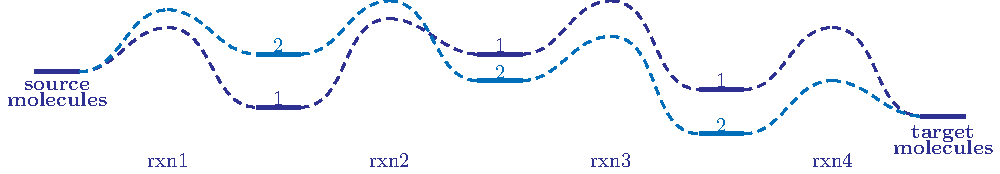
\includegraphics[scale=0.6]{graphics/chapter4/objFunc2.pdf}
        \caption{it is difficult to decide which of the pathways is more favored because not all molecules in one pathway have higher energies than the other (the energy profiles of the pathways cross at the second reaction).}
        \label{fig: objFunc2}
    \end{subfigure}
	\vspace{0.2cm}
    \\
    \begin{subfigure}{\textwidth}
        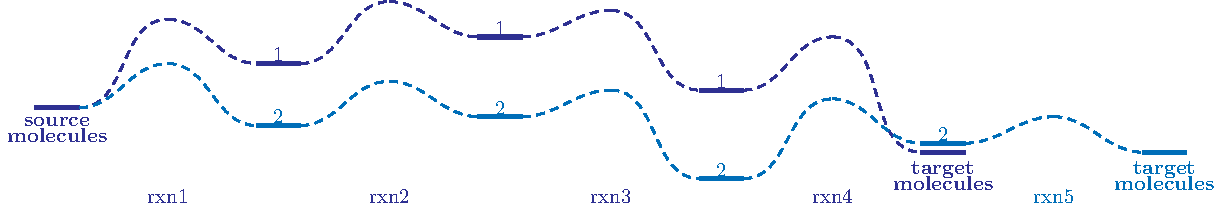
\includegraphics[scale=0.6]{graphics/chapter4/objFunc3.pdf}
        \caption{it is also difficult to decide if pathway 1 (a shorter pathway with $4$ reactions but higher barriers) is more favourable than pathway 2 (a longer pathway with $5$ reactions but lower barriers).}
        \label{fig: objFunc3}
    \end{subfigure}
    \caption{An objective function scores pathways and helps to decide which would be more favourable when it is not obvious such as in the cases depicted in~\ref{fig: objFunc2} and~\ref{fig: objFunc3}.}
    \label{fig: objFuncCases}
\end{figure}

We are interested in pathways from the given source molecules to the desired target molecule(s) that have a high overall probability of occurring in practice. This might not always be easy to determine when there are multiple pathways to the target molecule(s) as shown in Figure~\ref{fig: objFuncCases}. Considering individual reactions in a pathway as independent events (and abusing the notation~$e$ to mean the event of reaction~$e$ happening), the probability~$p_{\text{total}}$ of the entire set of reactions in the pathway occurring in one unit of time and one unit of volume is
\begin{align*}
    p_{\text{total}} &= p\left( \bigwedge_{e: f_e > 0} \left(e\wedge e \wedge \ldots f_e\text{ times}\right)\right) \\
    &= \prod_{e: f_e > 0} p(e)^{f_e} \\
    &= \prod_{e: f_e > 0} \left[\frac{\exp\left(-\frac{G_e}{RT}\right)}{D}\right]^{f_e} \tag{\text{using }\ref{prob_reaction}} \\
    &= \frac{\prod_{e: f_e > 0} \exp\left(-\frac{f_e\cdot G_e}{RT}\right)}{\prod_{e: f_e > 0} D^{f_e}} \\
    &= \left.\exp\left(-\frac{\sum_{e \in E} f_e\cdot G_e}{RT} \right) \middle/ D^{\sum_{e \in E} f_e}\right.
\end{align*}
Since the energy barrier $G_e$ is weighted by the flow $f_e$, the conditional sum $e: f_e > 0$ can be substituted by a simple sum over all hyperedges $e\in E$ because hyperedges with $f_e = 0$ do not contribute to the value of the sum.
The expression for the total probability of a pathway is a fraction and we take the logarithm of it to simplify it and make it a linear expression.
\begin{align*}
    \log p_{\text{total}} &= \log \left[\exp\left(-\frac{\sum_{e \in E} f_e\cdot G_e}{RT} \right) \middle/ D^{\sum_{e \in E} f_e}\right] \\
    &= -\frac{\sum_{e \in E} f_e\cdot G_e}{RT} - \left(\sum_{e \in E} f_e\right) \cdot \log D 
\end{align*}
The last line is proportional to the following expression obtained by multiplying by $RT$
\begin{equation*}
    -\sum_{e \in E} f_e\cdot G_e - RT\cdot \log D\cdot \sum_{e \in E} f_e
\end{equation*}
The probability of the set of reactions in the pathway is then maximized by maximizing the value of the obtained expression:
\begin{equation*}
    \max\left(-\sum_{e \in E} f_e\cdot \left(G_e + RT\cdot \log D \right)\right)
\end{equation*}
This is equivalent to the following minimization problem:
\begin{align}
    \min\left(\sum_{e \in E} f_e\cdot \left(G_e + RT\cdot \log D \right)\right) \label{proposed_objective}
\end{align}
This proposed objective value~\eqref{proposed_objective} is a linear expression because the $G_e$'s are constants from the input instance, $T$ is assumed constant, and $R$ is a physical constant. Also, the value $\log D = \log \left(\sum_{i\in E} \exp\left(-\frac{G_i}{RT}\right)\right)$ is constant when considering a fixed reaction network.

We note that via $D$, the objective value~\eqref{proposed_objective} of a pathway will depend on the underlying reaction network in which it is considered embedded. This may be regarded as a weakness. On the other hand, the objective value \eqref{proposed_objective} is intuitively appealing by being composed of two natural components: Its first component $\sum_{e \in E} f_e\cdot G_e$ favors pathways with small sums of energy barriers of the reactions in the pathway, weighted by the number of times it is used. Its second component $\sum_{e \in E} f_e \cdot \left( RT \, \log D\right)$ favors pathways with fewer reactions. The factor $ RT \log D$ can be viewed as weighting the relative importance of the two components and decides which of the two pathways is more favourable in cases such as the one shown in Figure~\ref{fig: objFunc3}.

\section{ILP Modeling} \label{implemented_model}

In this section, we express the modeling of Chapter~\ref{ch:toolbox} as an integer linear program (ILP). Recall the key idea that in a reaction network, pathways can be expressed as hyperflows and pathway queries can be expressed as constraints on hyperflows. Such constraints can simply be added to the ILP, after which the pathway queries can be executed by running an ILP-solver on the final ILP. We also describe how to search for multiple, structurally different solutions to a given pathway query, ordered by an objective function such as~\eqref{proposed_objective}.

Thus, in the ILP a pathway is represented by a vector of non-negative\footnote{Non-negative flow values require reversible reactions to be modeled as two separate hyperedges in the reaction network, but it also allows the flexibility to model some reactions as irreversible.} integer-valued variables~$f_e$, one variable for each reaction~$e$ in the reaction network. These flow variables are subject to the key constraint~\eqref{int_hyperflow_jakob}, as well as to the user-supplied constraints that specify the pathway query under consideration.

To model reversible reactions, separate hyperedges were added for the forward and backward directions of the reaction. This allows us to restrict the flows to non-negative integers only. The use of the reverse of a reaction would be denoted by a positive flow on the hyperedge in the opposite direction.
\begin{equation}
    f_e \geq 0 \tag{\ref{proposed_constraint2}}
\end{equation}

For each reaction~$e$, we add a boolean indicator variable $z_e$ which keeps track of whether the hyperedge~$e$ is used in the pathway or not. The values of these variables are assigned according to their respective flow variables following the biimplication constraints:
\begin{align}
    f_e = 0 &\iff z_e = 0 \tag{\ref{biimp3}} \\
    f_e \geq 1 &\iff z_e = 1 \tag{\ref{biimp4}}
\end{align}
We will use these indicator variables later when listing multiple, structurally different solutions to a given pathway query as elaborated in Section~\ref{enumerateSolutions} and for assigning a partial order to vertices in the pathway as elaborated in Section~\ref{partial_order}.\footnote{The indicator variables can also increase expressiveness when specifying pathway queries.} Many ILP solvers support addition of such indicator constraints \eqref{biimp1} and \eqref{biimp2} directly as implications to an ILP problem (which are then solved by a nonlinear, nonconvex reformulation of the indicator constraint). If this feature is not available, one can instead use the method of linearizing these implication constraints via a large constant~$M$.

\begin{table}[t]
    \centering
    \begin{scriptsize}
    \begin{tabular}{ccr}
        \toprule
        Constant & Datatype & Description \\
        \midrule
        $G_e$ & float & Weight of the hyperedge $e$ \\[1mm]
        $s_{ve}^+$ & integer & Count of molecule $v$ \\
        && on the LHS of a reaction $e$ \\[1mm]
        $s_{ve}^-$ & integer & Count of molecule $v$ \\
        && on the RHS of a reaction $e$ \\[1mm]
        $RT$ & float & Product of \\
        && universal gas constant \\
        && and temperature \\[1mm]
        $M$ & integer & Big integer used for \\
        && linearizing the constraints \\
        && (type promoted to float,\\
        && if required) \\
        \bottomrule
    \end{tabular}
    \end{scriptsize}
    \caption{Constants in the proposed ILP formulation.}
    \label{tab: ILP constants}
\end{table}%

\begin{table}[!h]
    \centering
    \begin{scriptsize}
    \begin{tabular}{ccr}
        \toprule
        ILP variable & Datatype & Description \\
        \midrule
        $f_e$ & integer & Flow variable for\\
        && a hyperedge $e$ \\
        && non-negative \\[1mm]
        $z_e$ & boolean & Indicator variable \\
        && denoting if a hyperedge \\
        && $e$ is used in the flow \\
        \bottomrule
    \end{tabular}
    \end{scriptsize}
    \caption{Variables in the proposed ILP formulation.}
    \label{tab: ILP variables}
\end{table}%

In summary, the resulting ILP looks as follows:

\begin{align}
    & \min\left(\sum_{e \in E} \left(f_e\cdot G_e + RT\cdot \log D\cdot f_e\right)\right) \tag{\ref{proposed_objective}} \\
    \forall e \in E\colon & 0 \leq f_e \tag{\ref{proposed_constraint2}} \\
    \forall v\in V \colon &\sum_{ e\in \overline{E} } s_{ve}^+ f_e - \sum_{ e\in \overline{E} } s_{ve}^- f_e = 0 \tag{\ref{int_hyperflow_jakob}}\\
    &\text{Constraints specifying the pathway query} \nonumber\\
    &\text{such as, inflow and outflow constraints} \nonumber\\
    & f_e = 0 \iff z_e = 0 \tag{\ref{biimp3}} \\
    & f_e \geq 1 \iff z_e = 1 \tag{\ref{biimp4}}
\end{align}

The constraints specifying the pathway consist of the desired outflow of the queried target molecule and the supplied source molecules. Additionally, it might involve constraints such an disallowing particular molecules as by-products (by restricting their outflow to zero), or disallowing the use of particular reactions (by specifying $f_e = 0 = z_e$ for those reactions). An overview of the variables and constants in the ILP can be found in Table \ref{tab: ILP variables} and \ref{tab: ILP constants}, respectively.

\subsection{Enumeration of solutions}
\label{enumerateSolutions}

\begin{figure}[t]
    \centering
    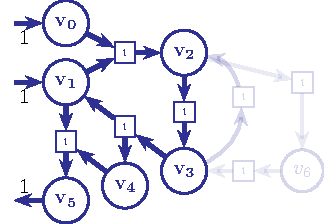
\includegraphics[scale=1.5]{graphics/chapter4/null_cycle.pdf}
    \caption{An example of a solution (the hyperflow of the entire figure) which contains a previous solution (the hyperflow shown in solid blue) as a subset, seen in terms of the edges (reactions) used. 
    Adding the faded hyperedges to the integer hyperflow depicted in solid blue creates a `null cycle' which creates a hyperflow solution that satisfies constraint~\eqref{int_hyperflow_jakob} but does not create a physically different solution.
    Addition of constrain~\eqref{subset_elimination} for all previously returned solutions ensures that such solutions are not returned.} 
    \label{fig: cover}
\end{figure}

We would like to enumerate multiple solutions to a pathway query in the reaction network. In this enumeration, we prefer to get a diverse set of pathways, in order to make the result more robust to uncertainties in the weights (i.e., the energy barrier values) assigned to the hyperedges. 
Such diversity offers a selection of alternative pathways for implementation, which is beneficial in case the single optimal solution turns out to be unattainable in practice (or just less desirable than expected due to circumstances not included in the modeling).
Some ILP solvers provide so-called solution pools which allow enumeration of solutions, but the process of populating this pool of solutions is often opaque.
More control is given in M{\O}D~\cite{mod_web}, which provides an option to enumerate multiple solutions based on a user-supplied specification of which subset of integer and binary variables to enumerate over~\cite{jakob_integer_hyperflows}.
For example, if the specification lists exactly the variables $z_e$ for each $e\in E$, then two pathways using the same set of hyperedges (but potentially with a difference in the flow value on some edges) will be considered equal,
and only the one with the best objective value is returned.
That is, if we define $supp(f) = \{e\in E \mid z_e = 1\}$ then two solutions $f_1$ and  $f_2$ are considered different exactly when $supp(f_1) \neq supp(f_2)$.

\begin{figure}[!h]
    \centering
    \begin{subfigure}{0.8\textwidth}
        \centering
        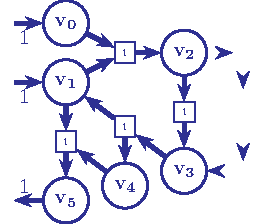
\includegraphics[scale=1.4]{graphics/chapter4/subset1.pdf}
        \vspace{0.5cm}
        \caption{An integer hyperflow solution with $4$ hyperedges.}
        \label{fig:solution1}
    \end{subfigure}
    \vspace{1cm}
    \\
    \begin{subfigure}{0.8\textwidth}
        \centering
        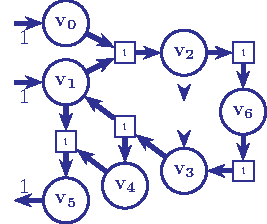
\includegraphics[scale=1.4]{graphics/chapter4/subset2.pdf}
        \vspace{0.5cm}
        \caption{Another integer hyperflow solution to the same flow query using $5$ hyperedges.}
        \label{fig:solution2}
    \end{subfigure}
    \vspace{1cm}
    \\
    \begin{subfigure}{0.8\textwidth}
        \centering
        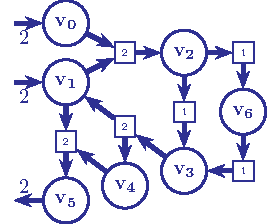
\includegraphics[scale=1.4]{graphics/chapter4/overlap.pdf}
        \vspace{0.5cm}
        \caption{An integer hyperflow satisfying all constraints listed in Section~\ref{implemented_model}. However, it is just the superposition of the solutions~\ref{fig:solution1} and~\ref{fig:solution2}.}
        \label{fig:overlap}
    \end{subfigure}
    \vspace{0.5cm}
    \caption{Addition of constrain~\eqref{subset_elimination} removes solutions like those shown in~\ref{fig:overlap} from the enumerated solutions.}
    \label{fig: union_solutions}
\end{figure}

However, in our case initial experimentation showed that using this enumeration policy, later enumerated solutions $f_2$ often contained a previous solution $f_1$, in the sense that $supp(f_1) \subsetneq supp(f_2)$, as exemplified in Figures~\ref{fig: cover} and~\ref{fig: union_solutions}.
To increase diversity of solutions, we opted for a custom enumeration scheme where $supp(f_2)$ of new solution~$f_2$ cannot contain $supp(f_1)$ of a previous solution~$f_1$ as a subset. When $supp(f_1) \subsetneq supp(f_2)$ holds for for a pair of solutions, the following statement must evaluate to \textsc{true} for the solution $f_1$:

\begin{center}
\begin{tabular}{lrl}
    & $\neg \bigwedge_{e\in supp(f_2)} z_e$ & $=$ TRUE\\
    or,& $\bigvee_{e\in supp(f_2)} \neg z_e$ & $=$ TRUE\\
    or,& $\sum_{e\in supp(f_2)} (1 - z_e)$ & $\geq 1$\\
    or,& $|supp(f_2)| - \sum_{e\in supp(f_2)} z_e$ & $\geq 1$\\
    or,& $\sum_{e\in supp(f_2)} z_e$ & $\leq |supp(f_2)| - 1$
\end{tabular}
\end{center}

In more detail: Let $f_i$ be the $i$th solution found. 
We then disallow subsequent solutions to contain $supp(f_i)$ by requiring that at least one of the hyperedges of~$f_i$ is not used. This is expressed via the following constraint:
\begin{equation}
    \sum_{e\in supp(f_i)} z_e \leq |supp(f_i)| - 1
    \label{subset_elimination}
\end{equation}
This constraint ensure that not all of the hyperedges in solution $f_i$ is used in some subsequent solution.
When the $k$th solution is to be found, there has thus been added $k-1$ of these constraints in total.
However, this method works only when the set of variables enumerated over is boolean, as is the case with $z_e$.

In Figure~\ref{fig: cover}, the hyperflow of the entire figure (with the part with lower opacity) has a subset of hyperedges which form a solution by itself. Therefore, $\bigwedge z_e$ evaluates to \texttt{TRUE} when evaluated over the set of hyperedges in the solution depicted in deep blue. Also, the left-hand side of the constraint~\ref{subset_elimination} is $\sum z_e = 4$ when evaluated over all the hyperedges in the hyperflow solution in dark blue which is $\nleq 4-1 = 3$. As a result, the hyperflow is not enumerated as a subsequent solution after the one in deep blue is added to the solution set.
Similarly the solution in Figure~\ref{fig:overlap}, would be excluded after either of the solutions in Figure~\ref{fig:solution1} or~\ref{fig:solution2} has been added to the solution set. The left-hand side of the constraint~\ref{subset_elimination} is $\sum z_e = 4$ when evaluated over all the hyperedges in the hyperflow in Figure~\ref{fig:solution1} which is $\nleq 4-1 = 3$. Therefore, the hyperflow in Figure~\ref{fig:overlap} is not enumerated as a subsequent solution after the one in Figure~\ref{fig:solution1} is added to the solution set. However, addition if the solution in Figure~\ref{fig:solution1} does not exclude the solution in~\ref{fig:solution2} as the left-side of constraint~\ref{subset_elimination} evaluates to $\sum z_e = 3$ (when summed over all hyperedges in the solution in Figure~\ref{fig:solution1}) which is $\leq 4-1 = 3$.

\subsection{Partial Ordering of Molecules}
\label{partial_order}

The ILP formulation of the problem~\cite{jakob_integer_hyperflows} accounts for the conservation of the for each molecule,
but not for temporal ordering of the reactions in the returned flow.
In scenarios such as synthesis planning~\cite{neurips_dag, rolf_synthesis_planning},
we would like to interpret a pathway as a directed acyclic process that generates the target molecule(s) unlike the one depicted in Figure~\ref{fig: selfLoop}.
We therefore introduce constraints to enforce a partial temporal order on the found pathways.

The ordering is implemented by introducing a supplementary integer variable $t_v$ for each vertex $v$ that keeps track of their ordering in the pathway.
The condition $t_{u} < t_{v}$ implies that the vertex $u$ is visited by the flow before the vertex $v$.
This is ensured by the following implication constraint:
\begin{align}
    \forall e\equiv (e^-, e^+)&\in E\colon \nonumber\\
        f_e &\geq 1 \implies t_v \geq t_u + 1, \label{prevent_back_edges}\\
        \forall &\text{ pairs } (u, v) \text{ such that } u \in e^-, v\in e^+ \nonumber
\end{align}

\begin{figure}[t]
    \centering
    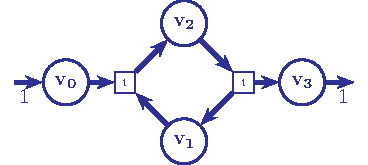
\includegraphics[scale=1.5]{graphics/chapter4/selfLoop.pdf}
    \caption{An example of a solution which satisfies the flow conservation constraint~\eqref{int_hyperflow_jakob} but cannot be realized if only $v_0$ is the allowed source and $v_3$ the requested target. To effect the first hyperedge, vertex $v_1$ is required to be present, which is in turn produced by the second hyperedge.
    Addition of constrain~\eqref{prevent_back_edges} remove such solution from being enumerated which are not physically realizable as a sequence of reaction to the target molecule(s).} 
    \label{fig: selfLoop}
\end{figure}

That is, the constraint ensures that reactants are assigned a lower order than products of a reaction with flow. 
We acknowledge that it can be too restrictive to enforce constraints to return pathways with an assigned partial ordering of vertices because they would eliminate all pathways with cycles in them.
Cycles are present whenever catalysts are used and in numerous metabolic networks.
We merely suggest the possibility of adding such constraints as part of the larger MILP model.
There might be other use cases where these partial constraints should be disabled in the model.
In these cases, the realizability question for pathways can be addressed using a separate,
more robust tool using the computationally more involved formalism of Petri nets on top of the MILP solver.
We refer the reader to a detailed study~\cite{sissel_realisability_petrinets} for a more thorough treatment of this issue of realizability of pathways.

\begin{figure}[!h]
    \centering
    \begin{subfigure}[b]{0.33\textwidth}
        \centering
        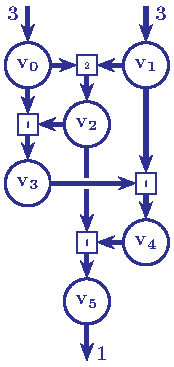
\includegraphics[scale=1.4]{graphics/chapter4/pathway_tvAssign.pdf}
    \end{subfigure}%
    \hspace{1cm}
    \begin{subfigure}[b]{0.5\textwidth}
        \centering
        \raisebox{3cm}{
		    \begin{tabular}{cc}
		    	\toprule
		    	vertex & $t_v$ \\
		   		\midrule
		    	$v_0$ & $0$ \\
		    	$v_1$ & $0$ \\
		    	$v_2$ & $1$ \\
		    	$v_3$ & $2$ \\
		    	$v_4$ & $3$ \\        
		    	$v_5$ & $5$ \\
		    	\bottomrule
			\end{tabular}
		}
    \end{subfigure}
    \caption{Addition of constrain~\eqref{linear_constraint8} ensures that the reactants are always available to effect a reaction either as products from a previous reaction or as sources. This prevents `back edges' in the pathway where are molecule is used that is produced later along the pathway.}
    \label{fig: partialOrderMolecules}
\end{figure}

The implication constraint in Equation~\eqref{prevent_back_edges} assigns the temporal ordering $t_v$ to each vertex $v$.
It is implemented as a linear constraint as
\begin{align}
    \forall \text{ pairs } (u, v)\,\,\,|\,\,\, \exists e\equiv (e^-, e^+) \text{ with } u &\in e^-, v \in e^+\colon \nonumber \\
    t_v - t_u - |V| (z_e - 1) - 1 &\geq 0 \label{linear_constraint8} \\
    \forall v\in V,\text{\hspace{1cm}}& \nonumber \\
    0 \leq t_v &\leq |V| \label{linear_constraint9}    
\end{align}
The constraint in Equation~\eqref{linear_constraint8} enforces the assignment $t_{v} > t_{u}$ only if the corresponding hyperedge is used in the hyperflow.
The size of the set of vertices in the hypergraph $|V|$ is used instead of the large integer $M$ in the constraint in Equation~\eqref{linear_constraint8} and as an upper bound for the temporal ordering variable $t_v$ for each vertex $v$ in the constraint in Equation~\eqref{linear_constraint9}.
The number of constraints added to the MILP model to determine the topological sorting of the vertices is $\mathcal{O}\left(|V|^2\right)$.

\section{Comparison with other methods}
\label{ch:discussions}

Previous work such as~\cite{shortest_path_hypergraph1,shortest_path_hypergraph2} have utilized hyperpaths in directed hypergraphs to depict pathways in reaction networks. However, they use the notion of path length to characterize the goodness of the pathway: a shorter pathway is considered better. Often this might not be the case as the shortest pathway might contain a slow or a high-cost reaction, which becomes a bottleneck for the entire pathway. Therefore, it is important to consider some physical attributes of the reactions (such as the barrier heights) in addition to the number of reactions while searching for pathways.

Most of previous work~\cite{graph_network1,graph_network2,graph_network3,heuristic_expert,reported_network} related to searching for pathways in reaction networks represent the underlying network as a graph with simple edges. However, this does not capture the nature of chemical reactions faithfully as it might involve multiple reactant molecules and produce multiple product molecules. Often the modeling tracks the most important molecules in the reactions~\cite{yaks,yarp}, relegating the other molecules involved in the reaction as reagents or side-products (in the style of synthesis maps of natural products). However, since the mathematical framework of hypergraphs exists to represent many-to-many mappings, we choose to use it instead of graphs. This has only one drawback: the visualization of the reaction networks becomes a little more involved and non-intuitive.

Studies focusing on large reaction networks such as~\cite{crn_expand_qm,shortest_path_hypergraph1,shortest_path_hypergraph2,reported_network} often extract the network from databases or existing knowledge. In contrast, using a generative methodology which can create the network on the fly (from a set of input molecules and a set of rules representing classes of reactions) allows us to investigate regions of the molecular space what have not been studied before. Moreover, it removes biases from previous experiments and studies that might have crept in while curating the database. If a particular promising molecule is not entered into the database, then no pathways queried from that network will contain it.

While there exists prior work which includes the generation of reaction networks, these networks were mostly generated using the gradient of potential information~\cite{iminoacetaldehyde2,yarp,empi1}. The determination of the gradient information used in potential energy surface explorations is computationally expensive and might limit the size of the studied network. Such studies focus on expanding the network only in the most promising directions and do not consider the remaining molecular space. Such a choice necessitated by computational costs hinders a thorough examination of the molecular space for pathways.  Chemical heuristics used by~\cite{yaks,heuristic_expert} offers a way out of this problem, and our method uses reaction templates to generate the networks this other studies in this class. We aim to generate an exhaustive network that is an over-approximation of what actually occurs in the system. The use of reaction templates allows us to cover all reaction possibilities in the generated network with a manageable computational cost. The current method uses graph rewriting and double pushouts as the formal framework behind the expansion of the network, which to the best of our knowledge is not used in other similar works.



\printbibliography[
  heading=subbibliography,
  title={References}
]

\end{refsection}

%************************************************
\chapter[Glycolonitrile Chemistry]{Case study: Glycolonitrile Chemistry}
\label{ch:casestudy2} %
%************************************************

\definecolor{mygray}{gray}{0.9}
\definecolor{myBlue}{rgb}{0.0, 0.2, 0.6}
\definecolor{myGreen}{rgb}{0.1, 0.5, 0.0}
\definecolor{myBrown}{rgb} {0.43, 0.21, 0.1}
\definecolor{myCyan}{rgb}{0.0, 0.58, 0.71}
\definecolor{myBlue2}{rgb}{0.36, 0.57, 0.9}
\definecolor{myRed}{rgb}{0.87, 0.36, 0.51}

{\sffamily\slshape The text in this chapter is identical to Section 4 of the published version of the preprint at \href{https://arxiv.org/abs/2504.10609}{arXiv:2504.10609}.\\}

In this chapter, we apply the methods from Chapter~\ref{ch:refined_model} to a reaction network generated in silico from glycolonitrile (or more formally 2-hydroxyethanenitrile), ammonia (NH$_3$), and water (H$_2$O), a network previously studied in \cite{implemented_CRN}. The choice of 2-hydroxyethanenitrile as the starting molecule was driven by the fact that it has been reported to occur in interstellar medium as a product of the condensation of methanal with hydrogen cyanide and act as a precursor to important molecules in pre-biotic systems~\cite{MeCN_precursor}. The previous work~\cite{implemented_CRN} constructed a free-energy map of the molecules that might be present when 2-hydroxyethanenitrile reacts with water and ammonia using computationally-intensive density functional theory calculations. It focused on finding thermodynamic sinks and kinetic barriers in the different regions of the free energy landscape.

\section{Network Generation}

In this chapter, the network was expanded using the graph transformation based generative framework M{\O}D \cite{mod_web}. The generation of the network, starting from the three above-mentioned molecules was done through the recursive application of the three graph transformation rules shown in Figure~\ref{fig:graphTransformationRules}.
A graph transformation rules (to repeat what was already stated in Chapter~\ref{ch:casestudy1}) is a template representing a class of reactions, which share the same set of atoms involved in the reaction, with similar changes in the bond set. The left hand side of the rules is a subgraph (representing a molecular fragment), which can be rewritten as the subgraph on the right hand side, when a match is found in one of the graphs representing molecules already present in the reaction network. This executes a reaction, adding the new product molecules and the reaction the reaction network, and expands the molecular space.

\begin{figure}[!t]
    \centering
    \begin{subfigure}{\textwidth}
        \centering
        \includegraphics[scale=1.5]{graphics/chapter5/rule0.pdf}
        \caption{Addition to a cyanide: in this rule \texttt{x} $\in$ \{N, O\}, representing the addition of an amide nitrogen or hydroxyl oxygen to the nitrile bond respectively.}
        \label{fig: rule0}
    \end{subfigure}
    \\
    \vspace{0.5cm}
    \begin{subfigure}{\textwidth}
        \centering
        \includegraphics[scale=1.5]{graphics/chapter5/rule1.pdf}
        \caption{Addition to an imine or carbonyl: in this rule \texttt{x}, \texttt{y} $\in$ \{N, O\}, representing the addition of an amide nitrogen or hydroxyl oxygen to an amide or hydroxyl bond respectively. This single rule encapsulates $2^2 = 4$ individual rules depending on the instantiation of \texttt{x} and \texttt{y}.}
        \label{fig: rule1}
    \end{subfigure}
    \\
    \vspace{0.5cm}
    \begin{subfigure}{\textwidth}
        \centering
        \includegraphics[scale=1.5]{graphics/chapter5/rule2.pdf}
        \caption{1,3 hydrogen shift: in this rule \texttt{x}, \texttt{y} $\in$ \{C, N, O\}, representing the shift of a double bond as in tautomerism. When \texttt{x}$\equiv$O and \texttt{y}$\equiv$O it is keto-enol tautomerism, \texttt{x}$\equiv$N and \texttt{y}$\equiv$N is imine-enamine tautomerism, \texttt{x}$\equiv$N and \texttt{y}$\equiv$O is amine-iminol tautomerism and \texttt{x}$\equiv$C and \texttt{y}$\equiv$C is an allylic shift of the double bond. This single rule encapsulates $3\times 3 = 9$ individual rules depending on the instantiation of \texttt{x} and \texttt{y}.}
        \label{fig: rule2}
    \end{subfigure}
    \vspace{0.2cm}
    \caption{The graph transformation rules used to expand the molecular space and generate the network. The inverse of all the three graph transofrmation rules were also used while generating the reaction network.}
    \label{fig:graphTransformationRules}
\end{figure}

\begin{figure}[!t]
	\centering
	\vspace{0.5cm}
    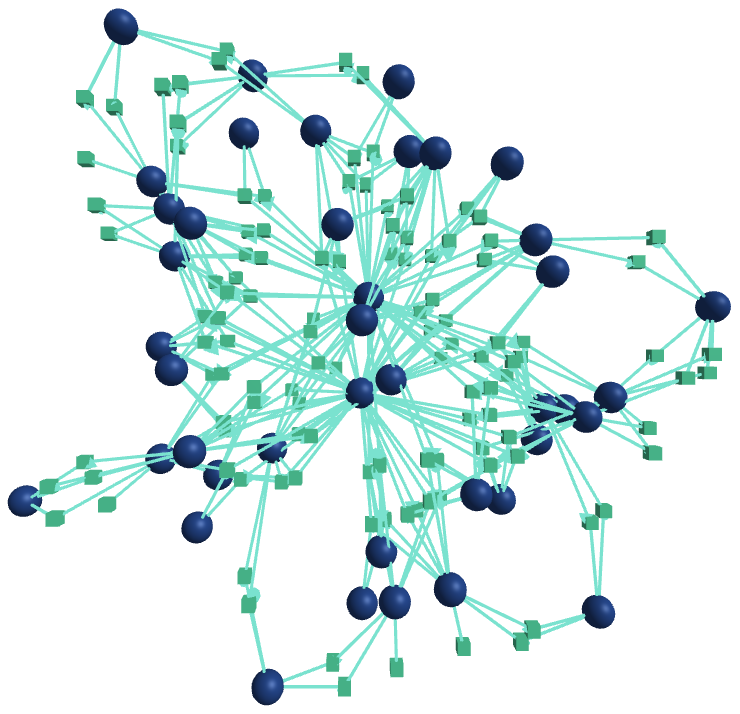
\includegraphics[width=0.8\textwidth]{graphics/chapter5/reactionNetworkChapter5.png}
    \vspace{0.5cm}
    \caption{An abstract representation of the generated reaction network with $44$ vertices (blue circles) and $116$ hyperedges (green squares), on which the working of the method proposed in Chapter~\ref{ch:refined_model} was demonstrated.}
    \label{fig: hypergraphRNChapter5}
\end{figure}

Molecules with up to two carbon, four nitrogen, and four oxygen atoms were included in the generated network for comparability with \cite{implemented_CRN}, which considered molecules with two carbon atoms only. The constructed reaction network had $44$ vertices and $116$ hyperedges, and shown in Figure~\ref{fig: hypergraphRNChapter5}. 
A list of molecules and reactions in the generated network is available in the GitHub data repository.  
To find probable pathways to biologically important molecules of glycine and glycolic acid, the structures of which are shown in Figure~\ref{fig:target0} and~\ref{fig:target1} respectively, using glycolonitrile, NH$_3$, and H$_2$O, an ILP was formulated to query the desired pathways.
The formulated ILP had $336$ variables and $1561$ constraints.
The reason for choosing glycine is that it is the simplest amino acid and can be considered as the building block of proteins which are essential for life. Glycolic acid is also widespread in nature in the form of glycolate salts which are produced during photorespiration in plants.
 
\begin{figure}[!t]
    \centering
    \begin{subfigure}{0.45\textwidth}
        \centering
        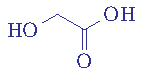
\includegraphics[scale=1.0]{graphics/chapter5/glycine.pdf}
        \caption{glycine}
        \label{fig:target0}
    \end{subfigure}
    \hfill
    \begin{subfigure}{0.45\textwidth}
        \centering
        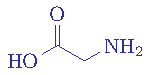
\includegraphics[scale=1.0]{graphics/chapter5/glycolic acid.pdf}
        \caption{glycolic acid}
        \label{fig:target1}
    \end{subfigure}
    \caption{target molecules in the flow query.}
    \label{fig:targetMolecules}
\end{figure}

\section{Pathways to Glycine}

The five best scoring pathways to the target glycine is depicted in Figure \ref{fig:pathway1}.
The structures for the molecules in the corresponding vertices is listed in Table \ref{tab:molecular_structures1} and the weights assigned to the hyperedges listed in Table \ref{tab:pathways1}.
The \textcolor{myBlue}{best scoring pathway} scores $143118$ on the chosen objective \eqref{proposed_objective} and proceeds through 2-iminoethanal ($v_6$), a pre-biotic intermediate hypothesized to be of significance. 
A water molecule acts as a catalyst in this pathway since it is used in reaction $e_1$ and generated back in reaction $e_4$. 
The \textcolor{myGreen}{second best pathway} scores $143190$ on the objective \eqref{proposed_objective}. The last two reactions are the same for both (in fact, for all \emph{five}) pathways. 
This second best pathway uses an ammonia molecule as a catalyst, molecules with a higher chemical potential (under unit concentrations) and reactions with higher energy barriers. The sum of the energy barriers for the reactions in this pathway is $200.02$ kJ mol$^{-1}$ as opposed to $128.74$ kJ mol$^{-1}$ for the best pathway. 
One might note that the difference in the objective value of the best and the second-best solutions, that is $143190-143118 = 72$ is entirely due to the difference in the sum of the energy barriers of the reactions along the pathway ($(200 - 128)$ kJ mol$^{-1} = 72$ kJ mol$^{-1}$) or the first part of the ovjective \eqref{proposed_objective} because both the pathways have the same length. Both pathways consist of $6$ reactions and the second part of the objective \eqref{proposed_objective} is the same for both solutions.

The \textcolor{myBrown}{third pathway} branches off the second pathway and merges into the first, with a different reaction $e_4$ eliminating an ammonia molecule. This ammonia molecules was added to glycolonitrile in the first step and therefore, acts as a catalyst in the pathway.
The \textcolor{myCyan}{fourth pathway} uses a different molecule instead of iminoacetaldehyde, which has a higher chemical potential, hence is ranked lower than the previous three. 
The \textcolor{myBlue2}{fifth pathway} has \emph{eight} reactions, while the previous four had seven reactions. Despite having a lower sum of the energy barriers ($152.90$ kJ mol$^{-1}$), it is ranked lower than the previous three pathways because it is longer.
This exemplifies how the length of the pathways affects its ranking through the second part of the objective \eqref{proposed_objective}.
Figure \ref{fig:pathway1} shows how interconnected the individual different pathways in the network might be, often with parallel branches and cross-connections, which leads to complex behavior of the system. 

The estimated energy barriers for the reactions used in the reported pathways in Figure \ref{fig:pathway1} is presented in Table \ref{tab:pathways1}. Table \ref{tab:pathways1} consists of five columns that list the assigned weights for the hyperedges in the pathways shown in Figure \ref{fig:pathway1}. 
The shaded cells indicate hyperedges that have already been used in a previously enumerated pathway. For instance, all five pathways in Figure \ref{fig:pathway1} share the final two reactions. Consequently, the next four pathways reuse the last two reactions of the first pathway, and the last two rows for the corresponding columns are shaded to reflect this overlap.  

Ab initio molecular dynamics has been used in a previous work~\cite{crn_expand_qm3,glycine_pathway} to simulate the Urey-Miller experiment and find possible pathways to glycine in a prebiotic setting. The reported pathways in~\cite{crn_expand_qm3} also contain reactions catalysed by water and ammonia. The reported pathways to glycine in~\cite{crn_expand_qm3} proceeds through a singlet carbene intermediate, while those in~\cite{glycine_pathway} has a molecule with a three-membered ring, oxiranimine, as an intermediate. However, in the current work, there were no reaction templates used which might lead to the formation of a carbene-like molecule or a three-cycle in a molecule in the generated network. Hence, such a pathway was not observed. Carbenes and three-cycles are highly reactive intermediates, and their formation is a high energy process. On the whole, the pathways presented in this work have much lower reported energy barriers than that reported in these two studies.


\begin{figure}[!thb]
    \centering
    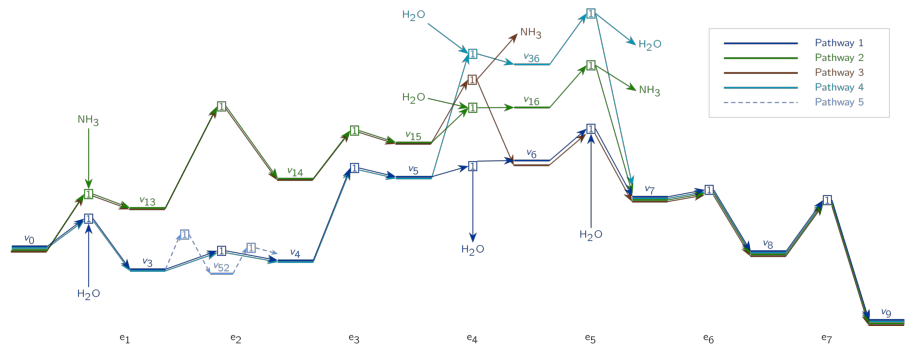
\includegraphics[width=\linewidth]{graphics/chapter5/pathway1.pdf}
    \vspace{0.4cm}\\
    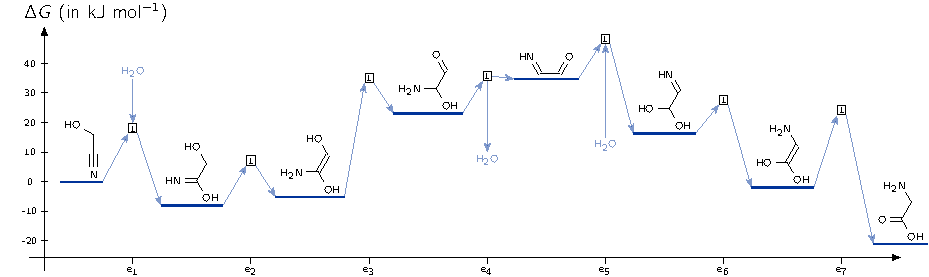
\includegraphics[width=\linewidth]{graphics/chapter5/bestPathway1.pdf}
    \vspace{0.1cm}
    \caption{Top: A schematic depiction of the five best pathways to glycine according to the chosen scoring function (energy levels not shown exactly to scale).   
    Bottom: The energy profile of the best-scoring pathway (in blue) from above (energy levels shown to scale) wth the molecular structures explicitly shown.}
    \label{fig:pathway1}
\end{figure}

\begin{figure}[!thb]
	\vspace{0.5cm}
	\begin{subfigure}{0.65\textwidth}
    	\centering
    	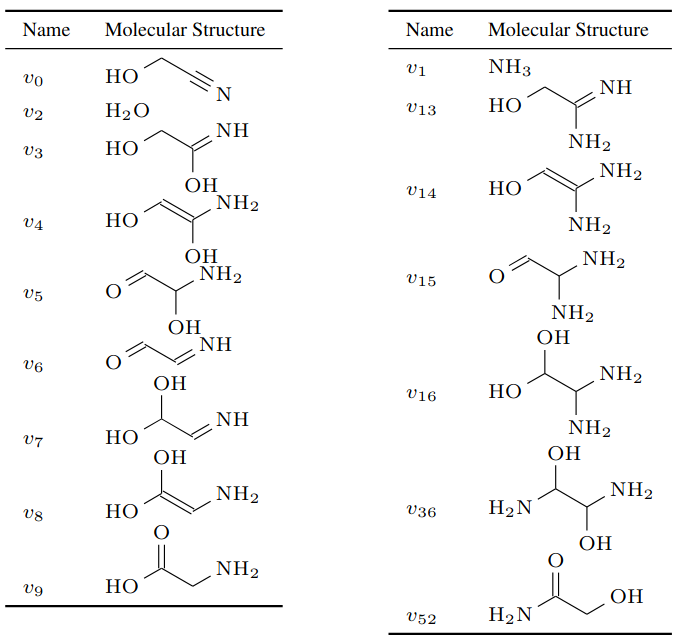
\includegraphics[scale=0.3]{graphics/chapter5/molStrucPathway1.png}
    	\caption{Molecular graphs in the pathways in Figure \ref{fig:pathway1}.}
    	\label{tab:molecular_structures1}
    \end{subfigure}%
    \begin{subfigure}{0.3\textwidth}
    	\centering
    	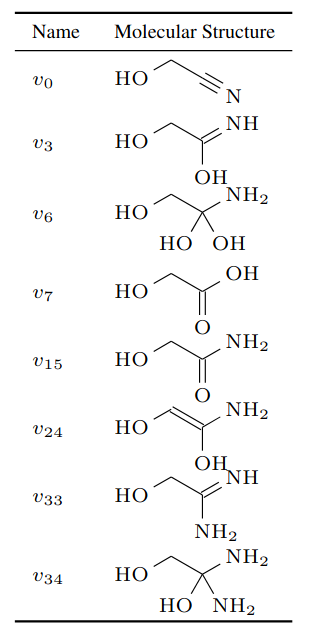
\includegraphics[scale=0.3]{graphics/chapter5/molStrucPathway2.png}
    	\caption{and in Figure \ref{fig:pathway2}}
    	\label{tab:molecular_structures2}
    \end{subfigure}
    \caption{List of the molecular structures corresponding to the the labeled vertices in the pathways in Figures~\ref{fig:pathway1} and~\ref{fig:pathway2}.}
\end{figure}

\begin{table}[!h]
    \centering
    \vspace{1cm}
    \begin{footnotesize}
    \begin{adjustbox}{angle=90}
    \begin{tabular}{lrrrrr}
        \toprule
        Reaction\hspace{0.2cm} & \multicolumn{5}{c}{Energy barriers (in kJ mol$^{-1}$)} \\
        count & \hspace{1cm}\textcolor{myBlue}{pathway 1} & \hspace{1cm}\textcolor{myGreen}{pathway 2} & \hspace{1cm}\textcolor{myBrown}{pathway 3} & \hspace{1cm}\textcolor{myCyan}{pathway 4} & \hspace{1cm}\textcolor{myBlue2}{pathway 5} \\
        \midrule
        \multirow{2}{*}{$e_1$} & $13.95$ & $33.18$ & \cellcolor{mygray}$33.18$ & \cellcolor{mygray}$13.95$ & \cellcolor{mygray}$13.95$\\
        & $(v_0+v_2, v_3)$ & $(v_0+v_1, v_{13})$ & \cellcolor{mygray}$(v_0+v_1, v_{13})$ & \cellcolor{mygray}$(v_0+v_2, v_3)$ & \cellcolor{mygray}$(v_0+v_2, v_3)$  \\
        \multirow{2}{*}{$e_2$} & $7.67$ & $64.17$ & \cellcolor{mygray}$64.17$ & \cellcolor{mygray}$7.67$ & $18.67, 13.15$\\
        & $(v_3, v_4)$ & $(v_{13}, v_{14})$ & \cellcolor{mygray}$(v_{13}, v_{14})$ & \cellcolor{mygray}$(v_3, v_4)$ & $(v_3, v_{52}, v_4)$ \\
        \multirow{2}{*}{$e_3$} & $57.69$ & $28.40$ & \cellcolor{mygray}$28.40$ & \cellcolor{mygray}$57.69$ & \cellcolor{mygray}$57.69$\\
        & $(v_4, v_5)$ & $(v_{14}, v_{15})$ & \cellcolor{mygray}$(v_{14}, v_{15})$ & \cellcolor{mygray}$(v_4, v_5)$ & \cellcolor{mygray}$(v_4, v_5)$\\
        \multirow{2}{*}{$e_4$} & $1.67$ & $19.86$ & $29.35$ & $67.36$ & \cellcolor{mygray}$1.67$\\
        & $(v_5, v_6+v_2)$ & $(v_{15}+v_2, v_{16})$ & $(v_{15}, v_6+v_1)$ & $(v_5+v_2, v_{36})$ & \cellcolor{mygray}$(v_5, v_6+v_2)$\\
        \multirow{2}{*}{$e_5$} & $17.14$ & $23.79$ & \cellcolor{mygray}$17.14$ & $60.84$ & \cellcolor{mygray}$17.14$ \\\
        & $(v_6+v_2, v_7)$ & $(v_{16}, v_7+v_1)$ & \cellcolor{mygray}$(v_6+v_2, v_7)$& $(v_{36}, v_7+v_2)$ & \cellcolor{mygray}$(v_6+v_2, v_7)$\\
        \multirow{2}{*}{$e_6$} & $0.19$ & \cellcolor{mygray}$0.19$ & \cellcolor{mygray}$0.19$ & \cellcolor{mygray}$0.19$ & \cellcolor{mygray}$0.19$ \\
        & $(v_7, v_8)$ & \cellcolor{mygray}$(v_7, v_8)$ & \cellcolor{mygray}$(v_7, v_8)$ & \cellcolor{mygray}$(v_7, v_8)$ & \cellcolor{mygray}$(v_7, v_8)$\\
        \multirow{2}{*}{$e_7$} & $30.42$ & \cellcolor{mygray}$30.42$ & \cellcolor{mygray}$30.42$ & \cellcolor{mygray}$30.42$ & \cellcolor{mygray}$30.42$ \\
        & $(v_8, v_9)$ & \cellcolor{mygray}$(v_8, v_9)$ & \cellcolor{mygray}$(v_8, v_9)$ & \cellcolor{mygray}$(v_8, v_9)$ & \cellcolor{mygray}$(v_8, v_9)$\\
        \midrule
        sum & $128.74$ & $200.02$ & $202.85$ & $238.13$ & $152.90$ \\
        \bottomrule
    \end{tabular}
    \end{adjustbox}
    \end{footnotesize}
    \vspace{1cm}
    \caption{From the left, the columns list the weights assigned to the hyperedges along with the sum of the weights, for the five pathways in Figure \ref{fig:pathway1}.}
    \label{tab:pathways1}
\end{table}

\begin{table}[!h]
    \centering
    \vspace{0.5cm}
    \begin{footnotesize}
    \begin{adjustbox}{angle=90}
    \begin{tabular}{lrrrrrr}
        \toprule
        Reaction\hspace{0.2cm} & \multicolumn{6}{c}{Energy barrier} \\
        count & \hspace{0.5cm}\textcolor{myBlue}{pathway 1} & \hspace{0.5cm}\textcolor{myGreen}{pathway 2} & \hspace{0.5cm}\textcolor{myBrown}{pathway 3} & \hspace{0.5cm}\textcolor{myCyan}{pathway 4} & \hspace{0.5cm}\textcolor{myBlue2}{pathway 5} & \hspace{0.5cm}\textcolor{myRed}{pathway 6} \\
        \midrule
        \multirow{2}{*}{$e_1$} & $13.95$ & \cellcolor{mygray}$13.95$ & \cellcolor{mygray}$13.95$ & \cellcolor{mygray}$33.18$ & \cellcolor{mygray}$13.95$ & \cellcolor{mygray}$33.18$\\
        & $(v_0+v_2,v_3)$ & \cellcolor{mygray}$(v_0+v_2,v_3)$ & \cellcolor{mygray}$(v_0+v_2,v_3)$ & \cellcolor{mygray}$(v_0+v_1,v_{33})$ & \cellcolor{mygray}$(v_0+v_2,v_3)$ & \cellcolor{mygray}$(v_0+v_1,v_{3}3)$\\
        \multirow{2}{*}{$e_2$} & & & $7.67$ & $48.612$ & $80.53$ & \cellcolor{mygray}$48.61$\\
        & & & $(v_3, v_{24})$ & $(v_{33}+v_2, v_{34})$ & $(v_3+v_1, v_{34})$ & \cellcolor{mygray}$(v_{33}+v_2, v_{34})$\\
        \multirow{2}{*}{$e_3$} & $26.61$ & $18.68$ & $11.76$ & $43.64$ & \cellcolor{mygray}$43.64$ & $33.08$\\
        & $(v_3+v_2, v_6)$ & $(v_3, v_{15})$ & $(v_{24}, v_{15})$ & $(v_{34}, v_{15}+v_1)$ & \cellcolor{mygray}$(v_{34}, v_{15}+v_1)$ & $(v_{34}, v_3+v_1)$\\
        \multirow{2}{*}{$e_4$} & & $0.62$ & \cellcolor{mygray}$0.62$ & \cellcolor{mygray}$0.62$ & \cellcolor{mygray}$0.62$ & \cellcolor{mygray}$0.62$\\
        & & $(v_{15}+v_2,v_6)$ & \cellcolor{mygray}$(v_{15}+v_2,v_6)$ & \cellcolor{mygray}$(v_{15}+v_2,v_6)$ & \cellcolor{mygray}$(v_{15}+v_2,v_6)$ & \cellcolor{mygray}$(v_3+v_2,v_6)$\\
        \multirow{2}{*}{$e_5$} & $74.62$ & \cellcolor{mygray}$74.62$ & \cellcolor{mygray}$74.62$ & \cellcolor{mygray}$74.62$ & \cellcolor{mygray}$74.62$ & \cellcolor{mygray}$74.62$ \\
        & $(v_6, v_7+v_1)$ & \cellcolor{mygray}$(v_6, v_7+v_1)$ & \cellcolor{mygray}$(v_6, v_7+v_1)$ & \cellcolor{mygray}$(v_6, v_7+v_1)$ & \cellcolor{mygray}$(v_6, v_7+v_1)$ & \cellcolor{mygray}$(v_6, v_7+v_1)$\\
        \midrule
        sum & $118.19$ & $107.87$ & $108.63$ & $200.68$ & $213.38$ & $219.11$  \\
        \bottomrule
    \end{tabular}
    \end{adjustbox}
    \end{footnotesize}
    \vspace{0.5cm}
    \caption{From the left, the columns list the weights assigned to the hyperedges along with the sum of the weights, for the six pathways in Figure \ref{fig:pathway2}.}
    \label{tab:pathways2}
\end{table}

\section{Pathways to Glyoxlic acid}

\begin{figure}[!t]
    \centering
    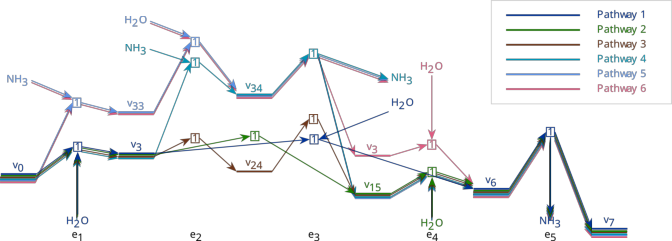
\includegraphics[width=\linewidth]{graphics/chapter5/pathway2.pdf}
    \caption{The six best pathways to glyoxlic acid according to the chosen scoring function.
    The best scoring pathway is depicted in blue, and the next best pathways in green, brown, cyan, azure and red. 
    The structures for the molecules for the vertices is listed in Table \ref{tab:molecular_structures2} and the weights assigned to the hyperedges listed in Table \ref{tab:pathways2}.}
    \label{fig:pathway2}
\end{figure}

\begin{figure}[!thb]
	\vspace{0.5cm}
    
\end{figure}

Another molecule of importance in prebiotic systems which appears in the generated network is 2-hydroxyethanoic acid, commonly known ad glycolic acid. During photorespiration plants produce glycolate. It can also be used as a monomer for various biodegradable polymers such as polyglycolic acid and poly(lactic-co-glycolic) acid. However, there have not been many studies on pathways to glyocolic acid from the precursor molecules in prebiotic systems.  
Figure \ref{fig:pathway2} shows the six best pathways to 2-hydroxyethanoic acid along with the molecules used in the pathway in Table~\ref{tab:molecular_structures2}. The \textcolor{myBlue}{best scoring pathway} has three reactions, the \textcolor{myGreen}{second best} has four reaction, while the rest involve five reactions. Despite the third-listed pathway having a lower sum of energy barriers ($108.63$ kJ mol$^{-1}$), it is ranked lower because it is longer, illustrating the effect of the second term in the objective \eqref{proposed_objective}. 

Table \ref{tab:pathways2} contains six columns that list the assigned weights for the hyperedges in the pathways illustrated in Figure \ref{fig:pathway2}. As in Table \ref{tab:pathways1}, the shaded cells indicate hyperedges that have already been used in a previously enumerated pathway. The specific hyperedge is mentioned below the energy barrier, with the reactants as the first element of the pair and the products as the second element. Individual molecules are separated by a `+', and the structures of the molecules the labels correspond to can be looked up from Table \ref{tab:molecular_structures2}. 

The expansion of the network shown in Figure~\ref{fig: hypergraphRNChapter5} took 67 seconds. It is quite faster than comparable methods using reaction templates without using graph transformation, molecular dynamics or potential energy search as done in~\cite{implemented_CRN}. Annotating the $116$ hyperedges with the energy barriers of the reactions as weights took around an hour. Using a neural network instead of more accurate traditional methods does lead to trade off of the accuracy for speed, but it allows scalability for larger networks. Formulating the ILP and enumerating the pathways in the network to the two target molecules using the objective function \eqref{proposed_objective} took around $52$ seconds. All the reported times are the average of $10$ runs on an AMD$^{\circledR}$ Ryzen 5 PRO 4650U CPU (2.1 GHz) utilizing $8$ threads.


%************************************************
\chapter{Summary}
\label{ch:conclusion} %
%************************************************

{\sffamily\slshape The text in this chapter is based on Section 6 of the published versions of the preprints at \href{https://arxiv.org/abs/2411.15900}{arXiv:2411.15900} and \href{https://arxiv.org/abs/2504.10609}{arXiv:2504.10609} and  Section 5 of the preprint at \href{https://arxiv.org/abs/2504.10609}{arXiv.2607.04160}.\\}

Thermodynamics emerged from efforts to analyze the operation of steam engines while maximizing their work.
In a nice analogy, the search for pathways may be phrased as viewing reaction networks as chemical engines in which we want to maximize the output of some target molecule(s).
Recognizing that thermodynamics, encapsulated by the Gibbs free energies of the reactions, play a pivotal role in determining the probability of a reaction, Chapter~\ref{ch:thermodynamic_model} focused on developing ways to integrate them into the search for pathways.

Exploring pathways with favorable energy profiles involves challenging navigation of a large and complex energy landscape where the driving thermodynamic forces are influenced by the concentration ratios, inflows of the source molecules, and outflows of the target molecules.
Chapter~\ref{ch:thermodynamic_model} attempted to address part of that challenge.
However, there might be several refinements possible to the model proposed in Chapter~\ref{ch:thermodynamic_model}, some of which we list here:
\begin{enumerate}
    \item The constraint enforcing that only reactions with negative free energies are allowed in the returned pathways (implemented through the constraint in Equation~\eqref{proposed_constraint3}) may be overly stringent.
    Under experimental conditions, the reactions observed to occur do not always align with those predicted to occur theoretically: the thermal decomposition of lithium carbonate is observed to occur in practice despite being predicted to be thermodynamically unfavorable using computed (or experimental) free energies for the reaction.
    However, reactions predicted to be thermodynamically favorable do not always occur in practice because they have a high energy barrier (like the allotropic conversion of diamond into graphite).
    Therefore, there should be some flexibility in delineating the boundary between those reactions that are considered likely and included in the pathway and those that are not, to bring the model closer to reality. 
    Such extensions of the current modeling should be fairly straightforward.
    \item The objective function minimizes the sum of the Gibbs free energies of the reactions in the pathway.
    However, this approach might favor a pathway with more extreme values for the free energies rather than one with more moderate free energy values.
    Therefore, it might be worthwhile to explore alternative objective functions, such as the min-max, in addition to the min-sum used here.
    \item The current formulation disregards the kinetics of individual reactions.
    However, the probability of a reaction occurring is determined to a substantial extent by the reaction barrier height, and not only by the concentration of the reactants and the products.
    As a result, our framework might include a reaction in the returned pathway with a favorable thermodynamic driving force but too high a reaction barrier, making it a slow and rate-limiting step for the entire pathway.
    On the other hand, coming up with a generic `kinetic oracle' with wide applicability to estimate the barrier heights for diverse reactions poses a significant challenge.
    The transition states determining the barrier heights are saddle points on the potential energy surface, unlike reactants or products that are minima and can be located by gradient descent optimization methods. 
\end{enumerate}

Hence, we do not claim that the model proposed in Chapter~\ref{ch:thermodynamic_model} to be the final in the quest to incorporate thermodynamics into the search for pathways in reaction networks.
Still, we believe that it constitutes a valuable step forward, and we end by summarizing its virtues.
We provide a systematic and thermodynamically informed approach to optimize the computational search for pathways in reaction networks.

Modeling pathways as integer hyperflows gives results that can be interpreted in mechanistic terms,
as each molecule is present in integral quantities.
Formulating the problem as an MILP problem and utilizing an MILP solver allows us to obtain solutions with reasonable computational resources and time.
It allows enumeration of pathways over the integral flow variables, facilitating a systematic exploration of pathways in the reaction network.
Returning several solutions to pathway queries is an asset, as the answer becomes more robust to possible errors in the calculations of chemical potentials of the molecules and to other artifacts of the simplification of reality inherent in any modeling.
Moreover, it offers alternatives to choose from if the optimal solution turns out to be unattainable under controlled industrial reactor or laboratory conditions. 

Finally, the application of the framework formulated in Chapter~\ref{ch:thermodynamic_model} to a reaction network, in Chapter~\ref{ch:casestudy1}, based on real-life chemistry acts as a proof-of-concept and illustrates the computational feasibility and analytic potential of our methods.

In Chapter~\ref{ch:refined_model}, we have described a methodology for kinetically informed exploration of pathways in reaction networks building on the model proposed in Chapter~\ref{ch:thermodynamic_model}. 
One part of the methodology is an automated workflow for annotating individual reactions with their energy barriers, computed using a diverse selection of tools---RDKit~\cite{rdkit_embedMolecule}, xTB~\cite{grimme_xtb}, ASE~\cite{ase-paper} and NeuralNEB~\cite{neuralneb}. The goal of this workflow is to minimize the laborious manual interventions and intensive expert knowledge often necessary when executing quantum chemical calculations to determine energy barriers. 
As demonstrated in Chapter~\ref{ch:casestudy2}, the workflow can be applied on networks of rather large scale, can work on the fly with generative network construction, and uses relatively moderate computational resources.
The method does not take into account the interactions of solvent molecules while calculating the energy barriers. This and the question of how well models based on machine learning generalize past their training sets may lead to reasonable reservations on the precision of the estimates of the energy barriers for some use cases. However, the proposed methodology offers the flexibility that this component can be substituted with alternatives, if desired.

As the other part of the proposed methodology, we formulated an ILP to query pathways in the annotated network and designed an objective function
for pathway evaluation. The query formalism is at the same time both precise and very flexible in what queries can be formulated. The objective function is made under the simplifying assumption that all molecules in the reaction network are present with unit concentrations at all times. Additionally, the costs assigned to pathways depend on the underlying reaction network considered, so comparisons across networks are not directly possible. However, the question of how to evaluate pathways is complex and the reader of course has the option to substitute a different objective function, based on other cost metrics. We do note, though, that our simplification and the formulation via ILP allows us to analyze much larger networks and using much less computational resources than alternatives like stochastic simulations or potential energy surface exploration.
We also note that by a progressive constraining of the ILP, we in the end can return a \emph{list} of high-scoring solutions, each representing structurally different pathways. Giving a list of good, structurally different solutions, rather than a single solution, helps mitigate disagreements about the details of pathway cost metrics.

Finally, the efficiency and utility of the method described in Chapter~\ref{ch:refined_model} was shown on a concrete reaction network in Chapter~\ref{ch:casestudy2}, studying pathways to pre-biotically significant molecules, such as glycine and 2-hydroxyethanoic acid. 

We have presented a framework for exploring reaction networks in Chapter~\ref{ch:stoc_explore}, motivated by chemical stochastic kinetics generating random walks on networks~\cite{randomwalk1,randomwalk2,randomwalk3} that differ from previous approaches. We do not precompute the network but rather discover regions of it through a process mimicking chemical stochastic dynamics. Instead of computing the relative probabilities for all possible reactions at each step, our method performs three modular sampling operations: (1) selecting a colliding molecular pair based on current molecular abundances, (2) selecting a reaction template, and (3) selecting a specific reaction instance generated by a graph transformation engine acting on that pair. In the example study presented in Chapter~\ref{ch:stoc_explore}, the reaction template probabilities are not intended to approximate physical rate laws, but rather to provide an unbiased sampling of dynamically reachable regions of a reaction graph defined on an atomistic level. This divide-and-conquer strategy avoids enumerating the full list of transitions out of the current state at every step and allows the dynamics to generate previously unvisited regions of chemical space on demand. In this sense, the method performs a biased random walk on an implicitly defined molecular network, constructing only the locally relevant subnetworks during the course of the exploration. 

Some key features of the framework proposed in the current work include the simultaneous use of (1) stochastic simulation-styled dynamics operating on molecular graphs (2) applying rule-based bond rearrangements on an atomic level using reaction templates to generate a relevant part of the molecular network on the fly and (3) the support of open systems with inflow and outflow on the system. 
It borrows from and straddles the region between the Gillespie algorithm for stochastic simulations (which is kinetically accurate but abstract), 
generative chemistry using graph grammar (which is chemically accurate but deterministic) and kinetic Monte Carlo simulations (which are stochastic but non-generative and closed). 
The simulation can be steered to explore the region of the molecular space under interest--- its parameters might also be biased to explore events which rarely occur under realistic conditions but are nevertheless important.
The present method provides a lightweight, highly scalable way to navigate regions of chemical space where kinetic parameters are unknown or where the objective is discovery rather than quantitative prediction.
It enables stochastic, network-free exploration of large, generative molecular spaces under minimal kinetic assumptions.
Together, with stochastic simulation schemes like the Gillespie algorithm or kinetic Monte Carlo, it forms two complementary probes to molecular networks: one for exact stochastic dynamics, one for graph-based exploration.

In summary, this work contributes to field of stochastical exploring large reaction networks and computationally assisted analysis and design of pathways in reaction networks represented as directed hypergraphs.



\backmatter
\printbibliography[
  %heading=subbibliography,
  title={References}
]

\input{backmatter/acknowledgements}

\end{document}

